% ============================================================
%  Anexo II - Análisis y Diseño del Sistema
%  Sistema de Gestión Documental mediante Blockchain
%  Compilar con: lualatex AnexoII_AnalisisDiseno.tex
% ============================================================

% ============================================================
% NOTA ENCODING (2026-03-27): Archivo corregido a UTF-8.
% Los caracteres acentuados (tildes) habian sido danados por
% una operacion de I/O con codificacion ISO-8859-1 en PS5.
% Patron 1 (AnexoI): U+FFFD para a/e/i/n/u; '?' para 'o'.
%   Solucion: diccionario de contexto + regex (fix_accents_v2.py, fix3.py).
% Patron 2 (AnexoII-V): todos los acentos como '?' literal.
%   Solucion: vacabulario de 462 entradas (fix_annexes_all.py, fix_final.py).
% REGLA: Siempre usar Python 3 + io.open(path,'w',encoding='utf-8').
%        NUNCA usar Set-Content de PowerShell 5 (anade BOM o rompe tildes).
% ============================================================
\documentclass[11pt, a4paper]{article}

\usepackage{fontspec}
\usepackage[spanish]{babel}
\usepackage{graphicx}
\usepackage{float}
\usepackage{amsmath}
\usepackage{xcolor}
\usepackage[protrusion=true,expansion=false]{microtype}
\usepackage{longtable}
\usepackage{array}
\usepackage{booktabs}
\usepackage{multirow}
\usepackage{caption}
\usepackage{pdflscape}
\usepackage{eso-pic}
\usepackage{tikz}
\usetikzlibrary{calc}
\usepackage[
    colorlinks = true,
    linkcolor  = black,
    urlcolor   = black,
    citecolor  = black
]{hyperref}

\usepackage{geometry}
\geometry{
    left       = 2.5cm,
    right      = 2.5cm,
    top        = 3cm,
    bottom     = 2.5cm,
    headheight = 55pt,
    headsep    = 0.8cm
}

\usepackage{listings}
\definecolor{lightgray}{rgb}{0.96, 0.96, 0.96}
\definecolor{darkblue}{rgb}{0.0, 0.0, 0.6}
\definecolor{darkorange}{rgb}{0.8, 0.4, 0.0}

\lstdefinelanguage{TypeScript}{
    keywords={break,case,catch,class,const,continue,debugger,default,delete,do,
              else,enum,export,extends,false,finally,for,function,if,import,in,
              instanceof,let,new,null,return,super,switch,this,throw,true,try,
              typeof,var,void,while,with,yield,async,await,interface,type,
              implements,private,protected,public,static,abstract,readonly},
    sensitive=true,
    comment=[l]{//},
    morecomment=[s]{/*}{*/},
    morestring=[b]',
    morestring=[b]",
    morestring=[b]`,
}

\lstdefinelanguage{Solidity}{
    keywords={pragma,solidity,contract,library,interface,function,modifier,event,
              struct,enum,mapping,address,bool,string,int,uint,bytes,public,
              private,internal,external,pure,view,payable,returns,memory,storage,
              calldata,emit,require,revert,assert,new,delete,this,super,
              constructor,fallback,receive,import,using,for,is},
    sensitive=true,
    comment=[l]{//},
    morecomment=[s]{/*}{*/},
    morestring=[b]',
    morestring=[b]",
}

\lstset{
    basicstyle      = \ttfamily\scriptsize,
    breaklines      = true,
    frame           = single,
    backgroundcolor = \color{lightgray},
    keywordstyle    = \color{darkblue}\bfseries,
    stringstyle     = \color{darkorange},
    showstringspaces= false,
}

\usepackage{fancyhdr}
\pagestyle{fancy}
\fancyhf{}

\lhead{
\includegraphics[height=1.25cm]{USAL-Logo-3820702873.png}}
\rhead{\shortstack[r]{\fontsize{10}{12}\selectfont\textbf{\tituloInforme}\\[-1pt]\fontsize{10}{12}\selectfont\subtituloInforme}}

\renewcommand{\headrulewidth}{0pt}
\renewcommand{\footrulewidth}{0pt}

\cfoot{%
        \color{gray}\rule[0.5ex]{0.4\textwidth}{0.8pt}%
        \hspace{0.5cm}%
        \textcolor{black}{\textbf{\thepage}}%
        \hspace{0.5cm}%
        \color{gray}\rule[0.5ex]{0.4\textwidth}{0.8pt}%
}

% ============================================================
% SOPORTE ENCABEZADO/PIE EN PÁGINAS APAISADAS (landscape)
% ============================================================
\newif\iflscape\lscapefalse

\let\origlandscape\landscape
\let\origendlandscape\endlandscape
\renewenvironment{landscape}{%
    \origlandscape\lscapetrue\thispagestyle{empty}%
}{%
    \origendlandscape\lscapefalse%
}

\AddToShipoutPictureFG{%
    \iflscape
        \begin{tikzpicture}[remember picture, overlay]
            % pdflscape rota CW para visualización:
            % lado IZQUIERDO físico (west) = ARRIBA del apaisado → encabezado
            % Cabecera con logo y texto apilado en la banda de encabezado (west = arriba)
            \node[rotate=90, anchor=center, inner sep=0pt]
                at ([xshift=1.0cm]current page.west)
                {\makebox[\textheight]{%
                    
\includegraphics[height=1.1cm]{USAL-Logo-3820702873.png}\hfill%
                    \shortstack[r]{\fontsize{10}{12}\selectfont\textbf{\tituloInforme}\\[-1pt]\fontsize{10}{12}\selectfont\subtituloInforme}}};
            % lado DERECHO físico (east) = ABAJO del apaisado → número de página
            \node[rotate=90, anchor=center, inner sep=0pt]
                at ([xshift=-1.5cm]current page.east)
                {\color{gray}\rule[0.5ex]{5cm}{0.8pt}%
                 \hspace{0.4cm}\textcolor{black}{\textbf{\thepage}}\hspace{0.4cm}%
                 \color{gray}\rule[0.5ex]{5cm}{0.8pt}};
        \end{tikzpicture}%
    \fi%
}

\newcommand{\tituloInforme}{Anexo II: Análisis y diseño del sistema}
\newcommand{\subtituloInforme}{Sistema de Gestión Documental mediante Blockchain}
\newcommand{\asignatura}{Trabajo de Fin de Grado}
\newcommand{\autorUno}{David Pérez Velasco}
\newcommand{\tutorUno}{Gabriel Villarrubia González}
\newcommand{\tutorDos}{Sergio García González}

\graphicspath{{diagramas/}}
\begin{document}

\begin{titlepage}
    \centering
    \vspace*{1.5cm}

    {\scshape\LARGE Universidad de Salamanca \par}
    \vspace{1cm}
    {\scshape\Large Grado en Ingeniería Informática \par}
    \vspace{1.5cm}

    {\huge\bfseries \tituloInforme \par}
    \vspace{0.5cm}
    {\Large\bfseries \subtituloInforme \par}
    \vspace{1.8cm}

    
\includegraphics[width=0.34\textwidth]{USAL-Logo-3820702873.png}

    \vspace{1.8cm}

    {\Large\itshape \autorUno \par}
    \vspace{2cm}
    
    {\large Tutores: \par}
    \vspace{0.3cm}
    {\large \tutorUno \par}
    \vspace{0.2cm}
    {\large \tutorDos \par}

    \vfill

    \asignatura

    \vspace{1cm}
\end{titlepage}

\setcounter{page}{2}
\pagestyle{fancy}

\tableofcontents
\newpage

\listoffigures
\newpage

\listoftables
\newpage

\section{Introducción}

Este anexo describe el proceso completo de análisis y diseño del sistema \textbf{DocumentChain}, traduciendo los requisitos especificados en el Anexo I en una arquitectura software concreta y detallada.

El diseño parte del modelo de análisis conceptual (qué hace el sistema) y evoluciona progresivamente hacia el modelo de diseño técnico (cómo lo hace), cubriendo todos los aspectos necesarios para la implementación:

\begin{itemize}
    \item \textbf{Diseño de datos}: Modelado conceptual y físico de entidades, relaciones y esquema de base de datos
    \item \textbf{Diseño arquitectónico}: Patrones de arquitectura, distribución en capas, y componentes del sistema
    \item \textbf{Diseño de interfaz}: Prototipos y flujos de usuario para frontend web
    \item \textbf{Diseño procedimental}: Diagramas de secuencia y colaboración para operaciones críticas
\end{itemize}

DocumentChain implementa una arquitectura distribuida moderna basada en:

\begin{itemize}
    \item \textbf{Frontend SPA}: React + TypeScript + Vite con diseño responsive
    \item \textbf{Backend API REST}: Node.js + Express + Prisma ORM
    \item \textbf{Base de datos relacional}: PostgreSQL con índices optimizados
    \item \textbf{Smart contracts}: Solidity + OpenZeppelin en Ethereum
    \item \textbf{Almacenamiento distribuido}: backend IPFS compatible, desplegable sobre Pinata o clúster autoalojado
    \item \textbf{Protección criptográfica}: Cifrado AES-256-GCM para documentos privados, RSA-OAEP para proteger claves simétricas y publicación pública controlada
\end{itemize}

El diseño prioriza seguridad, escalabilidad, y experiencia de usuario, aplicando patrones de diseño reconocidos y mejores prácticas de la industria.

\section{Ámbito del software}

DocumentChain es un sistema de gestión documental descentralizado que permite a organizaciones e individuos almacenar, versionar, compartir y firmar documentos de forma segura y auditable mediante tecnología blockchain.

\subsection{Motivación y Problemática}

Los sistemas tradicionales de gestión documental presentan varios problemas:

\begin{itemize}
    \item \textbf{Centralización}: Un punto único de fallo y control
    \item \textbf{Falta de transparencia}: Modificaciones sin trazabilidad
    \item \textbf{Riesgo de censura}: El proveedor puede bloquear acceso
    \item \textbf{Confidencialidad comprometida}: El servidor puede acceder al contenido
    \item \textbf{Firmas digitales débiles}: No hay no-repudio criptográfico
\end{itemize}

DocumentChain resuelve estos problemas combinando:

\begin{itemize}
    \item Blockchain para inmutabilidad y trazabilidad
    \item IPFS para descentralización del almacenamiento
    \item Protección criptográfica de documentos privados y publicación pública explícita cuando se requiere difusión
    \item Firmas on-chain para no-repudio legal
\end{itemize}

\subsection{Subsistemas Principales}

\subsubsection{Subsistema de Usuario Final (Frontend Web)}

Aplicación web de página única (SPA) que proporciona:

\begin{itemize}
    \item Interfaz responsive para gestión de documentos
    \item Descifrado en navegador de documentos privados y previsualización pública por tipo MIME
    \item Integración con wallets compatibles para firmas blockchain
    \item Drag \& drop para subida de archivos
    \item Vista de timeline y auditoría
    \item Vistas de documentos, compartición, auditoría y páginas públicas de documento
\end{itemize}

\textbf{Características técnicas}:
\begin{itemize}
    \item React con hooks y context API
    \item TypeScript para type safety
    \item Tailwind CSS para diseño
    \item React Router para navegación
    \item Axios para API calls
    \item Ethers.js para blockchain
\end{itemize}

\subsubsection{Subsistema de Gestión Backend}

API RESTful que coordina:

\begin{itemize}
    \item Autenticación y autorización (JWT, contraseñas y 2FA; wallets para firma de operaciones)
    \item Comunicación con backend de almacenamiento IPFS compatible
    \item Preparación de transacciones blockchain
    \item Event listeners para sincronización
    \item Gestión de permisos y re-encriptación de claves
    \item Sistema de notificaciones (in-app + email)
\end{itemize}

\textbf{Arquitectura en capas}:
\begin{itemize}
    \item Controllers: Manejo de peticiones HTTP
    \item Services: Lógica de negocio
    \item Repositories: Acceso a datos via Prisma
    \item Middleware: Autenticación, validación, rate limiting
\end{itemize}

\subsubsection{Subsistema de Almacenamiento y Persistencia}

\paragraph{Base de Datos PostgreSQL}
Almacena:
\begin{itemize}
    \item Usuarios, wallets, sesiones
    \item Metadatos de documentos (nombre, tamaño, hashes)
    \item Claves simétricas encriptadas por usuario
    \item Estructura de carpetas y categorías
    \item Estadísticas agregadas
    \item Logs de eventos sincronizados de blockchain
    \item Notificaciones y preferencias
\end{itemize}

\paragraph{Backend de almacenamiento IPFS compatible}
Servicio IPFS desplegable sobre proveedor gestionado o sobre clúster autoalojado que:
\begin{itemize}
    \item Almacena archivos cifrados o en claro según la visibilidad seleccionada
    \item Genera CID content-addressable
    \item Mantiene persistencia del contenido en el backend configurado
    \item Proporciona alta disponibilidad mediante el proveedor seleccionado
    \item Permite unpinning al eliminar documentos
\end{itemize}

\subsubsection{Subsistema Blockchain}

\paragraph{Smart Contract (DocumentRegistry.sol)}
Contrato Solidity con OpenZeppelin que gestiona:
\begin{itemize}
    \item Registro de documentos con metadata hash
    \item Versionado on-chain
    \item Control de acceso basado en roles (OWNER, VIEWER, EDITOR)
    \item Registro de firmas digitales con timestamp
    \item Transferencias de propiedad
    \item Pausa de emergencia (Circuit Breaker)
    \item Emisión de eventos para sincronización
\end{itemize}

\paragraph{Event Listeners}
Servicios Node.js que:
\begin{itemize}
    \item Escuchan eventos del smart contract
    \item Sincronizan estado con PostgreSQL
    \item Actualizan estadísticas
    \item Disparan notificaciones
    \item Mantienen consistencia eventual
\end{itemize}

\subsubsection{Subsistema de Seguridad y Cifrado}

Implementado de forma coordinada entre frontend y backend:

\begin{itemize}
    \item Generación de pares RSA-OAEP de 4096 bits durante el alta de usuario
    \item Cifrado AES-256-GCM en backend para documentos privados
    \item Cifrado de claves privadas con AES-256-GCM derivando material desde contraseña o recovery key; hash de contraseñas con Argon2id
    \item Re-encriptación de claves simétricas para compartición privada
    \item Publicación explícita de documentos públicos con \texttt{publicId}, enlace y código QR
    \item Descifrado en cliente y validación de checksums y firmas
\end{itemize}

\textbf{Garantías de confidencialidad en la versión final}:
\begin{itemize}
    \item Claves privadas de usuarios
    \item Contenido privado ya descifrado por el usuario durante la descarga
    \item Distribución pública accidental, ya que exige selección explícita y aviso previo
\end{itemize}

\section{Diseño de datos}

\subsection{Objetos de datos y estructuras de datos}

\subsubsection{Diagrama de clases de análisis}

El siguiente diagrama muestra las entidades principales del dominio y sus relaciones:

\begin{figure}[H]
    \centering
    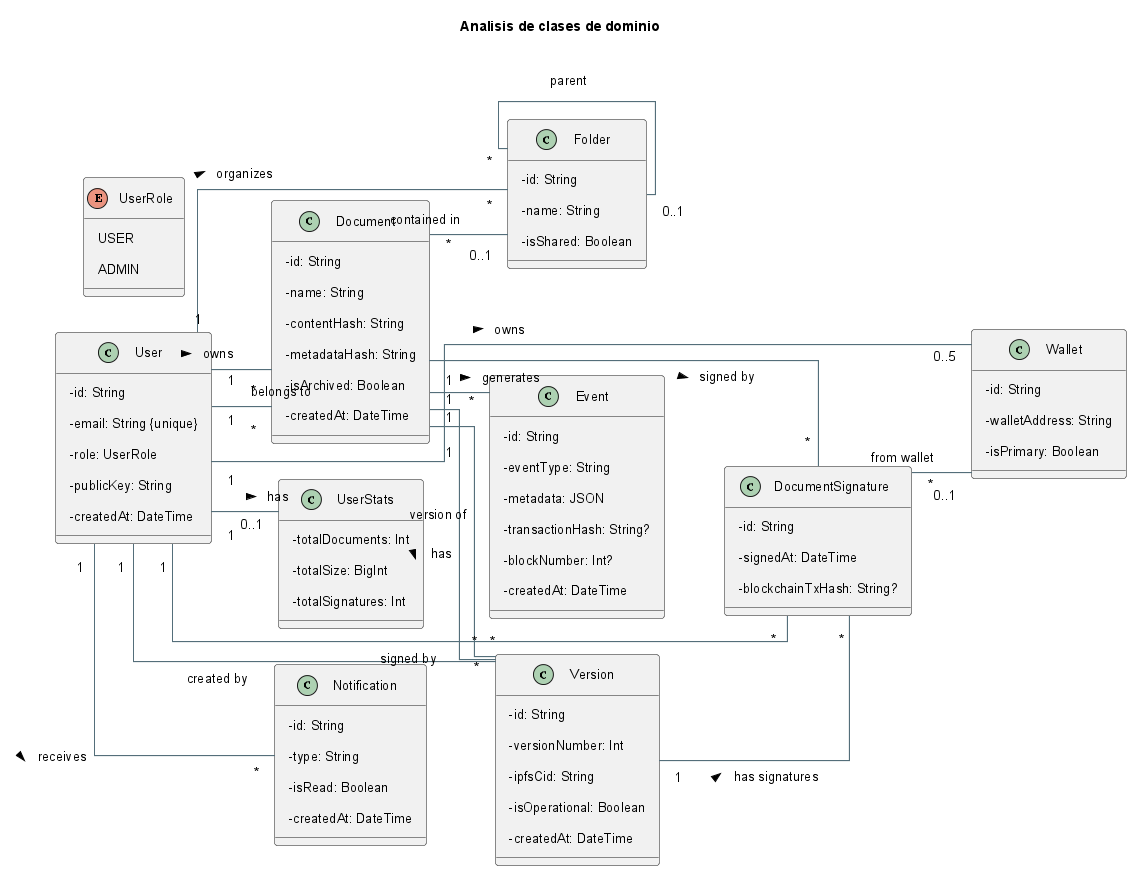
\includegraphics[width=0.9\textwidth]{diagramas/class-analysis.png}
    \caption{Diagrama de clases de análisis completo}
    \label{fig:class-analysis}
\end{figure}

\subsection{Estructuras de archivo y bases de datos}

El modelo de datos de DocumentChain comprende 17 tablas en PostgreSQL, organizadas en tres grupos funcionales:

\begin{itemize}
    \item \textbf{Entidades principales}: \texttt{users}, \texttt{wallets}, \texttt{documents}. Representan los actores y recursos centrales del sistema.
    \item \textbf{Entidades derivadas}: \texttt{versions}, \texttt{document\_signatures}, \texttt{folders}, \texttt{categories}, \texttt{events}. Modelan las operaciones y la organización jerárquica de documentos.
    \item \textbf{Entidades de soporte}: \texttt{sessions}, \texttt{notifications}, \texttt{user\_stats}, \texttt{document\_stats}, \texttt{system\_stats}, \texttt{notification\_preferences}, \texttt{email\_verifications}, \texttt{password\_resets}, \texttt{system\_config}. Cubren autenticación, auditoría, estadísticas y configuración.
\end{itemize}

Las relaciones clave son: un \texttt{user} puede tener múltiples \texttt{wallets}, \texttt{documents} y \texttt{sessions}; un \texttt{document} tiene múltiples \texttt{versions} y \texttt{document\_signatures}; los \texttt{events} registran toda la actividad auditada del sistema. La estructura completa, incluyendo las entidades blockchain e IPFS, se representa en el diagrama Entidad-Relación de la siguiente subsección.

\subsection{Diagrama Entidad-Relación}

El diagrama E-R muestra las relaciones entre las 17 tablas de la base de datos PostgreSQL. Las entidades principales son: \texttt{users}, \texttt{documents} y \texttt{wallets}; las entidades de relación incluyen \texttt{versions}, \texttt{document\_signatures}, \texttt{folders}, \texttt{categories} y \texttt{events}; las entidades de soporte son \texttt{sessions}, \texttt{notifications}, \texttt{user\_stats}, \texttt{document\_stats}, \texttt{system\_stats}, \texttt{notification\_preferences}, \texttt{email\_verifications}, \texttt{password\_resets} y \texttt{system\_config}.

\begin{figure}[H]
    \centering
    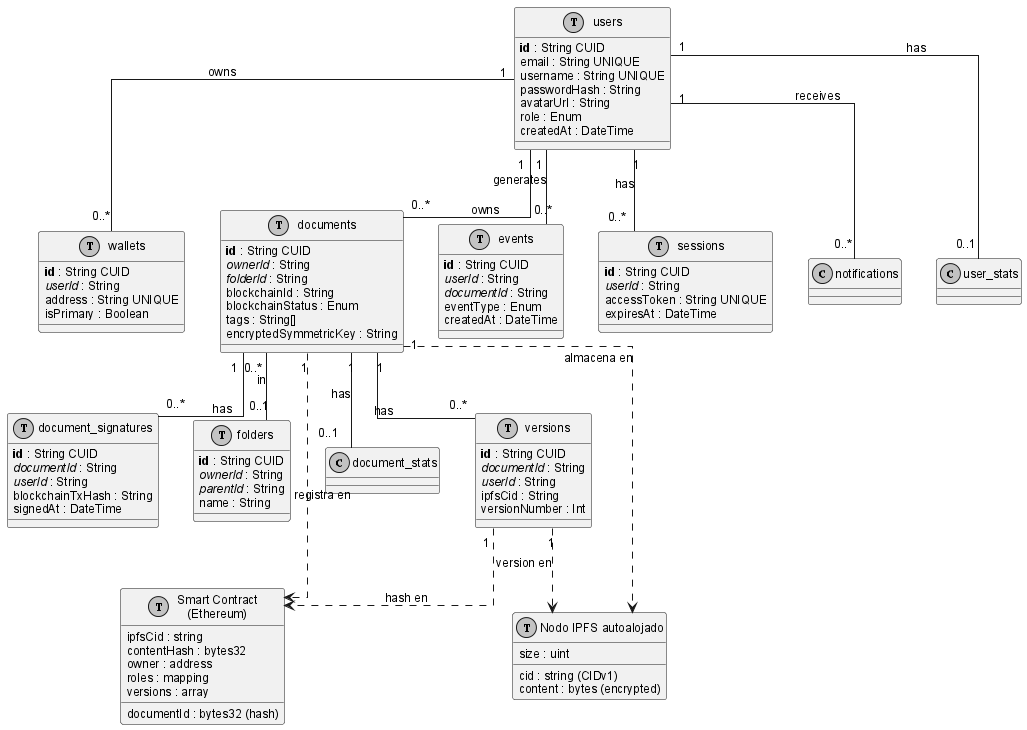
\includegraphics[width=0.9\textwidth]{diagramas/er-diagram.png}
    \caption{Diagrama Entidad-Relación de la base de datos}
    \label{fig:er-diagram}
\end{figure}

\subsection{Diagrama conjunto: base de datos y blockchain}

DocumentChain distribuye su información entre tres sistemas de persistencia complementarios: PostgreSQL, IPFS y Ethereum. En la arquitectura final no se consideran capas subordinadas entre sí, sino repositorios coordinados que operan al mismo nivel con responsabilidades diferentes. Por ello, el diagrama integrado representa conjuntamente tablas relacionales, referencias IPFS y estructuras \textit{on-chain} como elementos equivalentes dentro del modelo global de persistencia.

El diagrama siguiente muestra las correspondencias entre los tres repositorios, destacando las claves lógicas que enlazan el estado operativo con la verdad verificable registrada en blockchain:

\begin{itemize}
    \item \textbf{documents} $\leftrightarrow$ \textbf{Struct Document}: el campo \texttt{blockchainId} de PostgreSQL corresponde al identificador \texttt{docId} registrado en el contrato.
    \item \textbf{versions} $\leftrightarrow$ \textbf{Struct Version} $\leftrightarrow$ \textbf{IPFS CID}: el CID de cada versión enlaza simultáneamente el registro operativo, el contenido cifrado y la prueba inmutable de existencia.
    \item \textbf{document\_signatures} $\leftrightarrow$ \textbf{Struct Signature}: la firma operativa se almacena en PostgreSQL y se enlaza con el firmante \textit{on-chain} a través de la wallet asociada al usuario. La tabla conserva además una instantánea mínima de identidad (usuario mostrado y wallet usada) para seguir presentando el firmante en la interfaz aunque cambie el perfil o desaparezca la relación operativa original.
    \item \textbf{events} $\leftrightarrow$ \textbf{Mapping Permissions}: PostgreSQL conserva la evidencia operativa de concesiones, revocaciones y sincronización; el permiso activo y vigente se consulta en el mapping \texttt{DocumentRole} del contrato.
    \item \textbf{wallets} y \textbf{users} $\leftrightarrow$ \textbf{owner / roles}: las direcciones Ethereum enlazan la identidad operativa con la titularidad y los permisos on-chain.
\end{itemize}

La coexistencia de estos repositorios no constituye redundancia, sino separación de responsabilidades: PostgreSQL resuelve consulta y actualización operativa, IPFS preserva el contenido cifrado y Ethereum conserva la verdad verificable sobre propiedad, permisos, firmas y versiones. Las líneas discontinuas del diagrama marcan las correspondencias transversales entre estos tres dominios de persistencia.

\begin{figure}[H]
    \centering
    
\includegraphics[width=\linewidth]{diagramas/er-combined.png}
    \caption{Modelo integrado de persistencia: tablas PostgreSQL, referencias IPFS y estructuras/mappings del smart contract al mismo nivel}
    \label{fig:er-combined}
\end{figure}

\subsection{Persistencia coordinada: PostgreSQL, IPFS y blockchain}

El sistema utiliza tres mecanismos de persistencia complementarios, cada uno con responsabilidades bien diferenciadas y sin jerarquía conceptual entre ellos. La base de datos no sustituye a la blockchain, la blockchain no reemplaza a IPFS y IPFS no modela el estado operativo; juntos forman el subsistema de persistencia completo.

\subsubsection{Base de datos relacional (PostgreSQL)}

PostgreSQL almacena toda la información que requiere consultas relacionales eficientes y puede ser modificada con el tiempo:

\begin{itemize}
    \item \textbf{Datos de identidad}: cuentas de usuario, credenciales cifradas, configuración de perfil, preferencias de notificación.
    \item \textbf{Metadatos de documentos}: nombre, descripción, estado de blockchain (\textit{PREPARING / TX\_SUBMITTED / SYNCED}), referencia al CID de IPFS, visibilidad, \texttt{publicId} cuando aplica, y marcas de tiempo de creación y modificación.
    \item \textbf{Control de versiones}: historial de versiones por documento, referencia a cada CID en IPFS, autor y fecha de cada versión.
    \item \textbf{Estructura organizativa}: carpetas, categorías y la organización jerárquica de documentos.
    \item \textbf{Compartición y auditoría operativa}: eventos de preparación, confirmación y revocación, notificaciones y datos auxiliares para la interfaz y la trazabilidad interna.
    \item \textbf{Sesiones y auditoría interna}: tokens de sesión activos, registro de eventos de acceso, estadísticas de uso.
    \item \textbf{Estado de sincronización}: referencia al hash de transacción blockchain para cada documento/firma, facilitando la reconciliación de estados.
\end{itemize}

\subsubsection{Almacenamiento distribuido (backend IPFS compatible)}

La capa de almacenamiento IPFS compatible conserva el contenido binario de los archivos de forma direccionable por contenido y persistente:

\begin{itemize}
    \item \textbf{Contenido según visibilidad}: los documentos privados se cifran con AES-256-GCM antes de subirse a IPFS; los documentos públicos se almacenan en claro porque se exponen deliberadamente mediante enlace compartible.
    \item \textbf{Contenido inmutable}: cada versión de un archivo genera un CID (Content Identifier) único derivado del hash SHA-256 de su contenido. Ningún CID puede modificarse una vez generado.
    \item \textbf{Alta disponibilidad}: el sistema puede apoyarse en un proveedor gestionado como Pinata o en un clúster IPFS autoalojado cuando se requiere replicación local y control de nodos.
    \item El CID generado por IPFS se almacena en PostgreSQL y se registra en la blockchain, creando el puente entre los tres sistemas de persistencia.
\end{itemize}

\subsubsection{Blockchain (Smart Contract en Ethereum)}

La blockchain actúa como registro inmutable e infalsificable para operaciones de alta criticidad:

\begin{itemize}
    \item \textbf{Prueba de existencia de documentos}: para cada documento creado o nueva versión, el smart contract almacena el CID de IPFS, el hash del archivo, el identificador del propietario y la marca de tiempo. Estos datos no pueden alterarse ni eliminarse.
    \item \textbf{Registro de firmas digitales}: cada firma de documento queda inmutablemente registrada en la blockchain con la dirección Ethereum del firmante, el CID del documento firmado y la fecha/hora de la firma verificable criptográficamente.
    \item \textbf{Trazabilidad de propiedad}: el smart contract mantiene el histórico de transferencias de propiedad de documentos.
    \item \textbf{Validación independiente}: cualquier tercero puede verificar la autenticidad e integridad de un documento consultando directamente la blockchain, sin depender del sistema central.
    \item La blockchain NO almacena el contenido de los archivos (prohibitivo en coste y tamaño), sino únicamente las referencias (CIDs) y los hashes como prueba criptográfica.
\end{itemize}

\subsubsection{Estructuras de datos del smart contract}

El contrato \texttt{DocumentRegistry.sol} organiza sus datos en tres \textit{structs} principales, varios \textit{mappings} anidados y un sistema de roles granulares. A continuación se describe cada estructura:

\paragraph{Tipos y roles}

El contrato define un tipo enumerado \texttt{DocumentRole} para expresar el nivel de acceso de cada usuario a un documento:

\begin{itemize}
    \item \texttt{NONE} (0): sin acceso al documento.
    \item \texttt{VIEWER} (1): solo lectura; puede descargar y verificar firmas.
    \item \texttt{EDITOR} (2): lectura y escritura; puede subir nuevas versiones.
    \item \texttt{OWNER} (3): control total; puede compartir, firmar, transferir y eliminar.
\end{itemize}

Adicionalmente, el sistema de control de acceso basado en roles (RBAC) de OpenZeppelin gestiona dos roles globales: \texttt{ADMIN\_ROLE} para administradores de la plataforma, y \texttt{OPERATOR\_ROLE} para operadores de sistema.

\paragraph{Struct Document}

Almacena los metadatos de cada documento registrado en la blockchain. El identificador principal es un \texttt{bytes32} derivado del UUID del documento en base de datos:

\begin{table}[H]
\centering
\begin{tabular}{|l|l|p{7cm}|}
\hline
\textbf{Campo} & \textbf{Tipo} & \textbf{Descripción} \\
\hline
\texttt{docId} & \texttt{bytes32} & Identificador único del documento (hash del UUID) \\
\hline
\texttt{owner} & \texttt{address} & Dirección Ethereum del propietario actual \\
\hline
\texttt{createdAt} & \texttt{uint256} & Marca de tiempo de creación (Unix, \textit{block.timestamp}) \\
\hline
\texttt{updatedAt} & \texttt{uint256} & Marca de tiempo de la última modificación \\
\hline
\texttt{currentVersion} & \texttt{uint256} & Número de la versión operativa activa \\
\hline
\texttt{latestVersion} & \texttt{uint256} & Número de la versión más reciente creada \\
\hline
\texttt{isArchived} & \texttt{bool} & Indica si el documento está archivado \\
\hline
\texttt{isDeleted} & \texttt{bool} & Eliminación lógica (los datos permanecen en blockchain) \\
\hline
\end{tabular}
\caption{Campos del struct Document en el smart contract}
\end{table}

\paragraph{Struct Version}

Cada versión de un documento queda registrada de forma inmutable con su referencia a IPFS y, cuando procede, la metadata criptográfica correspondiente:

\begin{table}[H]
\centering
\begin{tabular}{|l|l|p{7cm}|}
\hline
\textbf{Campo} & \textbf{Tipo} & \textbf{Descripción} \\
\hline
\texttt{versionNumber} & \texttt{uint256} & Número secuencial de la versión \\
\hline
\texttt{ipfsCid} & \texttt{string} & CID de IPFS del archivo almacenado (cifrado si es privado; en claro si es público) \\
\hline
\texttt{encryptedKeyHash} & \texttt{bytes32} & Hash de la clave de cifrado para verificación \\
\hline
\texttt{createdBy} & \texttt{address} & Dirección Ethereum del autor de la versión \\
\hline
\texttt{createdAt} & \texttt{uint256} & Marca de tiempo de la versión \\
\hline
\texttt{isOperational} & \texttt{bool} & Indica si es la versión activa del documento \\
\hline
\texttt{restoredFrom} & \texttt{uint256} & Versión origen si fue restaurada (0 si es nueva) \\
\hline
\end{tabular}
\caption{Campos del struct Version en el smart contract}
\end{table}

\paragraph{Struct Signature}

Registra de forma inmutable cada firma digital aplicada sobre una versión concreta de un documento:

\begin{table}[H]
\centering
\begin{tabular}{|l|l|p{7cm}|}
\hline
\textbf{Campo} & \textbf{Tipo} & \textbf{Descripción} \\
\hline
\texttt{signer} & \texttt{address} & Dirección Ethereum del firmante \\
\hline
\texttt{signature} & \texttt{bytes} & Firma criptográfica ECDSA en bytes \\
\hline
\texttt{message} & \texttt{string} & Mensaje o hash firmado \\
\hline
\texttt{comment} & \texttt{string} & Comentario opcional del firmante \\
\hline
\texttt{timestamp} & \texttt{uint256} & Marca de tiempo exacta de la firma \\
\hline
\end{tabular}
\caption{Campos del struct Signature en el smart contract}
\end{table}

\paragraph{Mappings de estado}

El contrato utiliza mappings anidados para asociar eficientemente documentos con sus versiones, firmas y permisos de acceso:

\begin{table}[H]
\centering
\small
\begin{tabular}{|p{6cm}|p{8cm}|}
\hline
\textbf{Mapping} & \textbf{Propósito} \\
\hline
\texttt{\_documents[docId]} & Recuperar el struct Document por identificador \\
\hline
\texttt{\_versions[docId][versionNum]} & Recuperar el struct Version de una versión concreta \\
\hline
\texttt{\_signatures[docId][versionNum]} & Array de firmas sobre una versión dada \\
\hline
\texttt{\_hasSigned[docId][versionNum][address]} & Evitar firmas duplicadas por direccion \\
\hline
\texttt{\_permissions[docId][address]} & Rol (NONE/VIEWER/EDITOR/OWNER) de cada usuario \\
\hline
\texttt{\_documentUsers[docId]} & Conjunto de direcciones con acceso al documento \\
\hline
\texttt{\_userDocuments[address]} & Conjunto de documentos accesibles para un usuario \\
\hline
\texttt{\_suspendedUsers[address]} & Indicador de suspensión administrativa de un usuario \\
\hline
\end{tabular}
\caption{Mappings principales del smart contract DocumentRegistry}
\end{table}

\paragraph{Modelo coordinado de verdad y operación}

La arquitectura de DocumentChain establece una separación de responsabilidades que puede resumirse como sigue: \textbf{PostgreSQL gestiona el estado operativo mutable, IPFS conserva el contenido binario de cada versión y la blockchain garantiza la verdad inmutable y verificable}. PostgreSQL puede actualizar registros, recalcular agregados o mantener estados transitorios; IPFS preserva el objeto identificado por su CID, cifrado en los documentos privados y expuesto en claro en los públicos; Ethereum fija la evidencia de propiedad, permisos, firmas, versiones y transferencias. Este reparto permite operar con eficiencia sin renunciar a la auditabilidad externa.

\subsubsection{Flujo de persistencia coordinado}

Cuando un usuario sube un documento, los tres sistemas actúan en secuencia:
\begin{enumerate}
    \item El usuario envía el archivo y la visibilidad seleccionada; el backend cifra el contenido si es privado o lo mantiene en claro si es público antes de subirlo a IPFS, obteniendo un CID único.
    \item El backend persiste el CID y los metadatos en PostgreSQL con estado \textit{PREPARING}, junto con la visibilidad y el \texttt{publicId} cuando corresponde.
    \item El usuario firma la transacción con su wallet conectada; el smart contract registra el CID y el hash en la blockchain.
    \item El event listener detecta el evento blockchain, actualiza el estado en PostgreSQL a \textit{SYNCED} con el hash de la transacción y el identificador blockchain generado.
\end{enumerate}

\section{Diseño arquitectónico}

\subsection{Arquitectura de capas}

DocumentChain implementa una arquitectura en capas con separación clara de responsabilidades:

\subsubsection{Capas del Sistema}

\begin{enumerate}
    \item \textbf{Capa de Presentación (Frontend)}
    \begin{itemize}
        \item Componentes React con diseño atómico
        \item Gestión de estado con Context API
        \item Lógica de cifrado/descifrado
        \item Interacción con la wallet conectada
        \item Consumo de API REST
    \end{itemize}
    
    \item \textbf{Capa de Aplicación (Backend API)}
    \begin{itemize}
        \item Controllers: manejo de peticiones HTTP
        \item Services: lógica de negocio
        \item Middleware: autenticación, validación, rate limiting
        \item Routers: enrutamiento de endpoints
    \end{itemize}
    
    \item \textbf{Capa de Dominio}
    \begin{itemize}
        \item Entidades del modelo de datos
        \item Reglas de negocio core
        \item Validaciones de dominio
    \end{itemize}
    
    \item \textbf{Capa de Infraestructura}
    \begin{itemize}
        \item Prisma ORM (acceso a PostgreSQL)
        \item Adaptador de proveedor IPFS
        \item Cliente Ethereum (ethers.js)
        \item Event Listeners blockchain
        \item Sistema de email
        \item WebSocket server
    \end{itemize}
    
    \item \textbf{Capa de Blockchain}
    \begin{itemize}
        \item Smart Contract DocumentRegistry
        \item Nodos Ethereum (Hardhat local / Sepolia testnet)
        \item Eventos on-chain
    \end{itemize}
    
    \item \textbf{Capa de Almacenamiento}
    \begin{itemize}
        \item Backend IPFS compatible (Pinata o clúster propio)
        \item PostgreSQL database
    \end{itemize}
\end{enumerate}

\subsubsection{Diagrama de paquetes}

\begin{figure}[H]
    \centering
    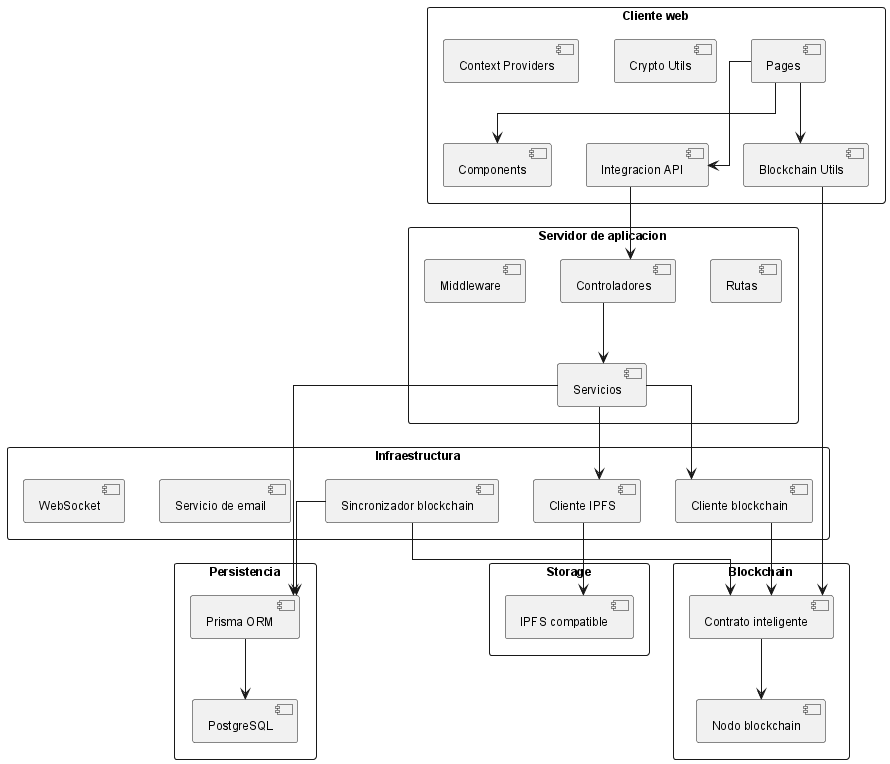
\includegraphics[width=0.9\textwidth]{diagramas/package-diagram.png}
    \caption{Diagrama de paquetes y dependencias}
    \label{fig:package-diagram}
\end{figure}

\subsection{Patrones de diseño aplicados}

\subsubsection{Prepare/Confirm Pattern (Transacciones Blockchain)}

\textbf{Problema}: Las transacciones blockchain requieren firma del usuario, creando un flujo asíncrono complejo.

\textbf{Solución}: Dividir la operación en dos fases:

\begin{enumerate}
    \item \textbf{Prepare}: Backend prepara todo (sube a IPFS, guarda en BD con estado PREPARING) y devuelve datos para transacción
    \item \textbf{Sign}: Frontend firma transacción con wallet del usuario
    \item \textbf{Confirm}: Frontend envía txHash al backend, que actualiza estado a TX\_SUBMITTED
    \item \textbf{Sync}: Event listener confirma cuando la transacción se mina y actualiza a SYNCED
\end{enumerate}

\textbf{Ventajas}:
\begin{itemize}
    \item No se pierde información si el usuario rechaza la firma
    \item Permite reintentos
    \item Estado siempre consistente
    \item Usuario mantiene control total
\end{itemize}

\begin{figure}[H]
    \centering
    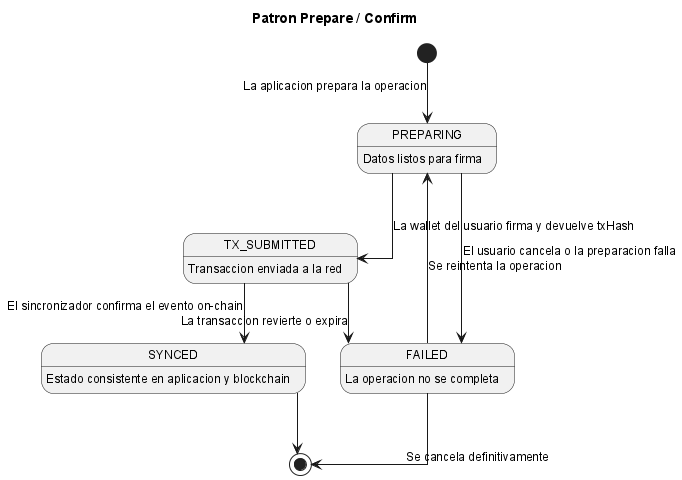
\includegraphics[width=0.9\textwidth]{diagramas/prepare-confirm.png}
    \caption{Diagrama del patrón Prepare/Confirm}
    \label{fig:prepare-confirm}
\end{figure}

\subsubsection{Repository Pattern}

\textbf{Problema}: Acoplamiento directo con la base de datos dificulta testing y cambios.

\textbf{Solución}: Prisma ORM act como Repository abstrayendo el acceso a datos.

\begin{itemize}
    \item Services solo dependen de la interfaz de Prisma
    \item Queries centralizadas y reutilizables
    \item Fácil mockeo para tests
\end{itemize}

\subsubsection{Service Layer Pattern}

\textbf{Problema}: Controllers con lógica de negocio complican reutilización y testing.

\textbf{Solución}: Controllers delgados que delegan en Services:

Los \textit{controllers} reciben las peticiones HTTP, validan los parámetros de entrada y delegan inmediatamente en la capa de servicios. Los \textit{services} concentran toda la lógica de negocio: validación de datos de dominio, orquestación de operaciones (cifrado, subida a IPFS, escritura en base de datos, preparación de transacciones blockchain), y actualización de estadísticas. Esta separación facilita el testing unitario de la lógica de negocio sin dependencias HTTP.

\subsubsection{Event-Driven Architecture}

Event listeners escuchan eventos del smart contract y sincronizan estado:

La arquitectura event-driven utiliza listeners que monitorizan el smart contract en tiempo real. Cuando ocurre un evento blockchain (por ejemplo, \textit{DocumentCreated}), el listener recupera la transacción pendiente en base de datos por su hash, actualiza el estado del documento a \textit{SYNCED} junto con el identificador blockchain asignado, actualiza las estadísticas del usuario propietario, y envía una notificación en tiempo real al cliente. Este mecanismo garantiza la consistencia entre el estado de la base de datos y el estado registrado en la blockchain.

\subsubsection{Circuit Breaker (Pausable Contract)}

El smart contract puede pausarse en emergencias:

El smart contract hereda de \texttt{Pausable} (OpenZeppelin), que proporciona las funciones \textit{pauseEmergency} y \textit{unpause}, restringidas al rol administrador mediante \textit{onlyAdmin}. Al pausar, se emite un evento \textit{SystemPaused} con el responsable y la marca de tiempo. El modificador \textit{whenNotPaused} protege todas las funciones críticas, rechazando operaciones durante el período de pausa. Este mecanismo permite reaccionar ante exploits o vulnerabilidades sin necesidad de redesplegar el contrato.

\subsection{Diagrama de clases de diseño}

El diagrama de clases de diseño incluye métodos, visibilidad y relaciones técnicas:

\begin{landscape}
\vspace*{\fill}
\centering
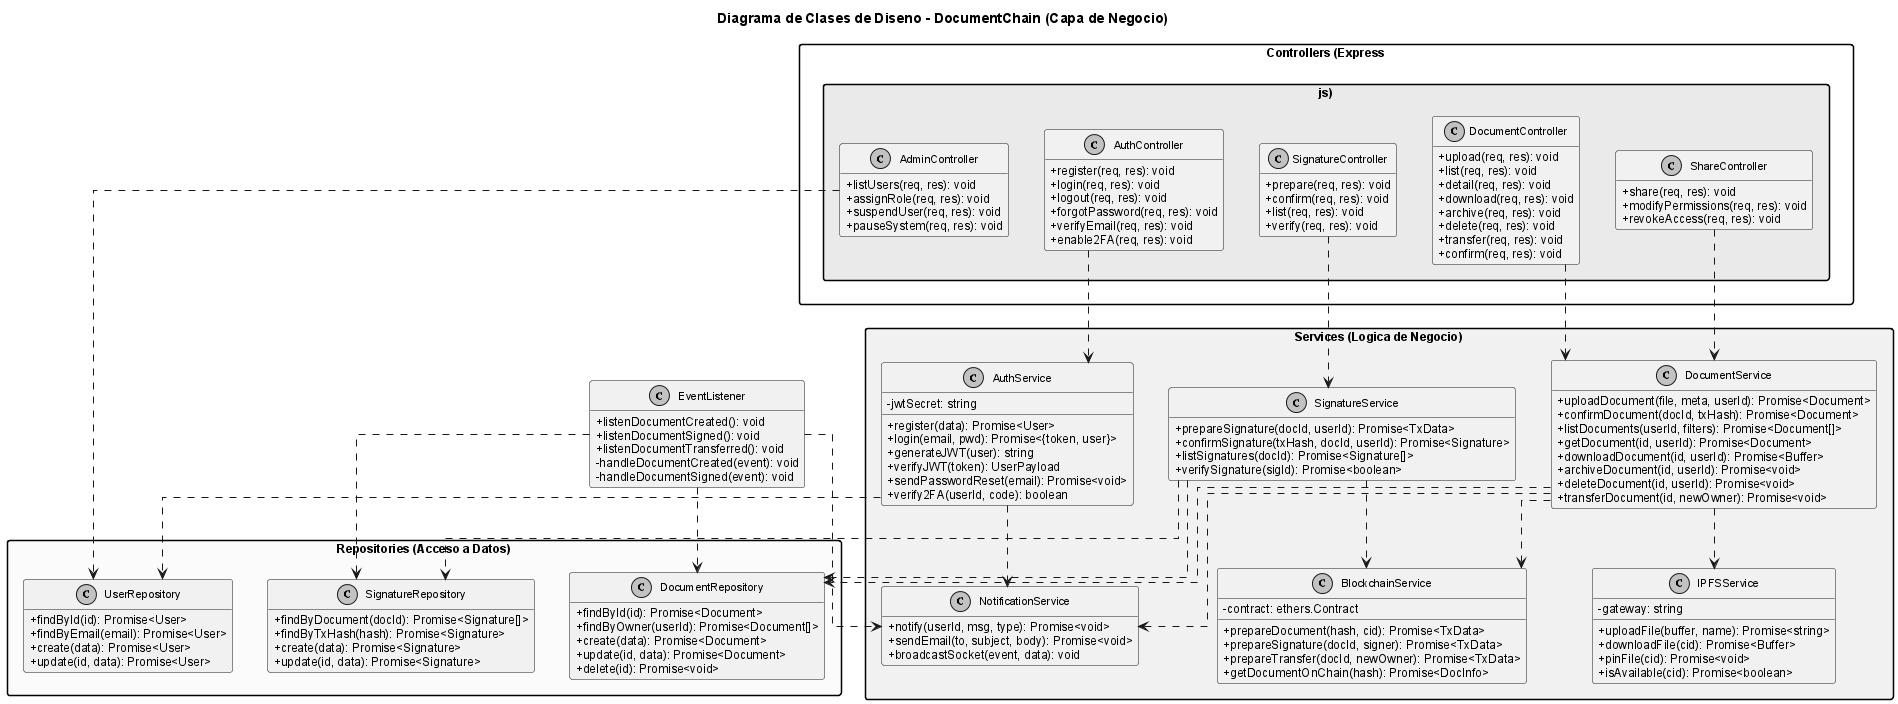
\includegraphics[width=0.95\linewidth]{diagramas/class-design.png}
\captionof{figure}{Diagrama de clases de diseño completo}
\label{fig:class-design}
\vspace*{\fill}
\end{landscape}

\subsubsection{Arquitectura del sistema por componentes}

El diagrama siguiente muestra la comunicación entre todos los módulos del sistema: el servidor API (Node.js + Express) concentra los Blockchain Event Listeners, los Routers, el Auth Middleware JWT+RBAC y la capa de Services. Los clientes acceden mediante HTTPS REST y WebSocket (Socket.IO). Las tres capas de persistencia son PostgreSQL (vía Prisma ORM), el Smart Contract en Ethereum y la capa de almacenamiento IPFS abstraída mediante proveedor configurable.

\begin{landscape}
\vspace*{\fill}
\centering
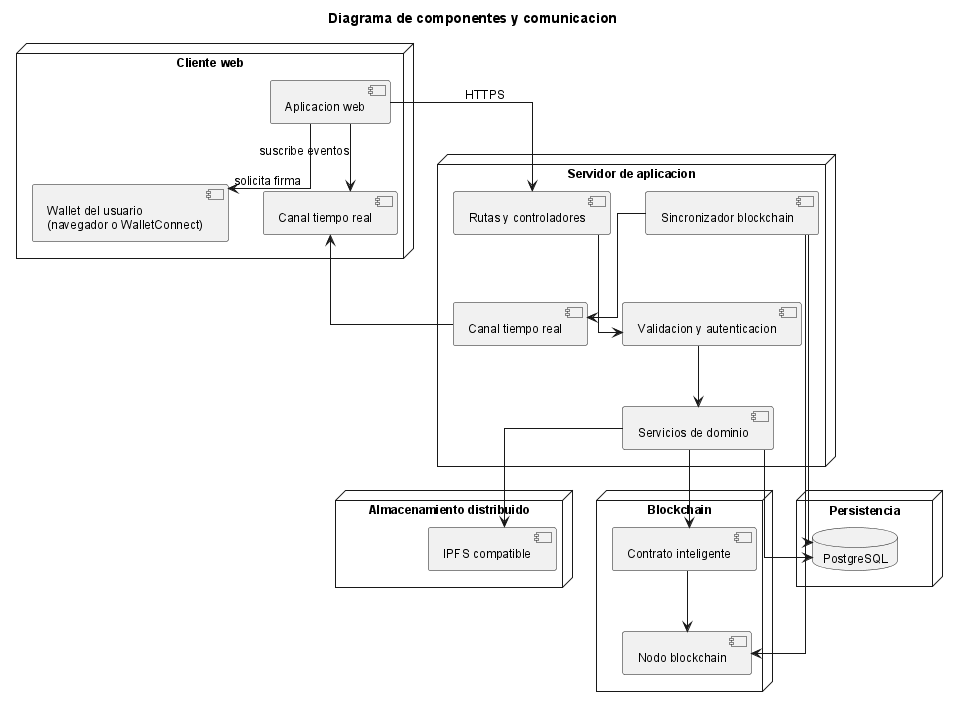
\includegraphics[width=0.76\linewidth]{diagramas/components.png}
\captionof{figure}{Diagrama de componentes y comunicación}
\label{fig:components}
\vspace*{\fill}
\end{landscape}

\section{Diseño de la interfaz}

\subsection{Representación de las interfaces del sistema}

La interfaz de DocumentChain se diseñó con los siguientes principios:

\begin{itemize}
    \item \textbf{Material Design adaptado}: Componentes reconocibles y predecibles
    \item \textbf{Responsive first}: Diseño móvil primero, escala a desktop
    \item \textbf{Accesibilidad}: Contraste WCAG AA, navegación por teclado
    \item \textbf{Feedback inmediato}: Loading spinners, toasts, progress bars
    \item \textbf{Tema oscuro/claro}: Respeta preferencias del sistema
\end{itemize}

\subsubsection{Componentes principales}

\begin{enumerate}
    \item \textbf{Layout Components}
    \begin{itemize}
        \item Navbar: navegación principal con logo, búsqueda, notificaciones, perfil
        \item Sidebar: navegación secundaria (carpetas, categorías, filtros)
        \item Footer: links de ayuda, versión, estado del sistema
    \end{itemize}
    
    \item \textbf{Document Components}
    \begin{itemize}
        \item DocumentCard: tarjeta con preview, metadata, acciones
        \item DocumentList: listado con paginación y sorting
        \item DocumentUploader: drag\&drop con progress y selector de visibilidad privada/pública
        \item DocumentViewer: modal de preview con acciones
        \item PublicDocumentPreview: previsualización inline de documentos públicos por tipo MIME
        \item PublicLinkActions: generación de enlace compartible y código QR
    \end{itemize}
    
    \item \textbf{Form Components}
    \begin{itemize}
        \item Input, Textarea, Select con validación
        \item FileInput con preview
        \item WalletConnector: punto de entrada para conectar una wallet compatible, incluyendo proveedores de navegador y WalletConnect v2 mediante código QR.
        \item PasswordStrengthIndicator
    \end{itemize}
    
    \item \textbf{Feedback Components}
    \begin{itemize}
        \item Toast: notificaciones temporales
        \item Modal: diálogos de confirmación
        \item LoadingSpinner: indicadores de carga
        \item ProgressBar: progreso de operaciones largas
    \end{itemize}
\end{enumerate}

\subsection{Prototipos de la interfaz de los componentes del sistema}

A continuación se incluyen capturas reales de las vistas principales implementadas en la versión final del sistema.

\subsubsection{Vista de inicio de sesión}

\begin{figure}[H]
    \centering
    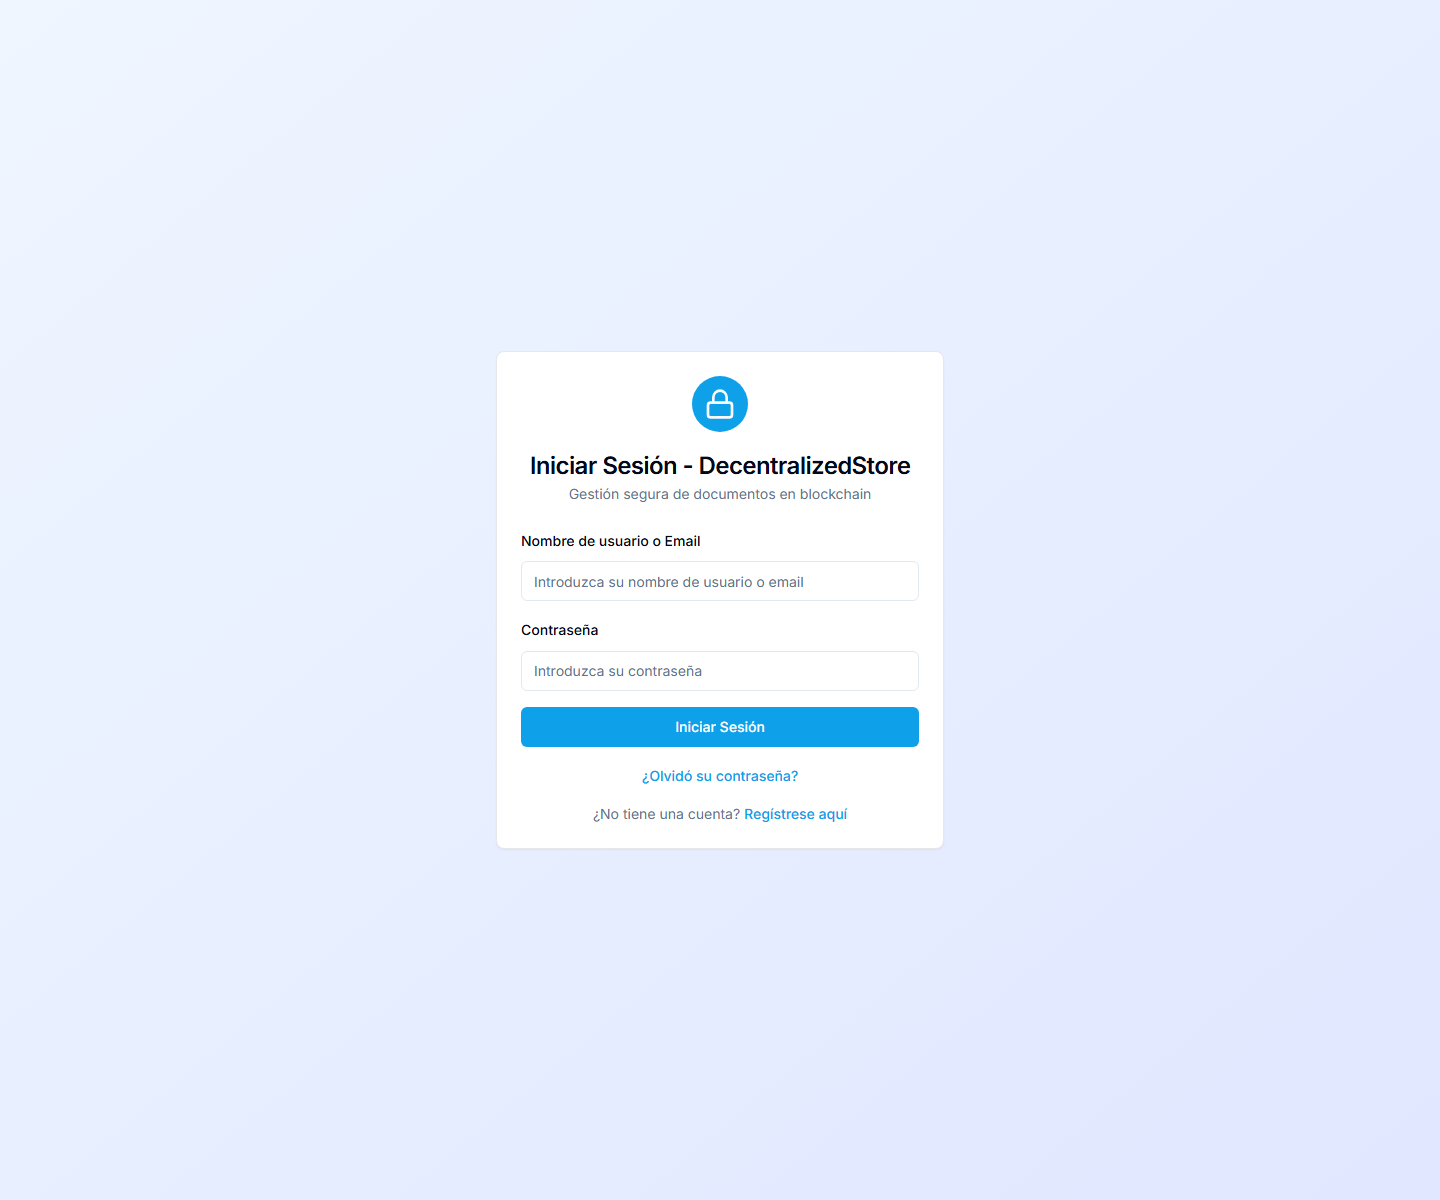
\includegraphics[width=0.72\textwidth]{capturas-ui/login-page.png}
    \caption{Pantalla de inicio de sesión}
    \label{fig:login}
\end{figure}

\textbf{Elementos}:
\begin{itemize}
    \item Formulario con nombre de usuario o email y contraseña.
    \item Recuperación de contraseña mediante enlace dedicado.
    \item Acceso al registro de nuevos usuarios.
    \item Segunda fase de verificación 2FA cuando la cuenta la requiere.
\end{itemize}

\subsubsection{Vista de registro}

\begin{figure}[H]
    \centering
    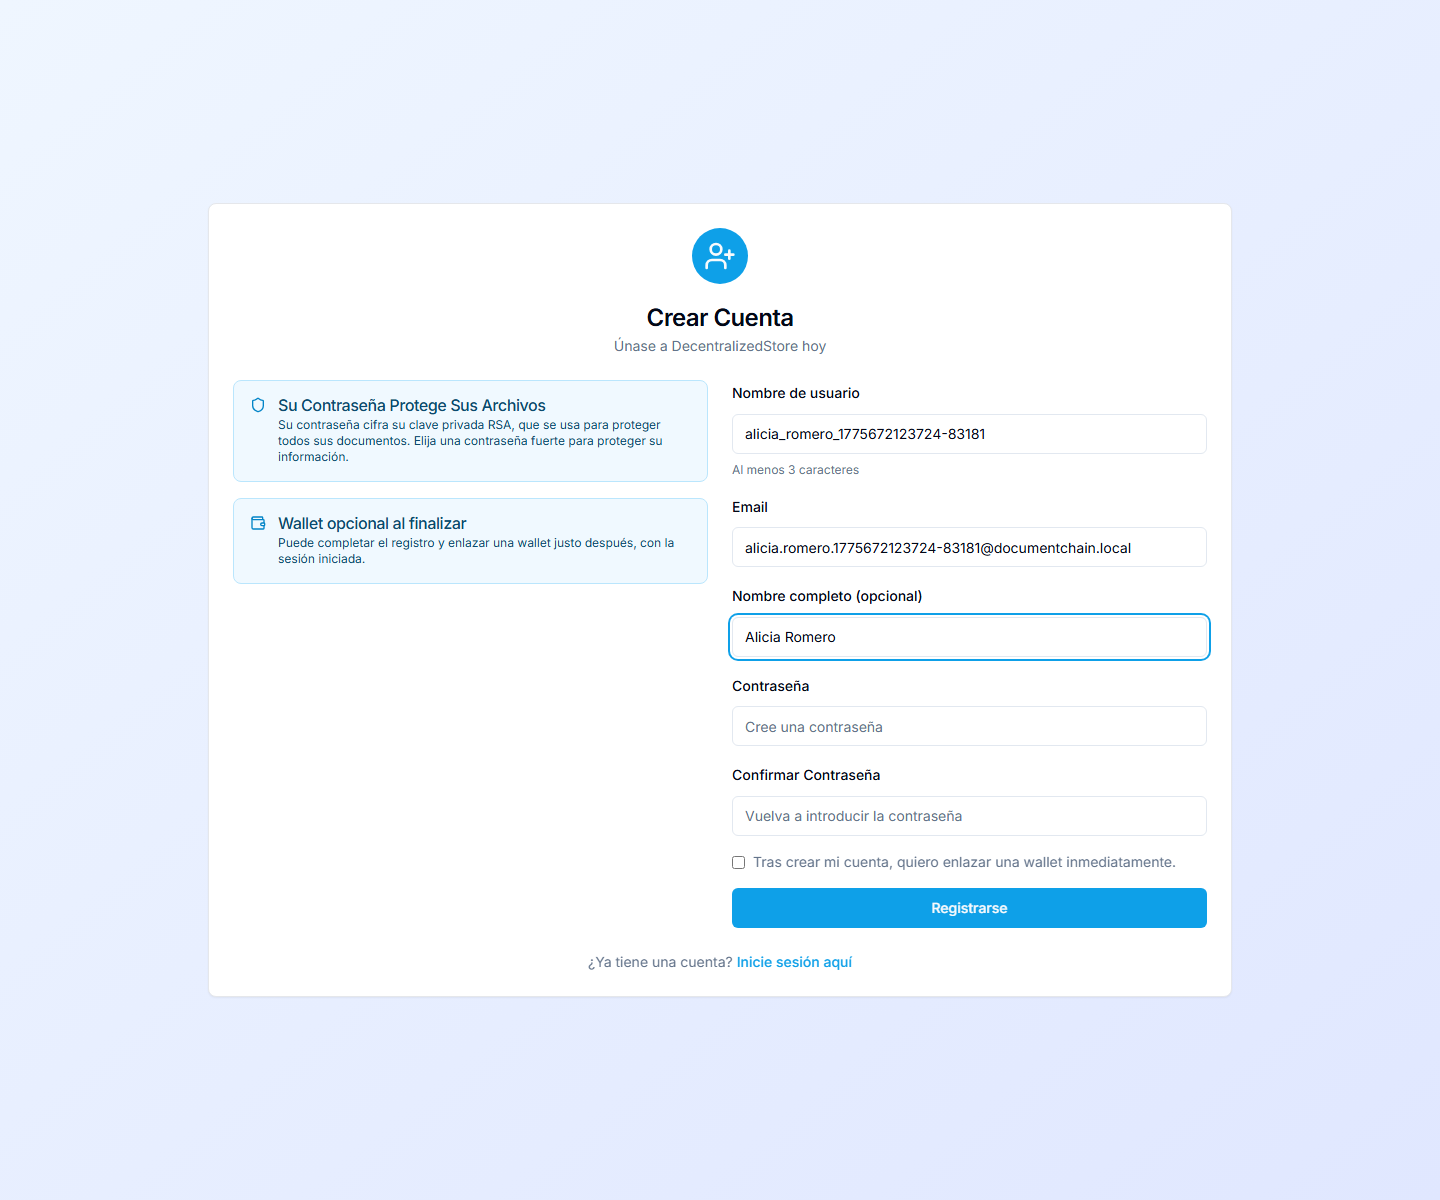
\includegraphics[width=0.72\textwidth]{capturas-ui/register-form.png}
    \caption{Pantalla de registro de usuario}
    \label{fig:register}
\end{figure}

\textbf{Elementos}:
\begin{itemize}
    \item Formulario con username, email, nombre completo opcional y doble confirmación de contraseña.
    \item Opción para continuar hacia el flujo de vinculación de wallet tras el alta.
    \item Continuación posterior mediante clave de recuperación y verificación de email.
\end{itemize}

\subsubsection{Vista principal de documentos}

\begin{figure}[H]
    \centering
    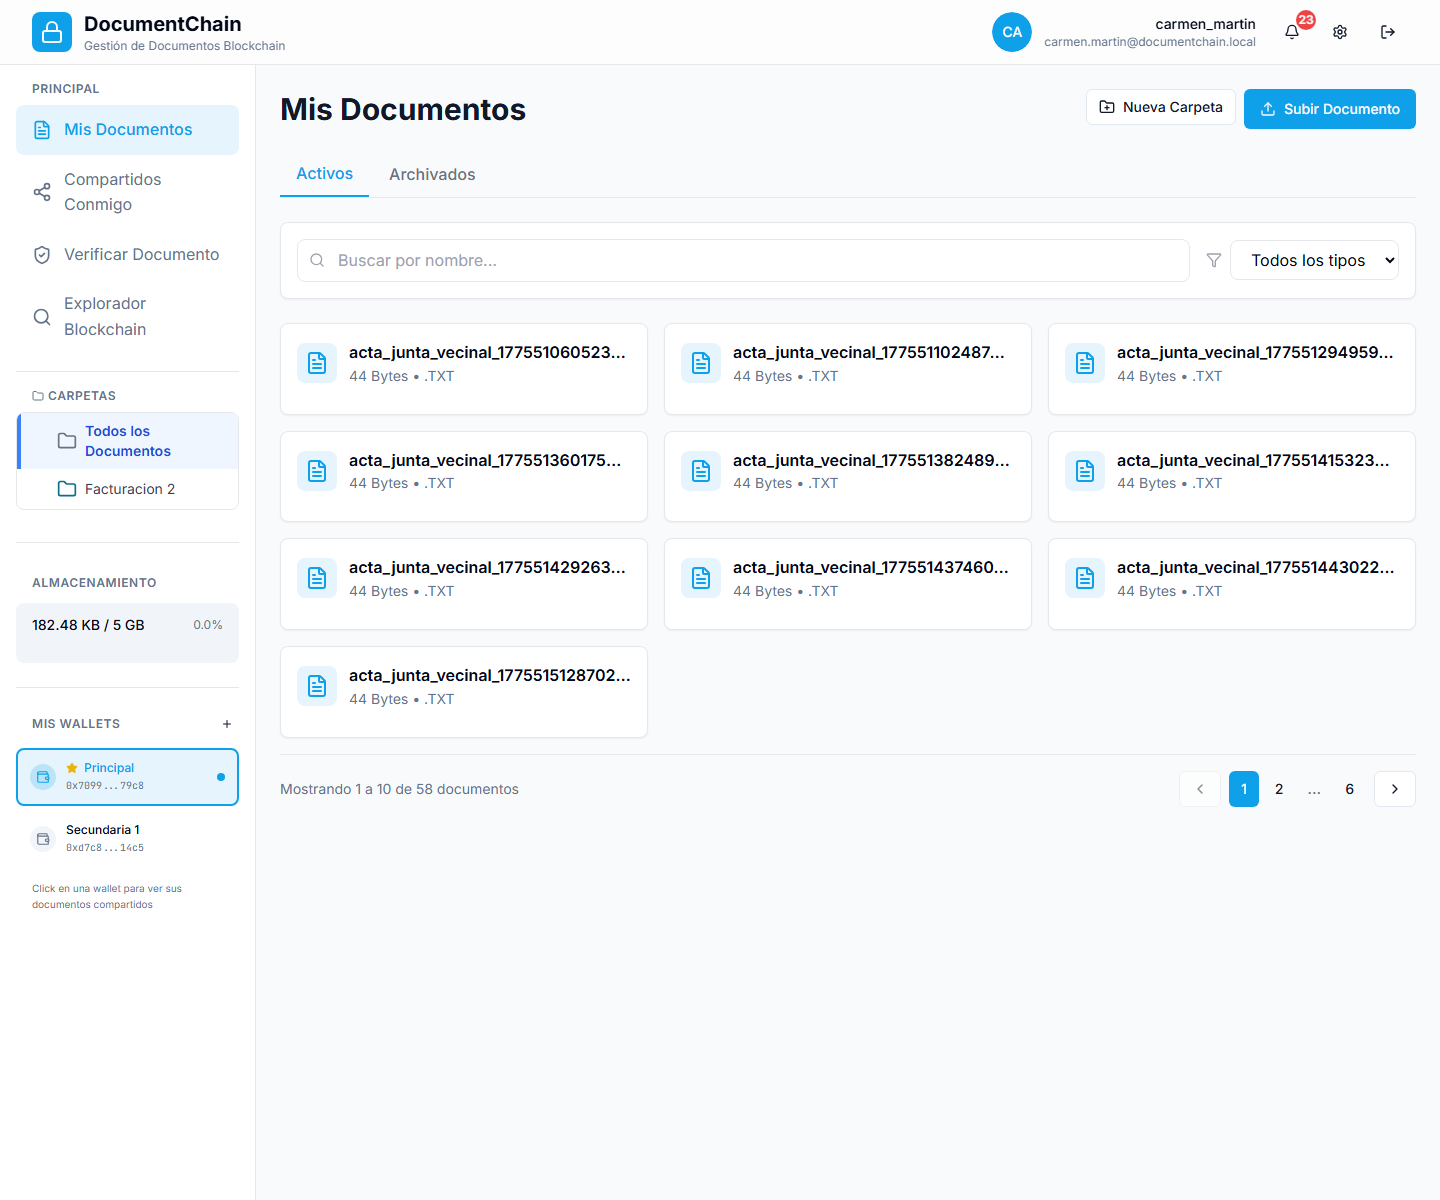
\includegraphics[width=0.94\textwidth]{capturas-ui/documents-page.png}
    \caption{Vista principal de documentos propios}
    \label{fig:dashboard}
\end{figure}

\textbf{Elementos}:
\begin{itemize}
    \item Barra lateral con accesos a documentos propios, compartidos, verificación y explorador blockchain.
    \item Zona superior con acciones de crear carpeta y subir documento.
    \item Filtros por texto, tipo de archivo y estado archivado.
    \item Listado paginado de documentos del usuario autenticado.
\end{itemize}

\subsubsection{Vista de detalle de documento}

\begin{figure}[H]
    \centering
    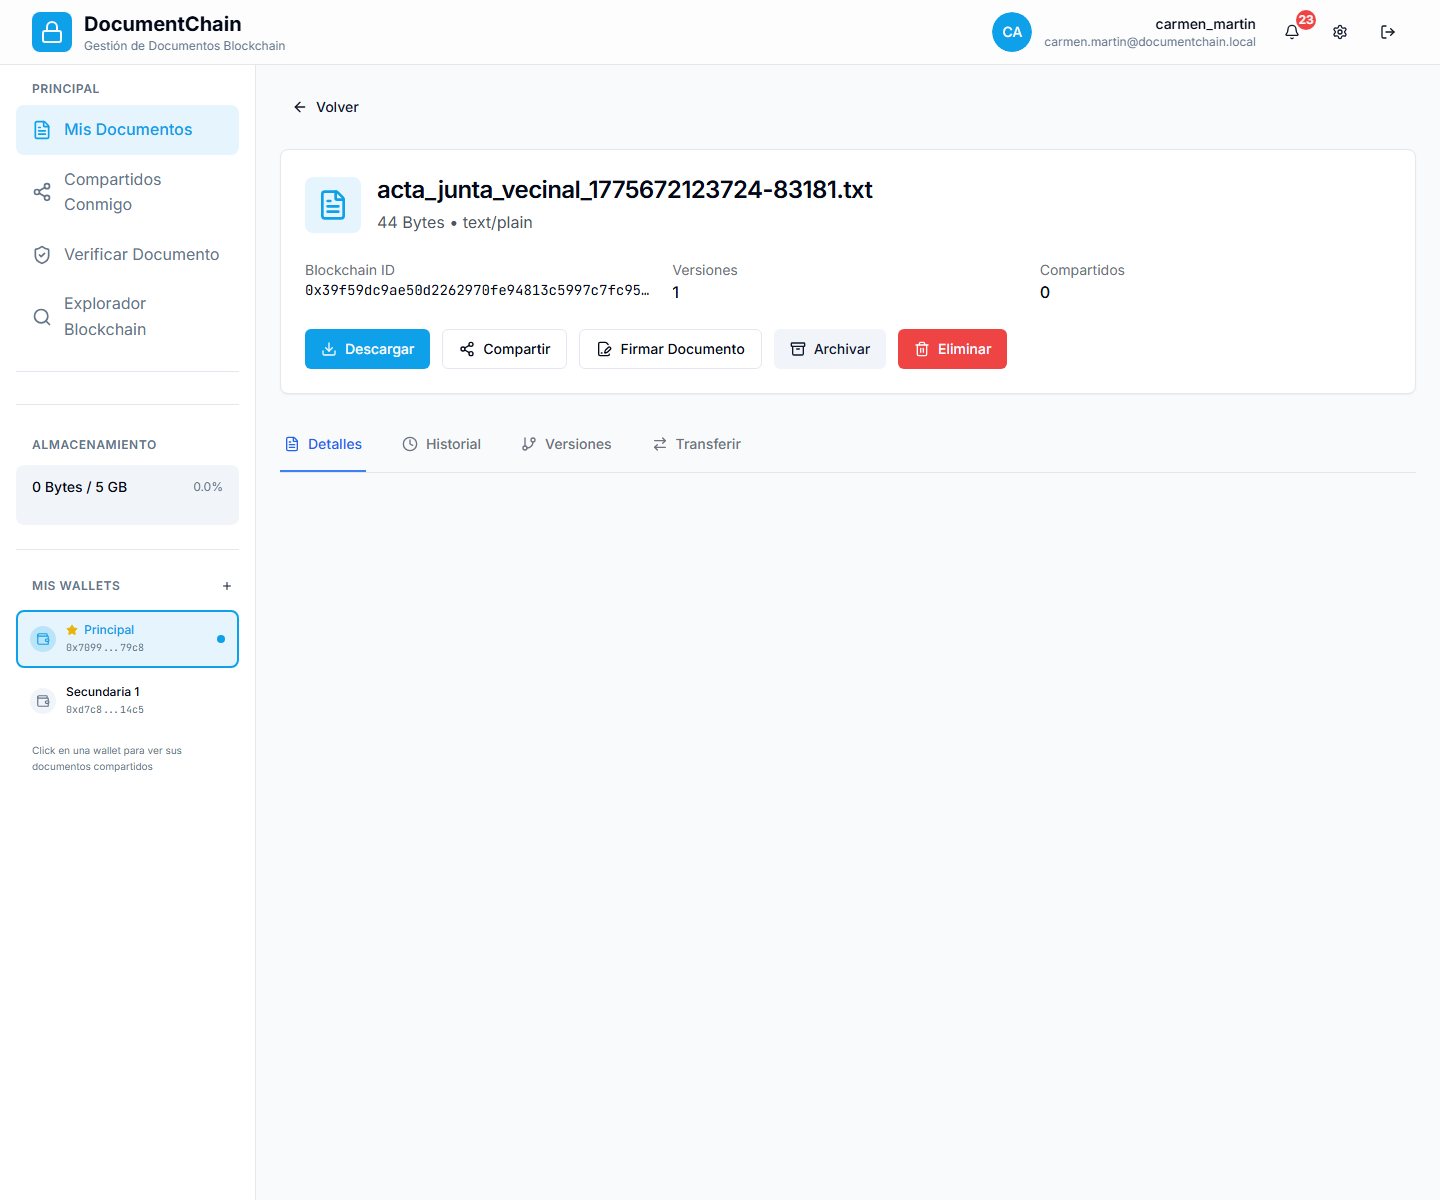
\includegraphics[width=0.94\textwidth]{capturas-ui/document-detail.png}
    \caption{Vista de detalle de documento}
    \label{fig:document-detail}
\end{figure}

\textbf{Elementos}:
\begin{itemize}
    \item Cabecera con metadatos esenciales, estado blockchain y acciones directas.
    \item Operaciones disponibles según rol: descargar, firmar, compartir, archivar, eliminar y transferir.
    \item En documentos públicos, acciones adicionales para copiar el enlace, abrir la página pública y generar el QR.
    \item Navegación por secciones internas: detalles, historial, versiones y transferencia para propietarios.
    \item En la sección de versiones, cada entrada puede abrir el modal de firmantes y mostrar un perfil reducido del firmante seleccionado sin exponer el perfil general de usuario.
    \item Listado de usuarios compartidos integrado en la propia vista cuando procede.
\end{itemize}

La consulta de firmantes se resuelve desde la propia vista de versiones. El frontend solicita las firmas de la versión seleccionada, el backend valida el acceso documental y devuelve una proyección acotada a nombre mostrado, alias disponible, wallet utilizada, estado de sincronización y referencia blockchain. Con ello se evita reutilizar el perfil general del usuario y se mantiene el principio de mínimo dato expuesto.

\subsubsection{Vista de compartir documento}

\begin{figure}[H]
    \centering
    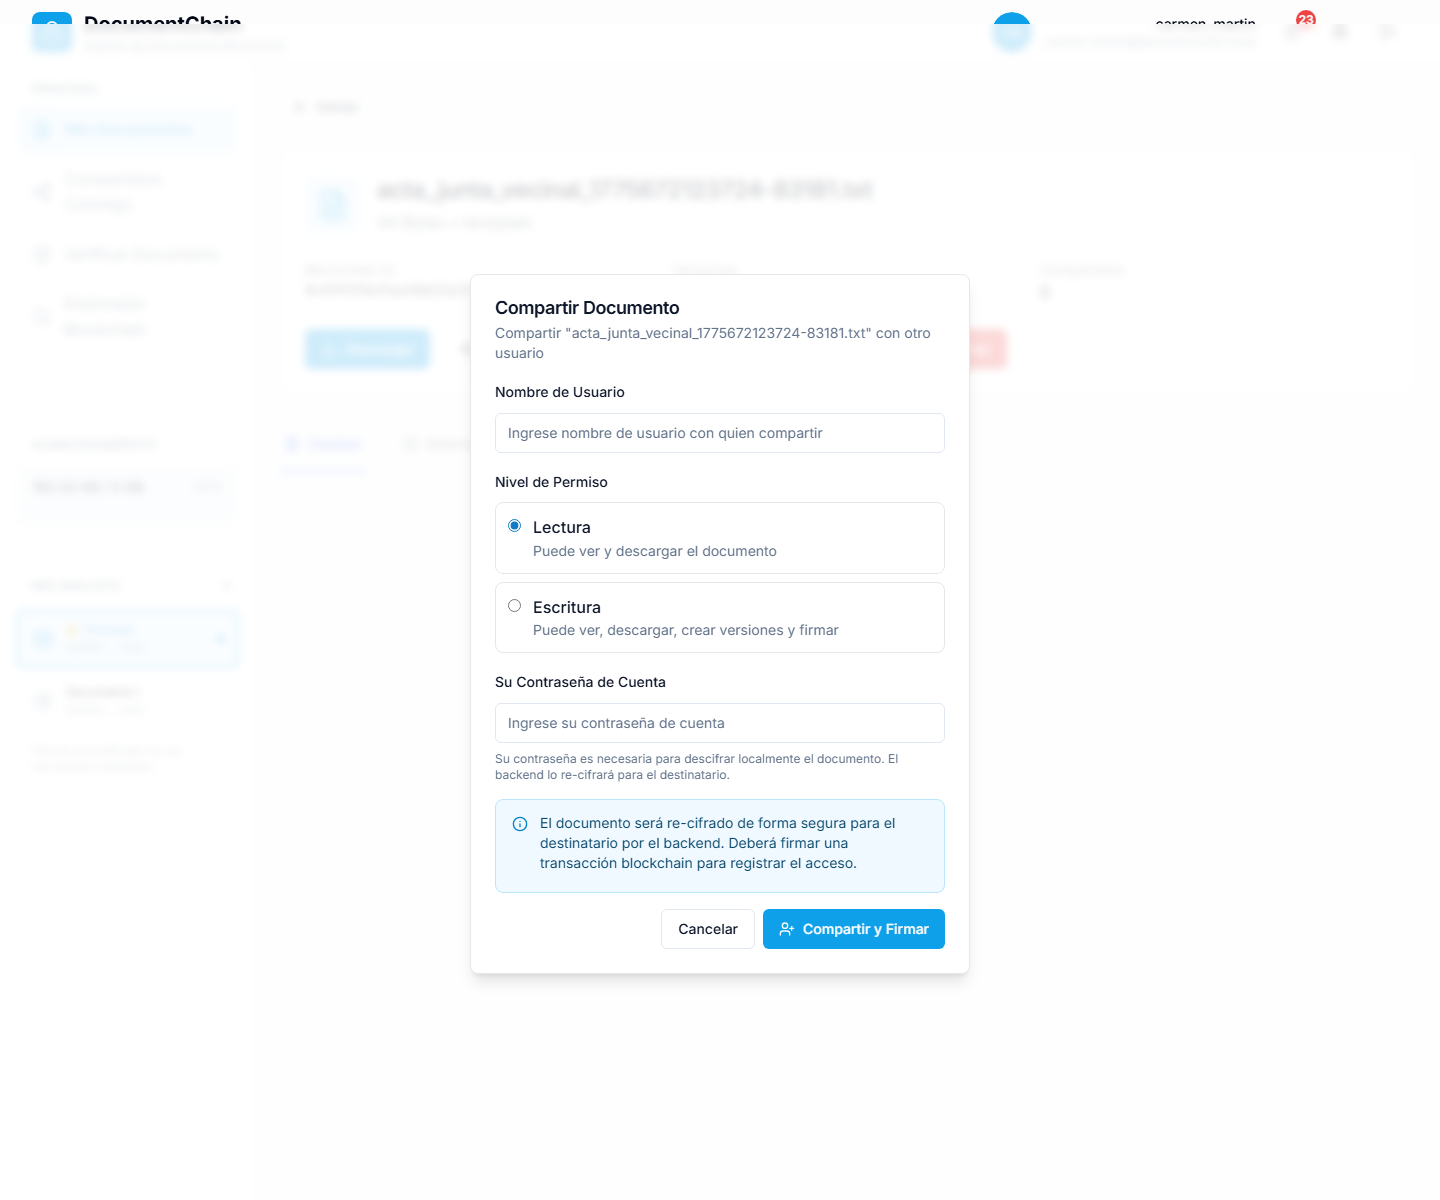
\includegraphics[width=0.76\textwidth]{capturas-ui/share-modal.png}
    \caption{Modal de compartir documento}
    \label{fig:share-modal}
\end{figure}

\textbf{Elementos}:
\begin{itemize}
    \item Búsqueda de usuario destino.
    \item Selección del nivel de permiso realmente soportado por el sistema.
    \item Confirmación con contraseña de cuenta y firma blockchain mediante wallet.
    \item Resumen del estado de compartición tras completarse la operación.
\end{itemize}

\subsubsection{Vista de documentos compartidos}

\begin{figure}[H]
    \centering
    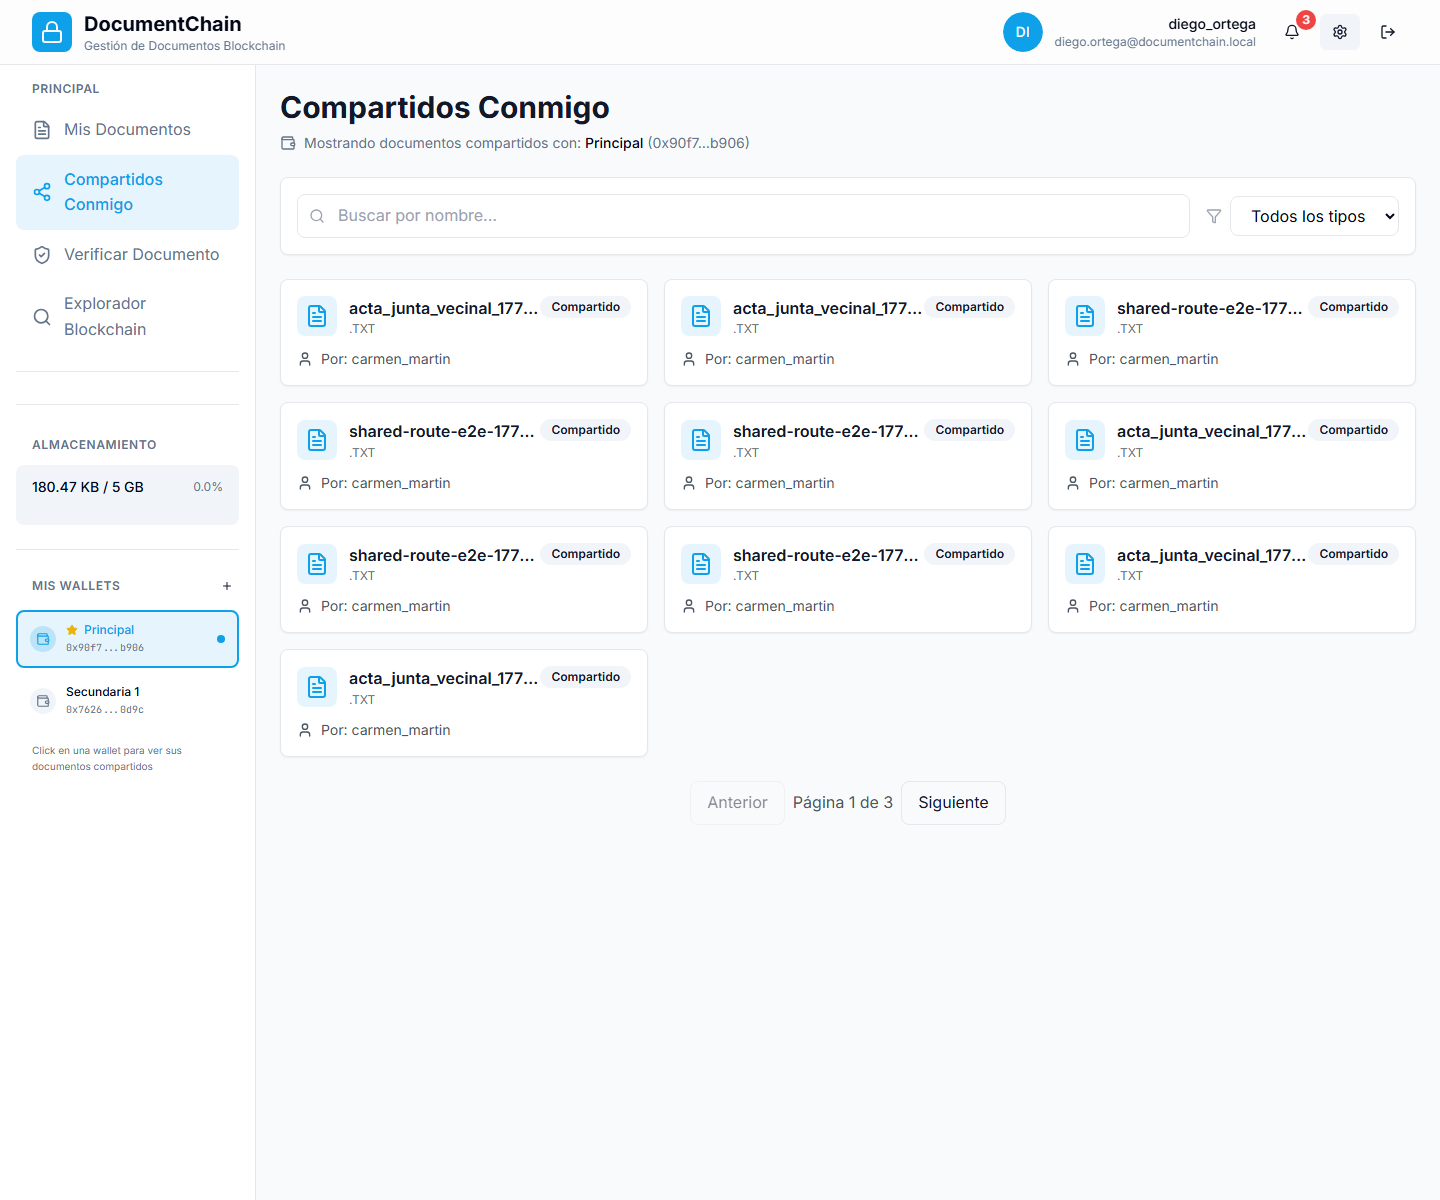
\includegraphics[width=0.94\textwidth]{capturas-ui/shared-page.png}
    \caption{Vista de documentos compartidos con el usuario}
    \label{fig:shared-documents-ui}
\end{figure}

\textbf{Elementos}:
\begin{itemize}
    \item Listado exclusivo de documentos recibidos mediante compartición.
    \item Indicador de wallet activa, relevante para resolver permisos recibidos on-chain.
    \item Filtros por nombre y tipo de archivo.
    \item Navegación al detalle del documento compartido conservando restricciones de rol.
\end{itemize}

\subsubsection{Vista de administración (Solo Admin)}

\begin{figure}[H]
    \centering
    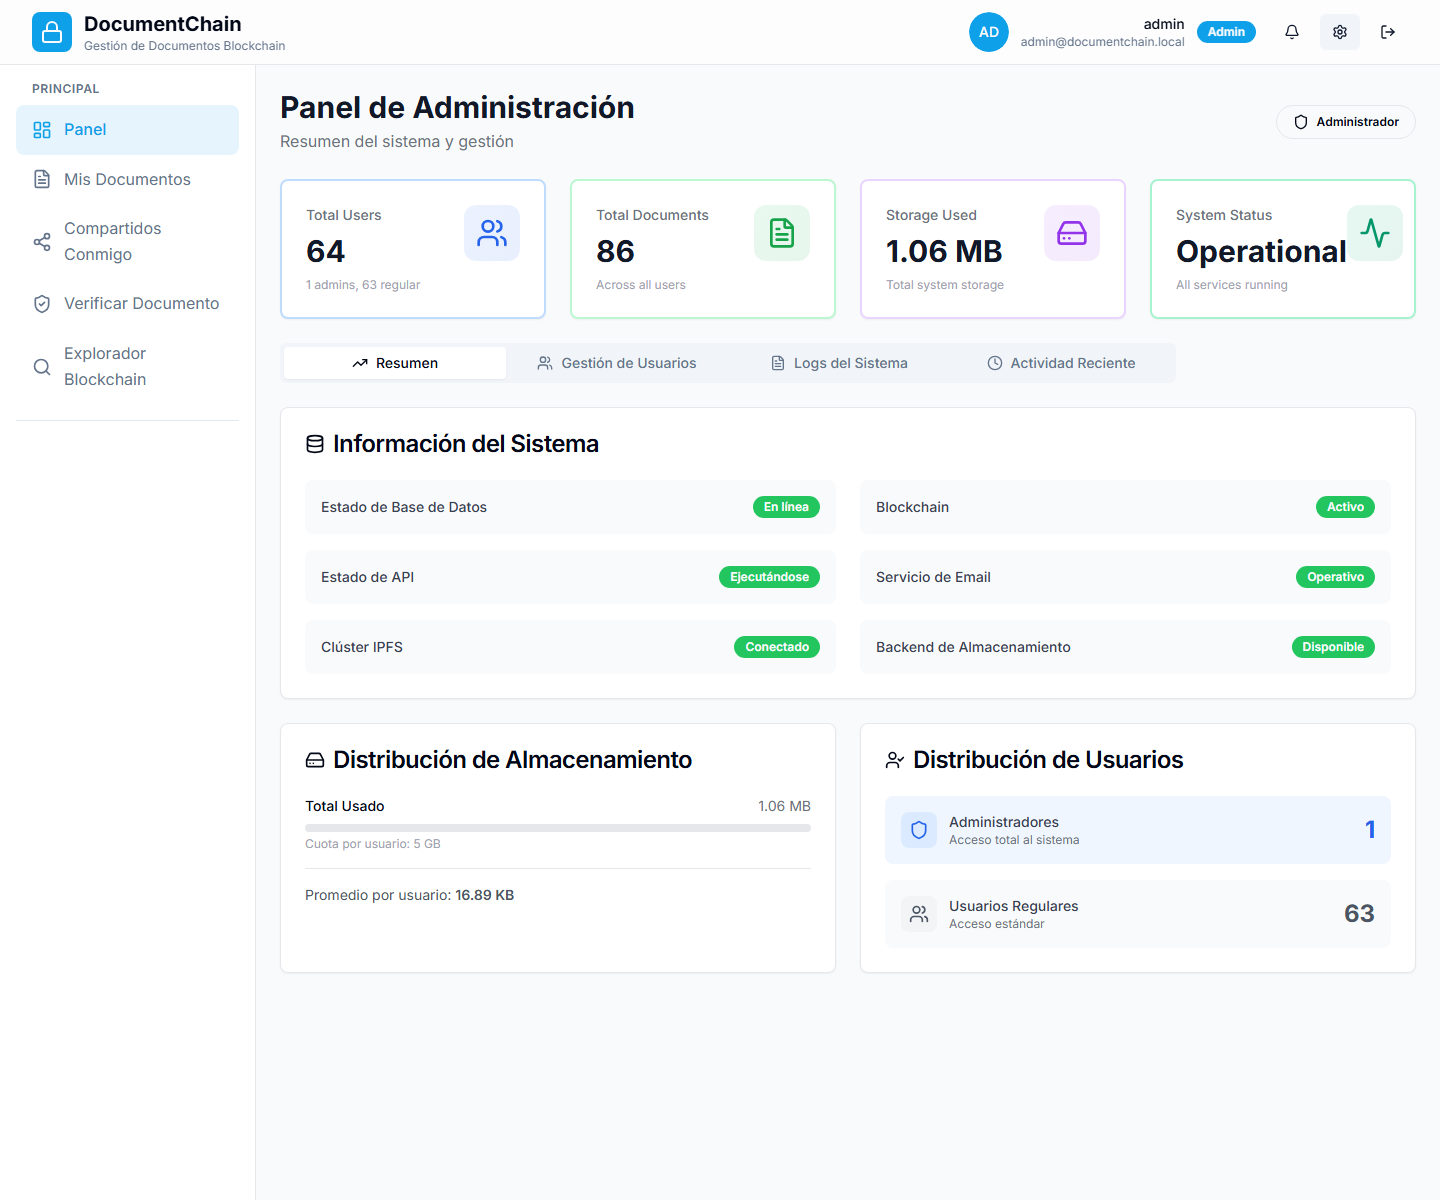
\includegraphics[width=0.94\textwidth]{capturas-ui/admin-dashboard.png}
    \caption{Panel de administración}
    \label{fig:admin-dashboard}
\end{figure}

\textbf{Elementos}:
\begin{itemize}
    \item Tarjetas de resumen con usuarios, documentos, almacenamiento y estado general.
    \item Paneles de salud de servicios para base de datos, API, IPFS y blockchain.
    \item Pestañas separadas para resumen, gestión de usuarios, logs del sistema y actividad reciente.
    \item Distribución de almacenamiento y usuarios sin recurrir a gráficas ficticias no implementadas.
\end{itemize}

\subsubsection{Vista de auditoría blockchain}

\begin{figure}[H]
    \centering
    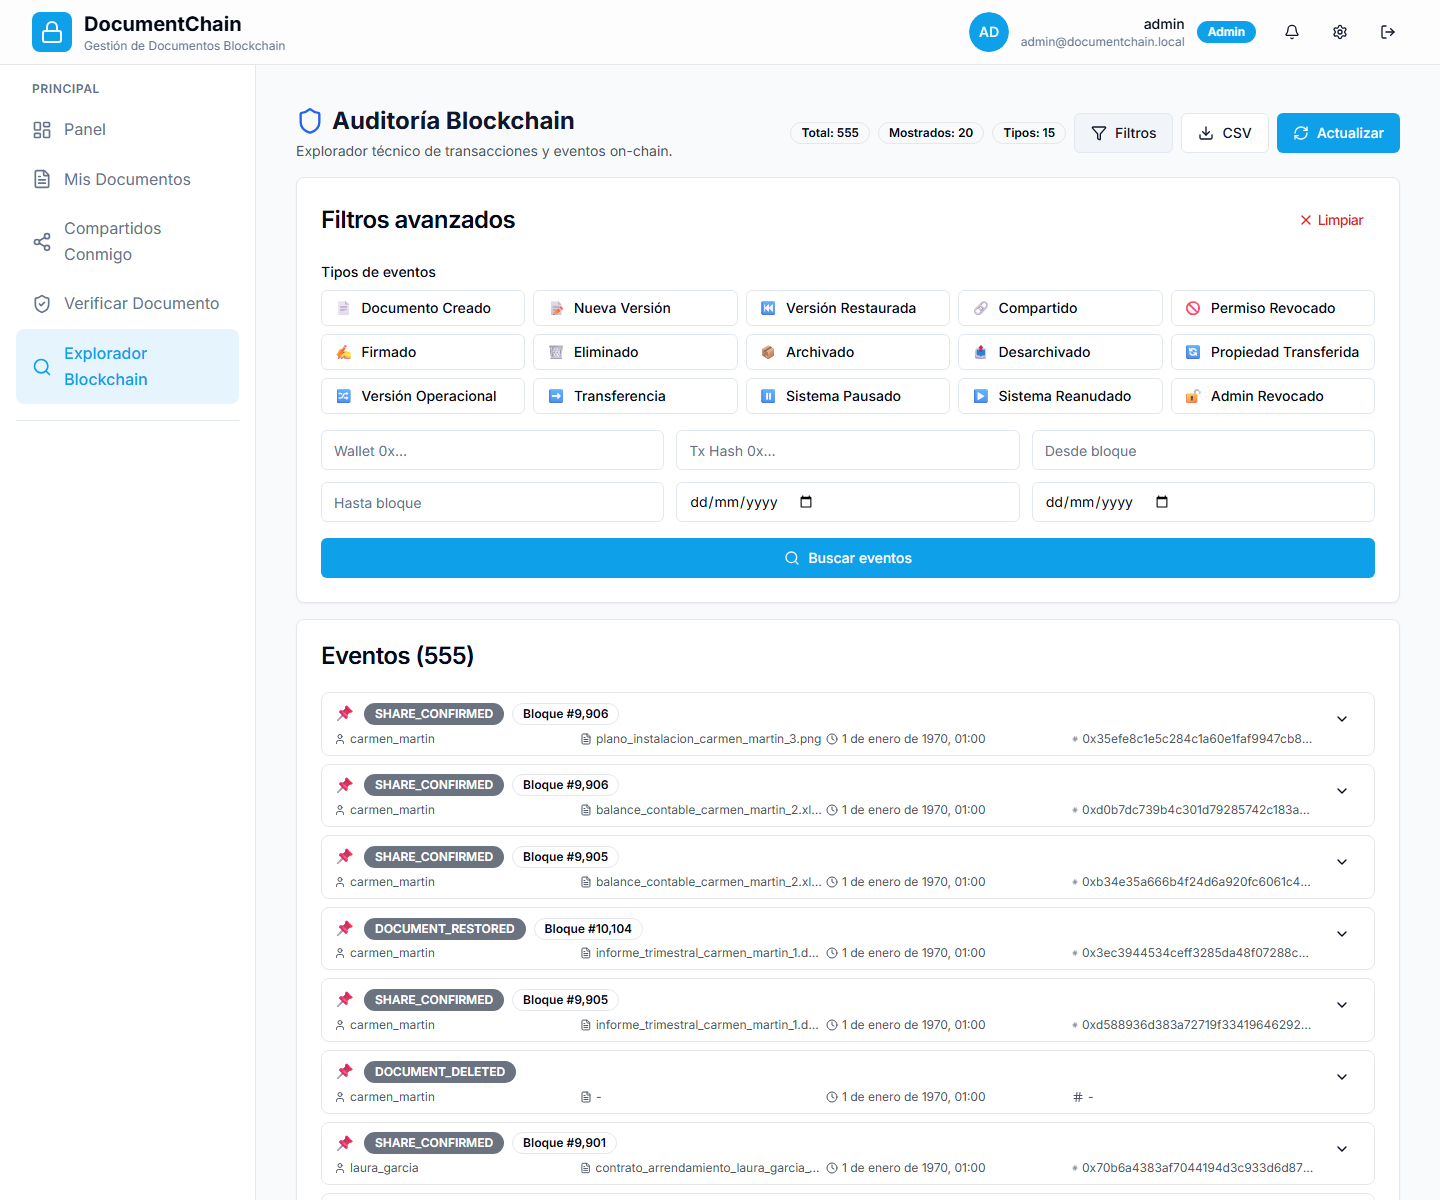
\includegraphics[width=0.94\textwidth]{capturas-ui/blockchain-auditor.png}
    \caption{Vista del auditor blockchain}
    \label{fig:blockchain-auditor}
\end{figure}

\textbf{Elementos}:
\begin{itemize}
    \item Filtros avanzados por tipo de evento, wallet, txHash, bloque y rango temporal.
    \item Resumen superior con número total, mostrados y tipos activos.
    \item Exportación CSV de eventos filtrados.
    \item Expansión de eventos para inspeccionar metadatos y referencias técnicas.
\end{itemize}

\subsubsection{Vista de verificación pública}

\begin{figure}[H]
    \centering
    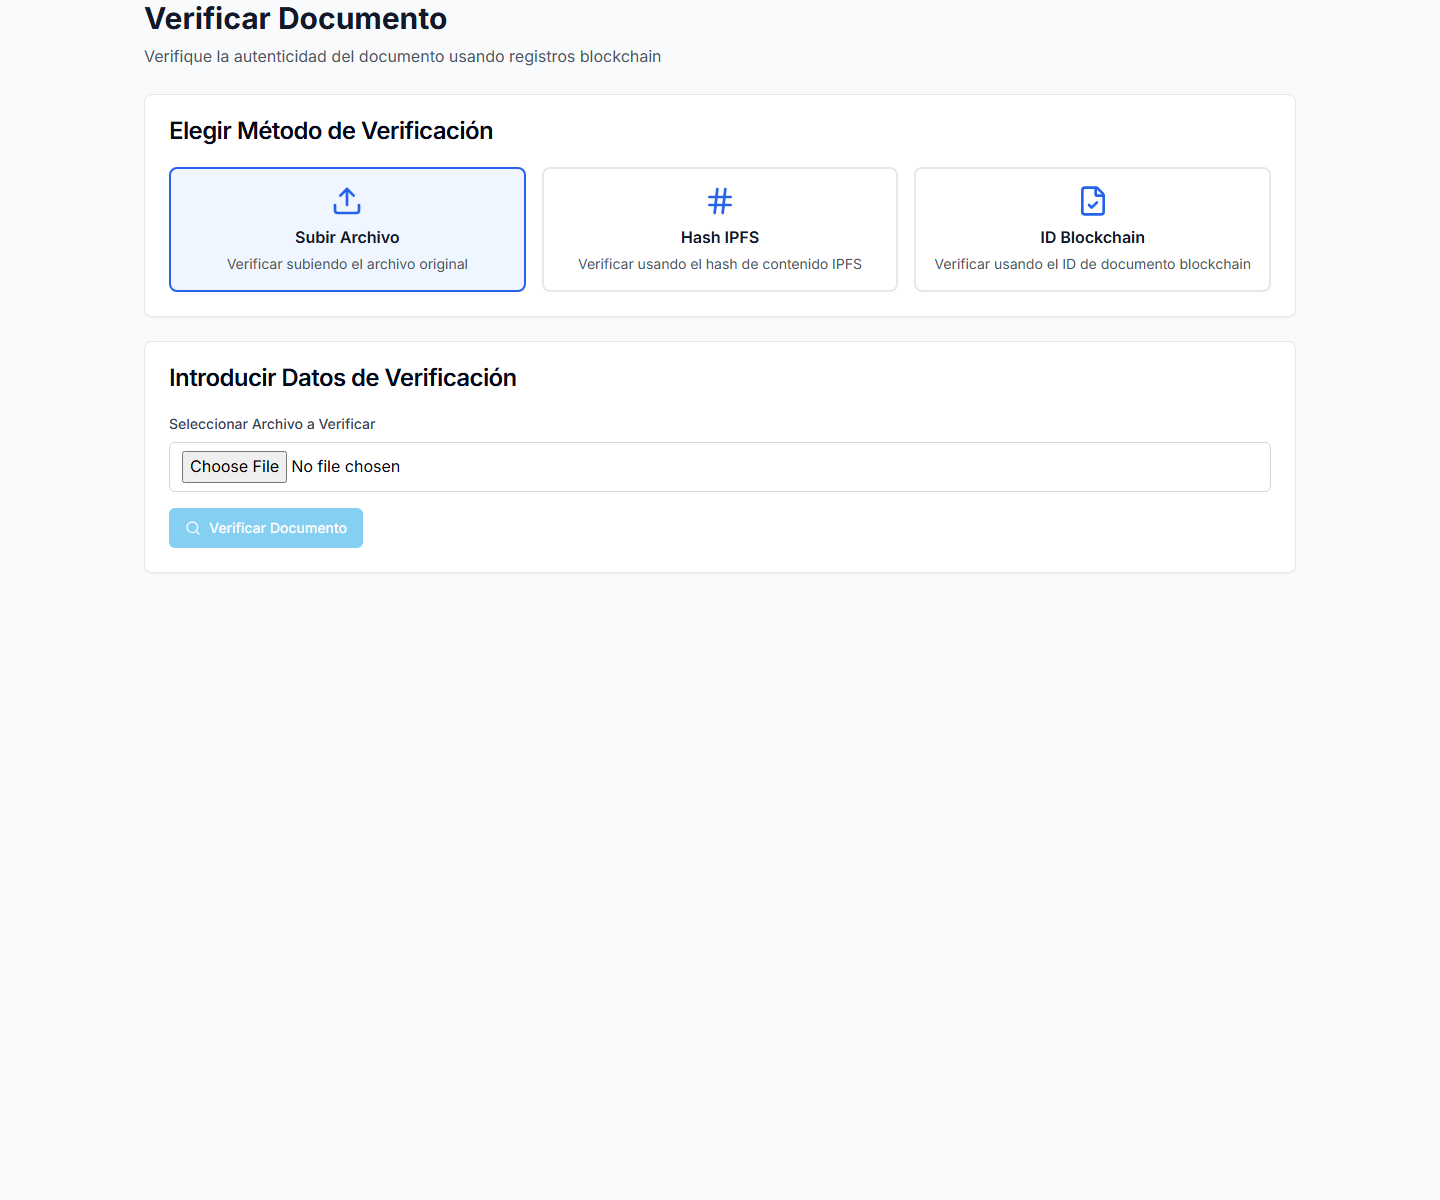
\includegraphics[width=0.9\textwidth]{capturas-ui/verify-page.png}
    \caption{Vista de verificación de autenticidad}
    \label{fig:verify-ui}
\end{figure}

\textbf{Elementos}:
\begin{itemize}
    \item Selección del método de verificación: archivo, CID IPFS o identificador blockchain.
    \item Formulario específico por método.
    \item Panel de resultados con existencia, integridad, propietario, versiones y firmas.
    \item Acceso público sin autenticación previa.
\end{itemize}

\subsubsection{Vista de perfil de usuario}

\begin{figure}[H]
    \centering
    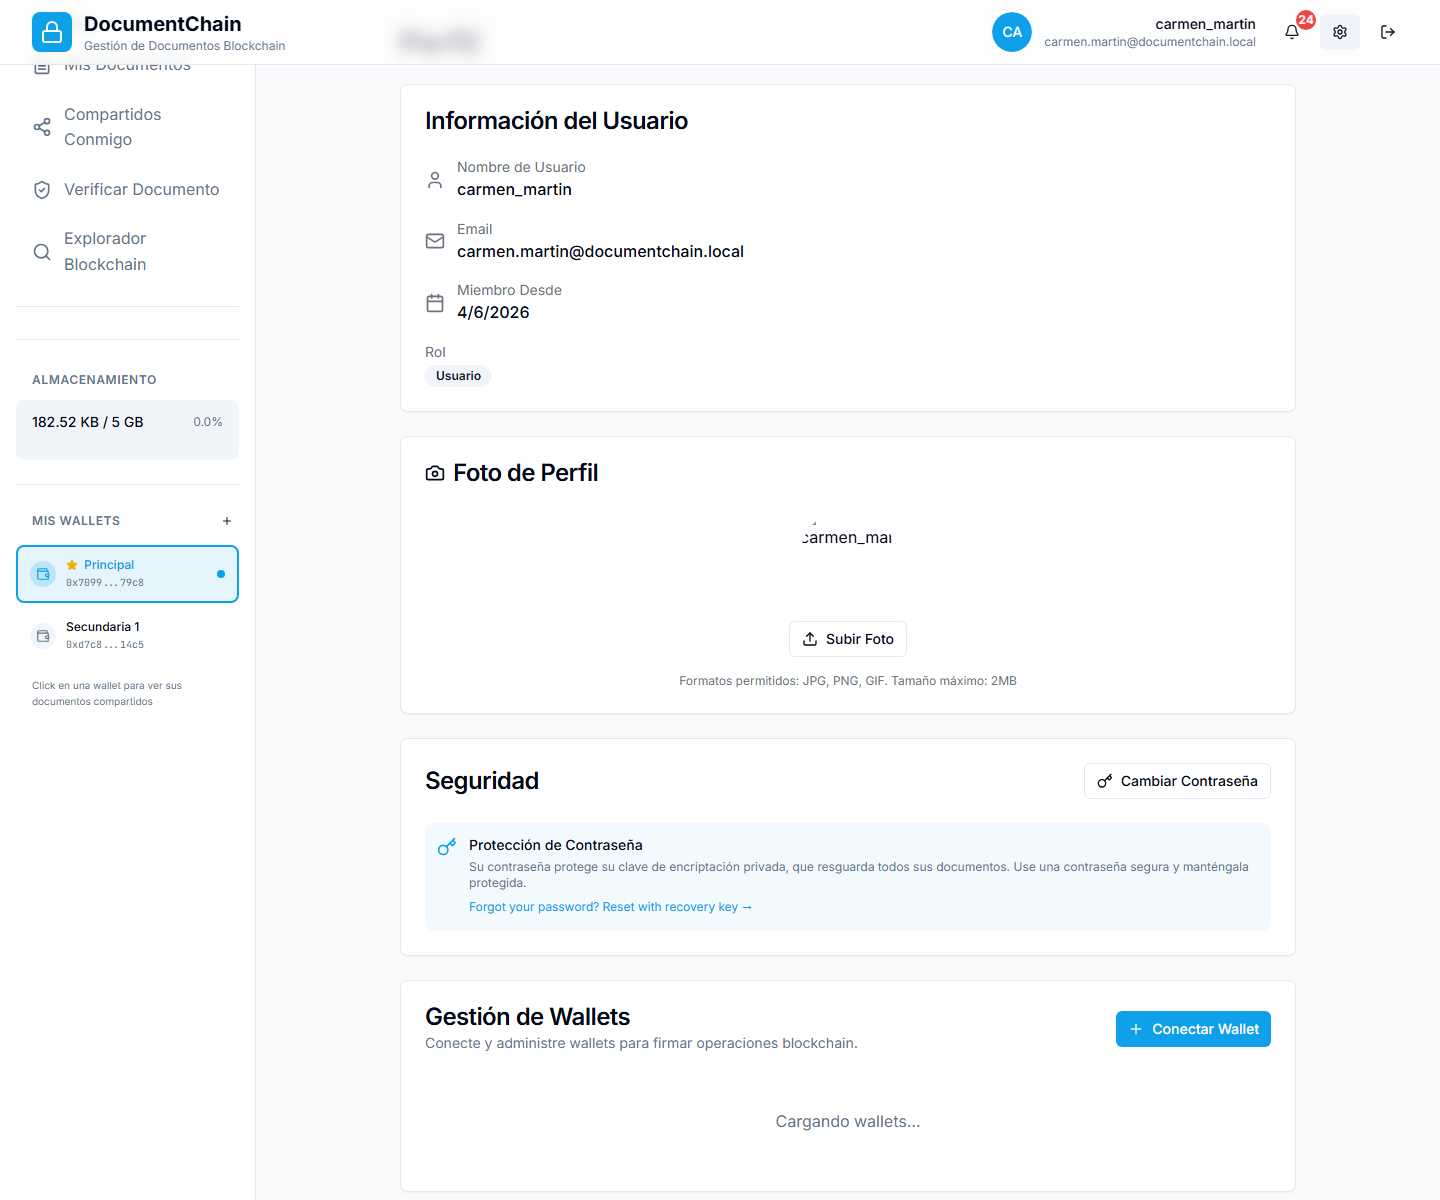
\includegraphics[width=0.9\textwidth]{capturas-ui/profile-page.png}
    \caption{Perfil de usuario y gestión de wallets}
    \label{fig:profile}
\end{figure}

\textbf{Elementos}:
\begin{itemize}
    \item Información personal básica del usuario autenticado.
    \item Gestión de wallets guardadas: alta, etiquetado, selección de principal y eliminación.
    \item Cambio de contraseña dentro del propio perfil.
    \item Soporte para el flujo posterior al registro cuando se desea enlazar wallet inmediatamente.
\end{itemize}

\subsubsection{Vista de configuración}

\begin{figure}[H]
    \centering
    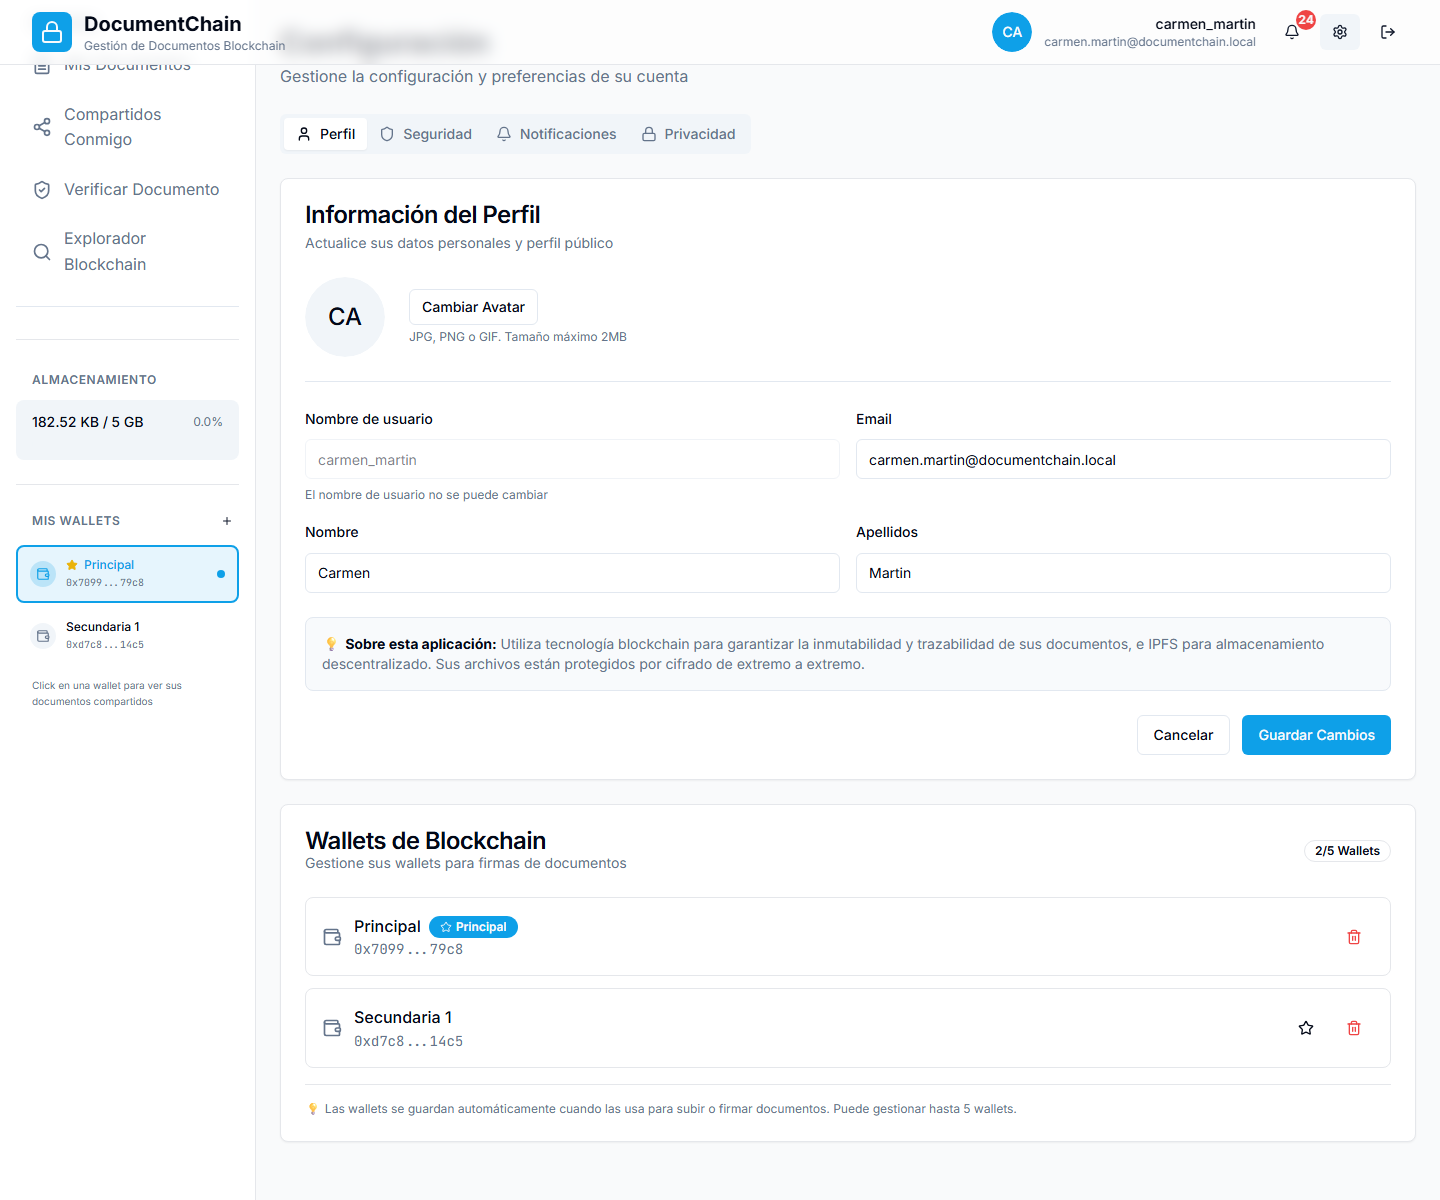
\includegraphics[width=0.9\textwidth]{capturas-ui/settings-page.png}
    \caption{Configuración del usuario}
    \label{fig:settings-ui}
\end{figure}

\textbf{Elementos}:
\begin{itemize}
    \item Pestañas de perfil, seguridad, notificaciones y privacidad.
    \item Configuración de 2FA, regeneración de códigos de respaldo y cambio de contraseña.
    \item Preferencias de notificaciones y opciones de privacidad de cuenta.
    \item Exportación de datos y suspensión/reactivación voluntaria de la cuenta.
\end{itemize}

\subsubsection{Vista de notificaciones}

\begin{figure}[H]
    \centering
    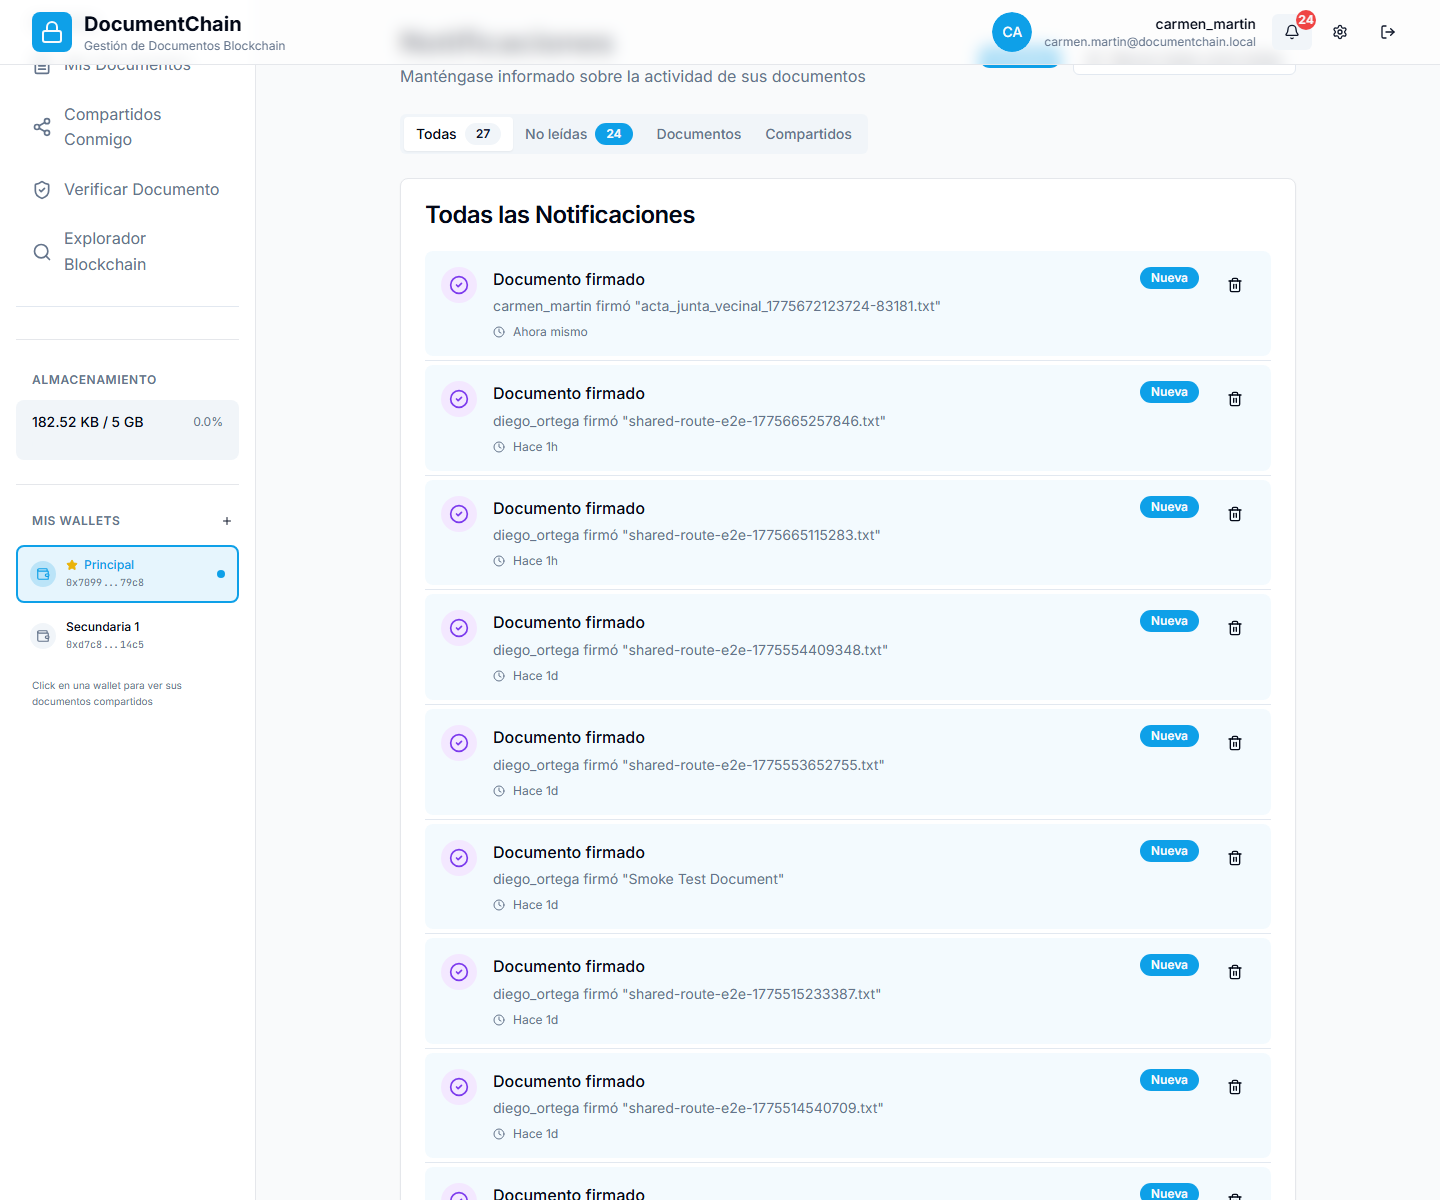
\includegraphics[width=0.9\textwidth]{capturas-ui/notifications-page.png}
    \caption{Panel de notificaciones}
    \label{fig:notifications}
\end{figure}

\textbf{Elementos}:
\begin{itemize}
    \item Listado de notificaciones agrupables por pestañas funcionales.
    \item Acceso contextual al documento u operación relacionada.
    \item Gestión de lectura y borrado de entradas individuales.
    \item Cobertura de eventos de compartición, firma y actividad documental relevante.
\end{itemize}

\section{Diseño procedimental}

\subsection{Diagramas de secuencia}

Los diagramas de secuencia muestran la interacción entre actores y componentes para casos de uso importantes.

\textbf{NOTA}: Los diagramas se generan con PlantUML usando estereotipos boundary, control, entity para representar capas arquitectúnicas.

\subsubsection{Secuencia: Registro de usuario}

\begin{figure}[H]
    \centering
    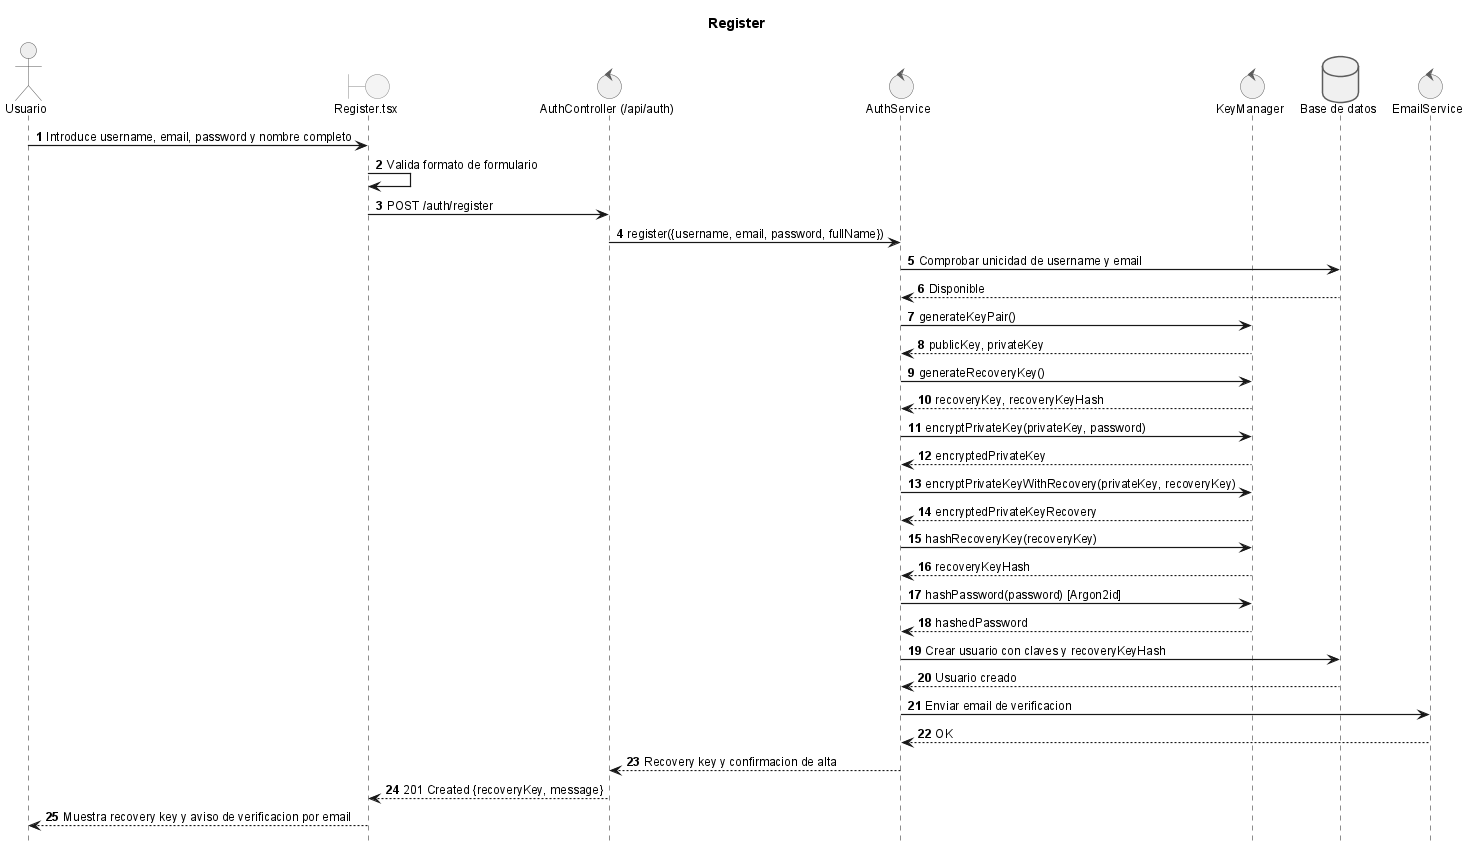
\includegraphics[width=0.9\textwidth]{diagramas/seq-register.png}
    \caption{Diagrama de secuencia UC-0001: Registrar Usuario}
    \label{fig:seq-register}
\end{figure}

\subsubsection{Secuencia: Registro con contraseña y enlace posterior de wallet}

En la versión final del sistema, el registro se realiza exclusivamente con credenciales tradicionales. La vinculación de wallet se desacopla del alta inicial y se ejecuta después de que el usuario ya dispone de sesión válida. Por ese motivo, el flujo de enlace queda representado en la secuencia \ref{fig:seq-connect-wallet}, mientras que el alta base se mantiene en la Figura \ref{fig:seq-register}.

\begin{figure}[H]
    \centering
    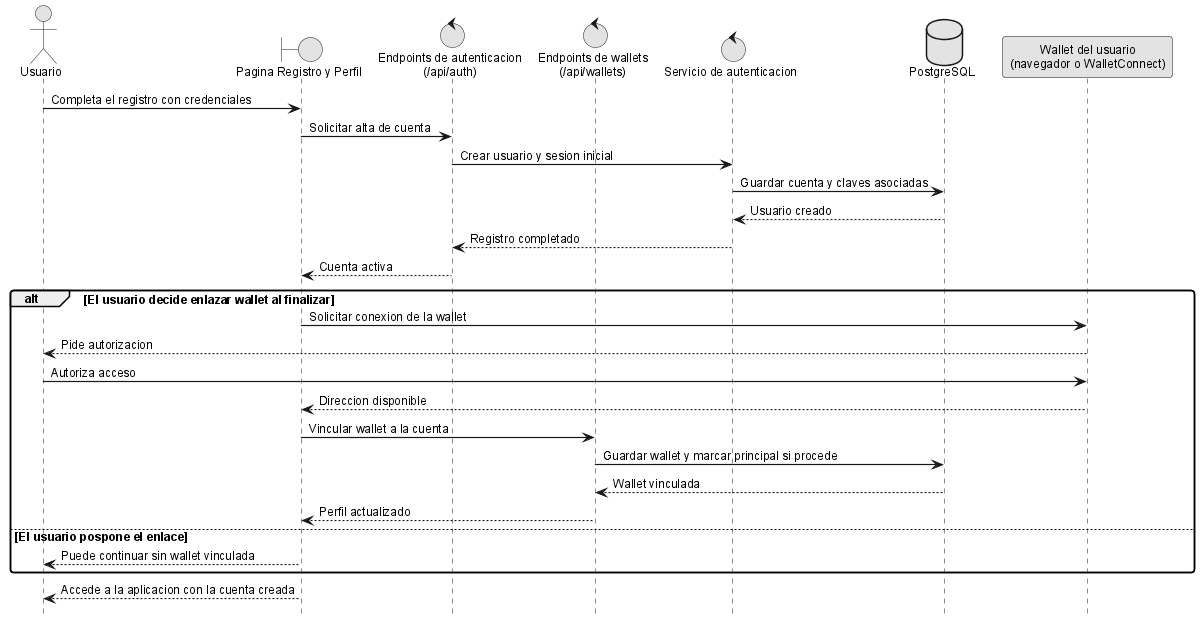
\includegraphics[width=0.9\textwidth]{diagramas/seq-register-wallet.png}
    \caption{Diagrama de secuencia UC-0002: Registrar Usuario y Vincular Wallet Opcionalmente}
    \label{fig:seq-register-wallet}
\end{figure}

\subsubsection{Secuencia: Iniciar Sesión}

\begin{figure}[H]
    \centering
    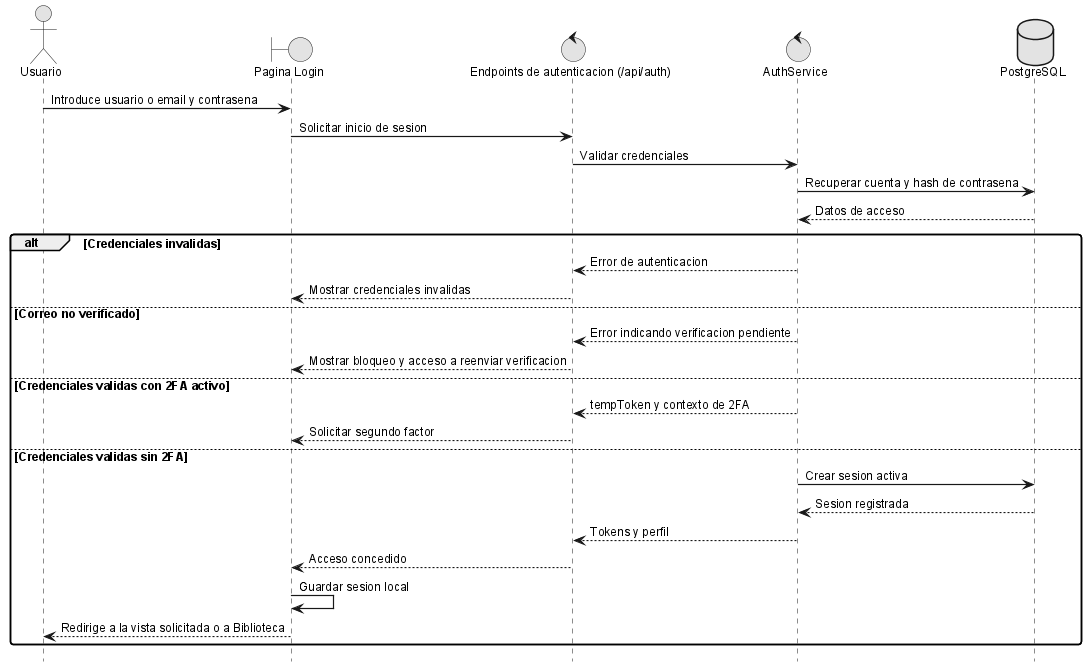
\includegraphics[width=0.9\textwidth]{diagramas/seq-login.png}
    \caption{Diagrama de secuencia UC-0003: Iniciar Sesión}
    \label{fig:seq-login}
\end{figure}

\subsubsection{Secuencia: Verificación 2FA durante el inicio de sesión}

\begin{figure}[H]
    \centering
    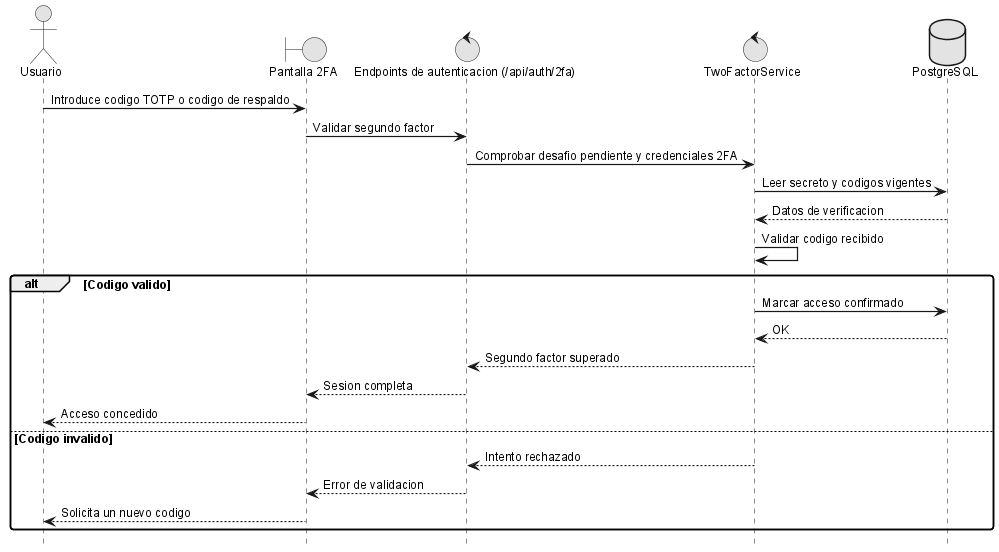
\includegraphics[width=0.9\textwidth]{diagramas/seq-2fa.png}
    \caption{Diagrama de secuencia UC-0004: Validar Segundo Factor en el Inicio de Sesión}
    \label{fig:seq-login-2fa}
\end{figure}

\subsubsection{Secuencia: Cerrar Sesión}

\begin{figure}[H]
    \centering
    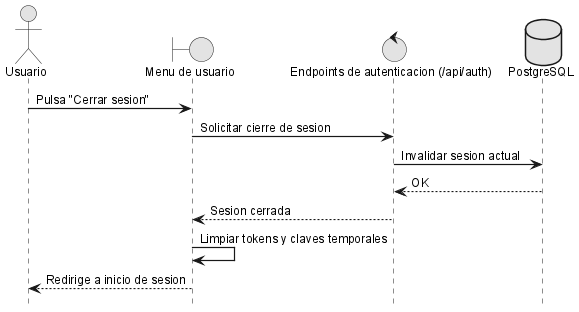
\includegraphics[width=0.9\textwidth]{diagramas/seq-logout.png}
    \caption{Diagrama de secuencia UC-0005: Cerrar Sesión}
    \label{fig:seq-logout}
\end{figure}

\subsubsection{Secuencia: Conectar Wallet}

\begin{figure}[H]
    \centering
    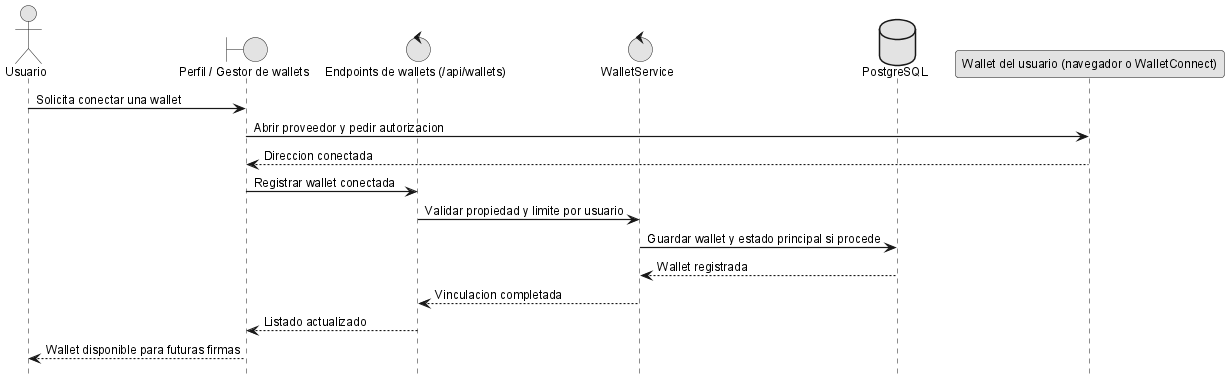
\includegraphics[width=0.9\textwidth]{diagramas/seq-connect-wallet.png}
    \caption{Diagrama de secuencia UC-0006: Conectar Wallet}
    \label{fig:seq-connect-wallet}
\end{figure}
%
% === fin PlantUML ===

\begin{figure}[H]
    \centering
    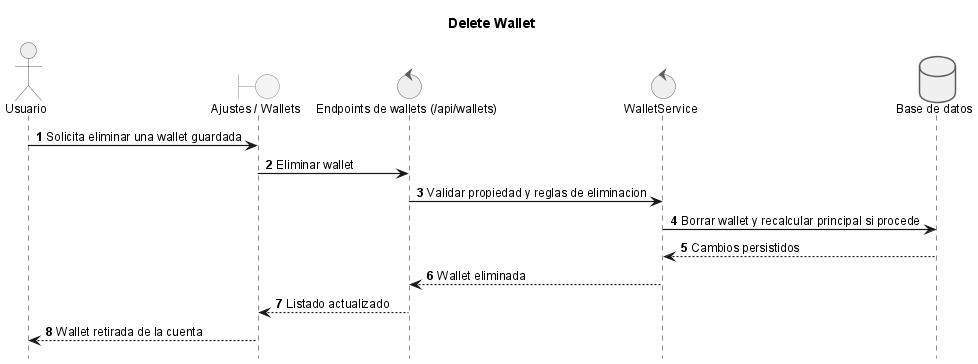
\includegraphics[width=0.9\textwidth]{diagramas/seq-delete-wallet.png}
    \caption{Diagrama de secuencia UC-0007: Eliminar Wallet}
    \label{fig:seq-delete-wallet}
\end{figure}
%
% === fin PlantUML ===

\begin{figure}[H]
    \centering
    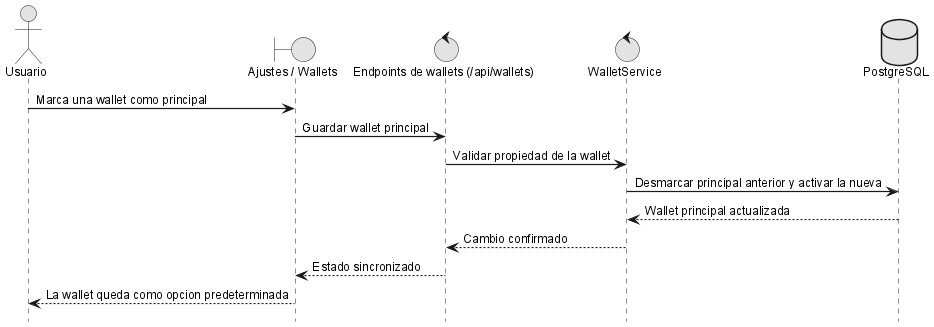
\includegraphics[width=0.9\textwidth]{diagramas/seq-primary-wallet.png}
    \caption{Diagrama de secuencia UC-0008: Establecer Wallet Principal}
    \label{fig:seq-primary-wallet}
\end{figure}
%
% === fin PlantUML ===

\begin{figure}[H]
    \centering
    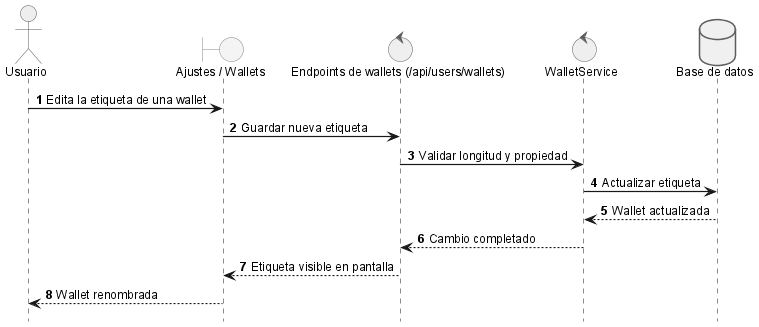
\includegraphics[width=0.9\textwidth]{diagramas/seq-label-wallet.png}
    \caption{Diagrama de secuencia UC-0009: Renombrar/Etiquetar Wallet}
    \label{fig:seq-label-wallet}
\end{figure}

\subsubsection{Secuencia: Gestionar Perfil}

\begin{figure}[H]
    \centering
    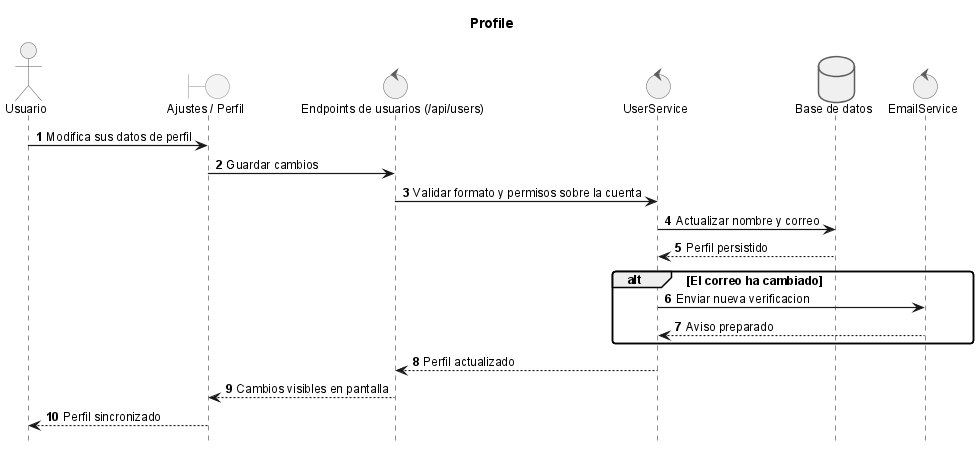
\includegraphics[width=0.9\textwidth]{diagramas/seq-profile.png}
    \caption{Diagrama de secuencia UC-0010: Gestionar Perfil}
    \label{fig:seq-profile}
\end{figure}
%
% === fin PlantUML ===

\begin{figure}[H]
    \centering
    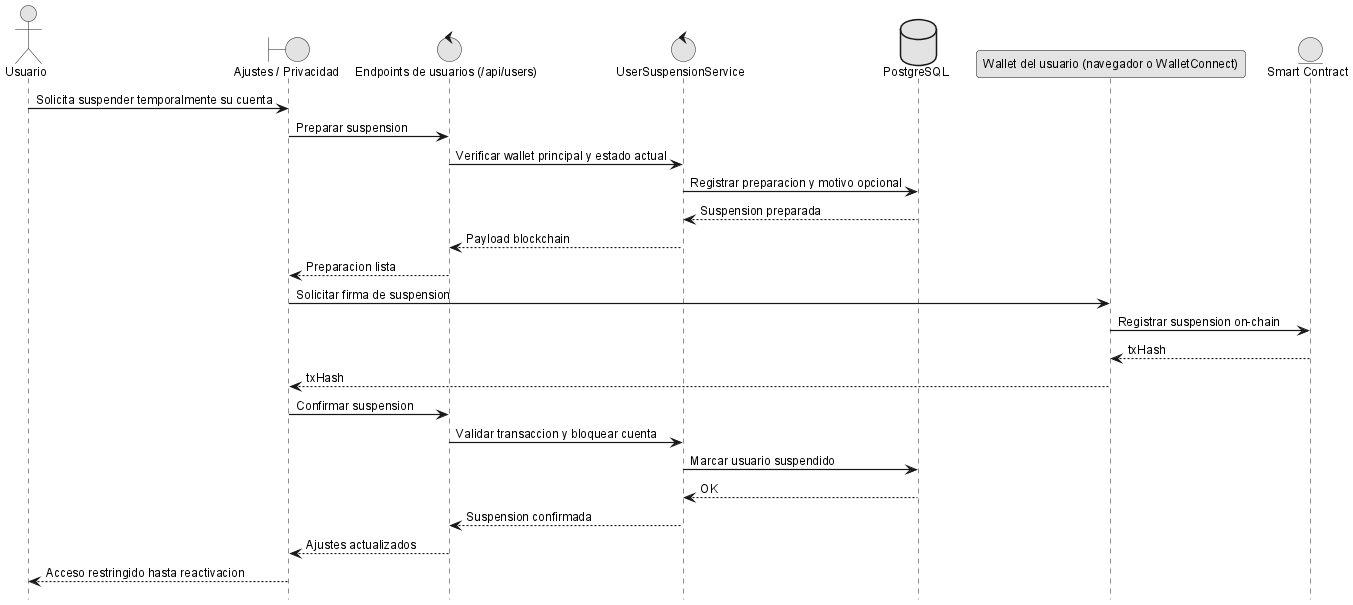
\includegraphics[width=0.9\textwidth]{diagramas/seq-self-suspend.png}
    \caption{Diagrama de secuencia UC-0011: Desactivar Propia Cuenta}
    \label{fig:seq-self-suspend}
\end{figure}
%
% === fin PlantUML ===

\begin{figure}[H]
    \centering
    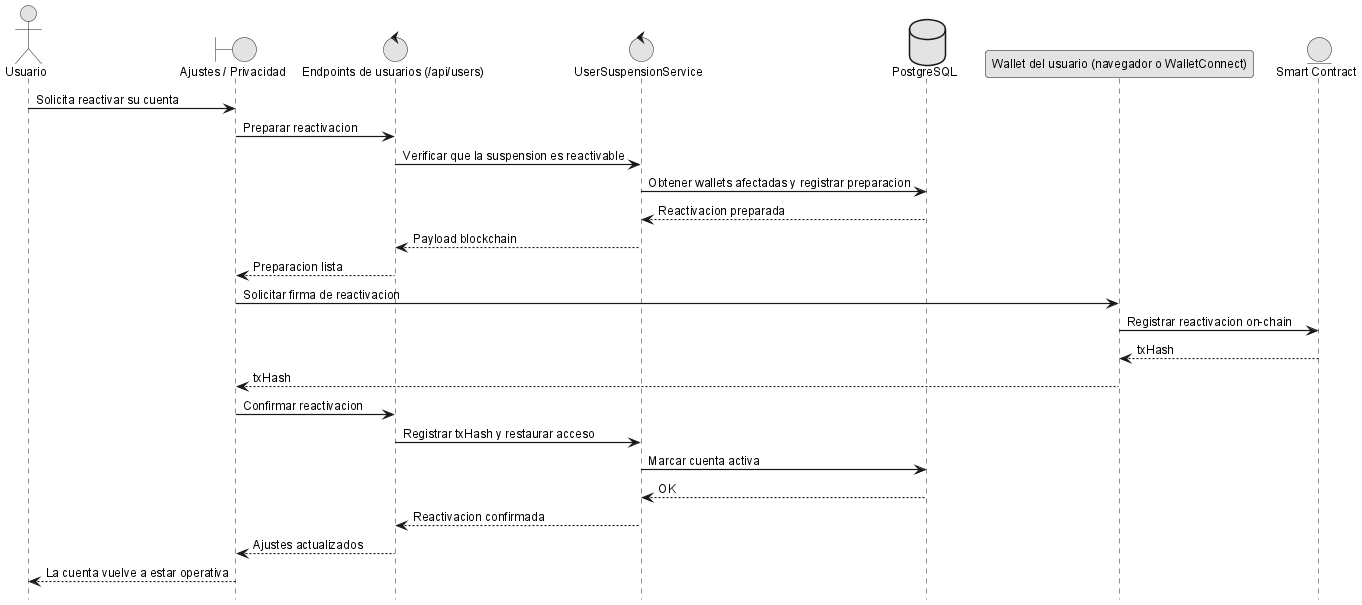
\includegraphics[width=0.9\textwidth]{diagramas/seq-self-unsuspend.png}
    \caption{Diagrama de secuencia UC-0012: Reactivar Propia Cuenta}
    \label{fig:seq-self-unsuspend}
\end{figure}

\subsubsection{Secuencia: Cambiar Contraseña}

\begin{figure}[H]
    \centering
    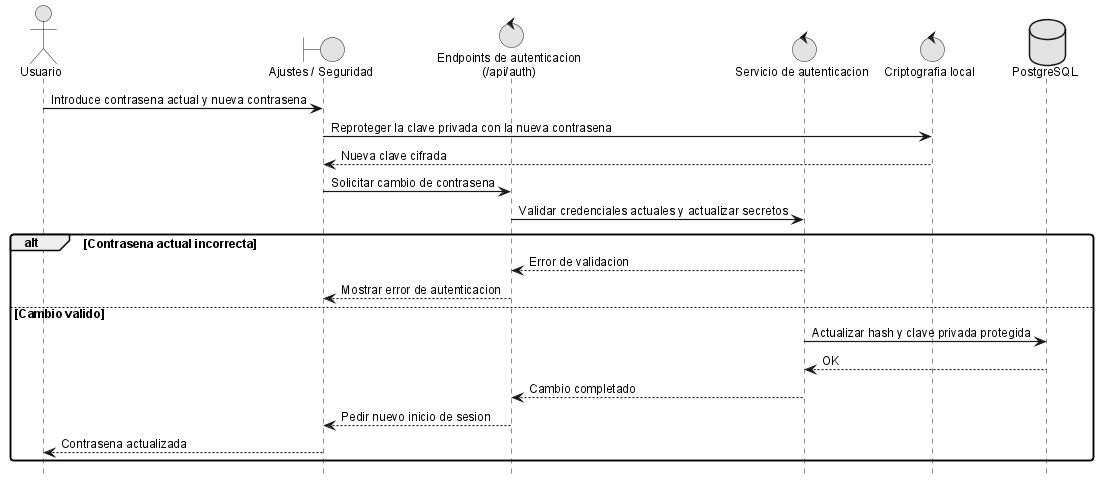
\includegraphics[width=0.9\textwidth]{diagramas/seq-change-password.png}
    \caption{Diagrama de secuencia UC-0013: Cambiar Contraseña}
    \label{fig:seq-change-password}
\end{figure}

\subsubsection{Secuencia: Recuperar Contraseña}

\begin{figure}[H]
    \centering
    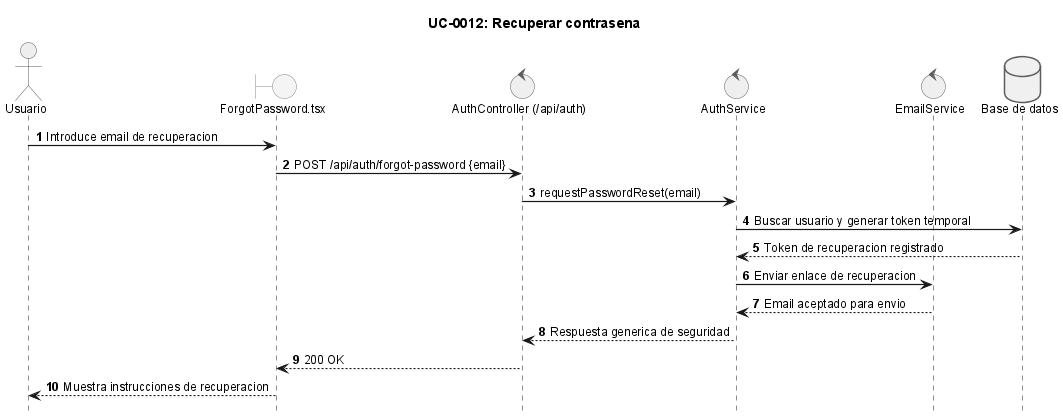
\includegraphics[width=0.9\textwidth]{diagramas/seq-recover-password.png}
    \caption{Diagrama de secuencia UC-0014: Recuperar Contraseña}
    \label{fig:seq-recover-password}
\end{figure}

\subsubsection{Secuencia: Verificar Email}

\begin{figure}[H]
    \centering
    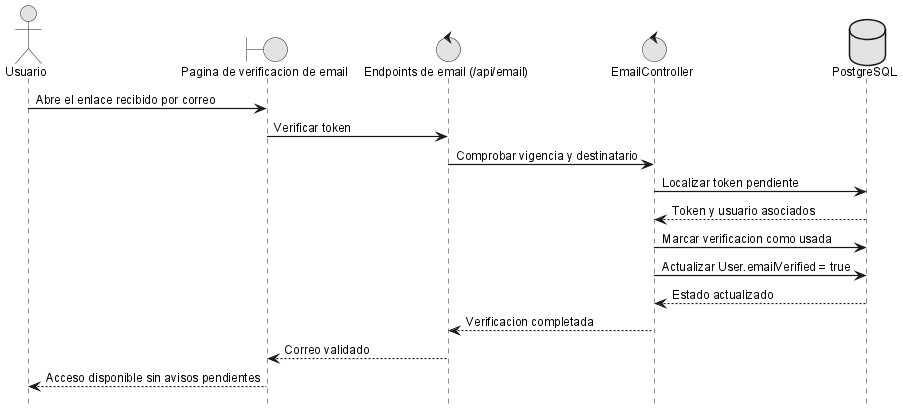
\includegraphics[width=0.9\textwidth]{diagramas/seq-verify-email.png}
    \caption{Diagrama de secuencia UC-0015: Verificar Email}
    \label{fig:seq-verify-email}
\end{figure}
%
% === fin PlantUML ===

\begin{figure}[H]
    \centering
    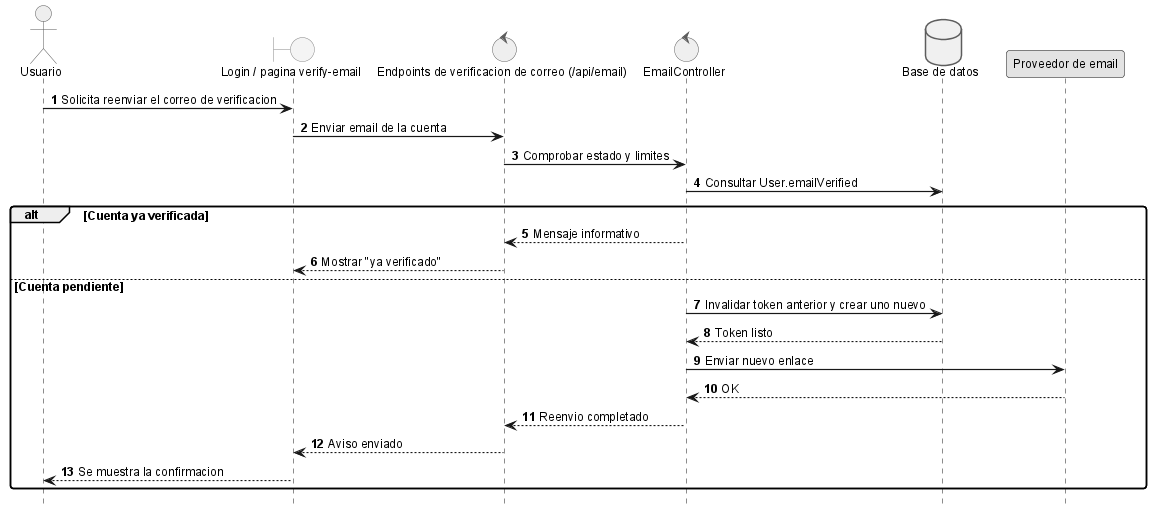
\includegraphics[width=0.9\textwidth]{diagramas/seq-resend-verification.png}
    \caption{Diagrama de secuencia UC-0016: Reenviar Email de Verificación}
    \label{fig:seq-resend-verification}
\end{figure}

\subsubsection{Secuencia: Configurar Autenticación de Dos Factores}

\begin{figure}[H]
    \centering
    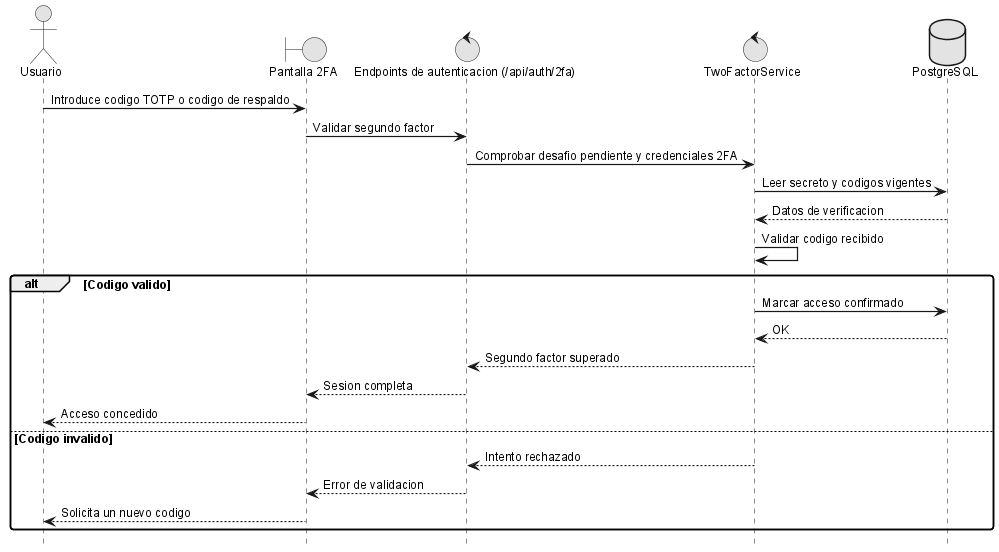
\includegraphics[width=0.9\textwidth]{diagramas/seq-2fa.png}
    \caption{Diagrama de secuencia UC-0017: Configurar 2FA}
    \label{fig:seq-2fa}
\end{figure}
%
% === fin PlantUML ===

\begin{figure}[H]
    \centering
    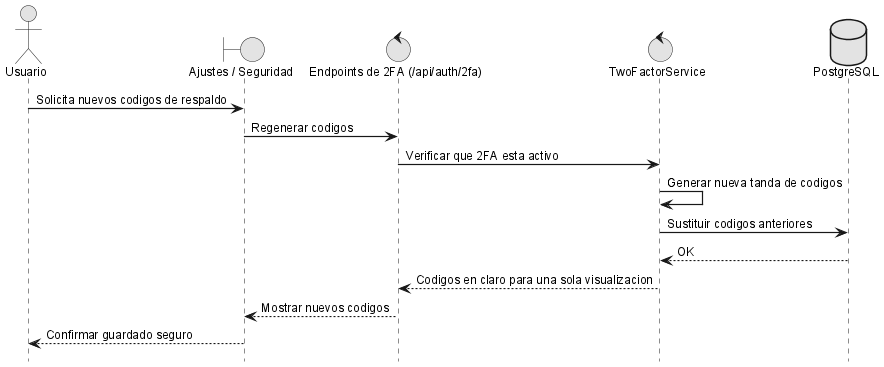
\includegraphics[width=0.9\textwidth]{diagramas/seq-regen-backup-2fa.png}
    \caption{Diagrama de secuencia UC-0018: Regenerar Códigos de Backup 2FA}
    \label{fig:seq-regen-backup-2fa}
\end{figure}

\subsubsection{Secuencia: Subir documento}

\begin{figure}[H]
    \centering
    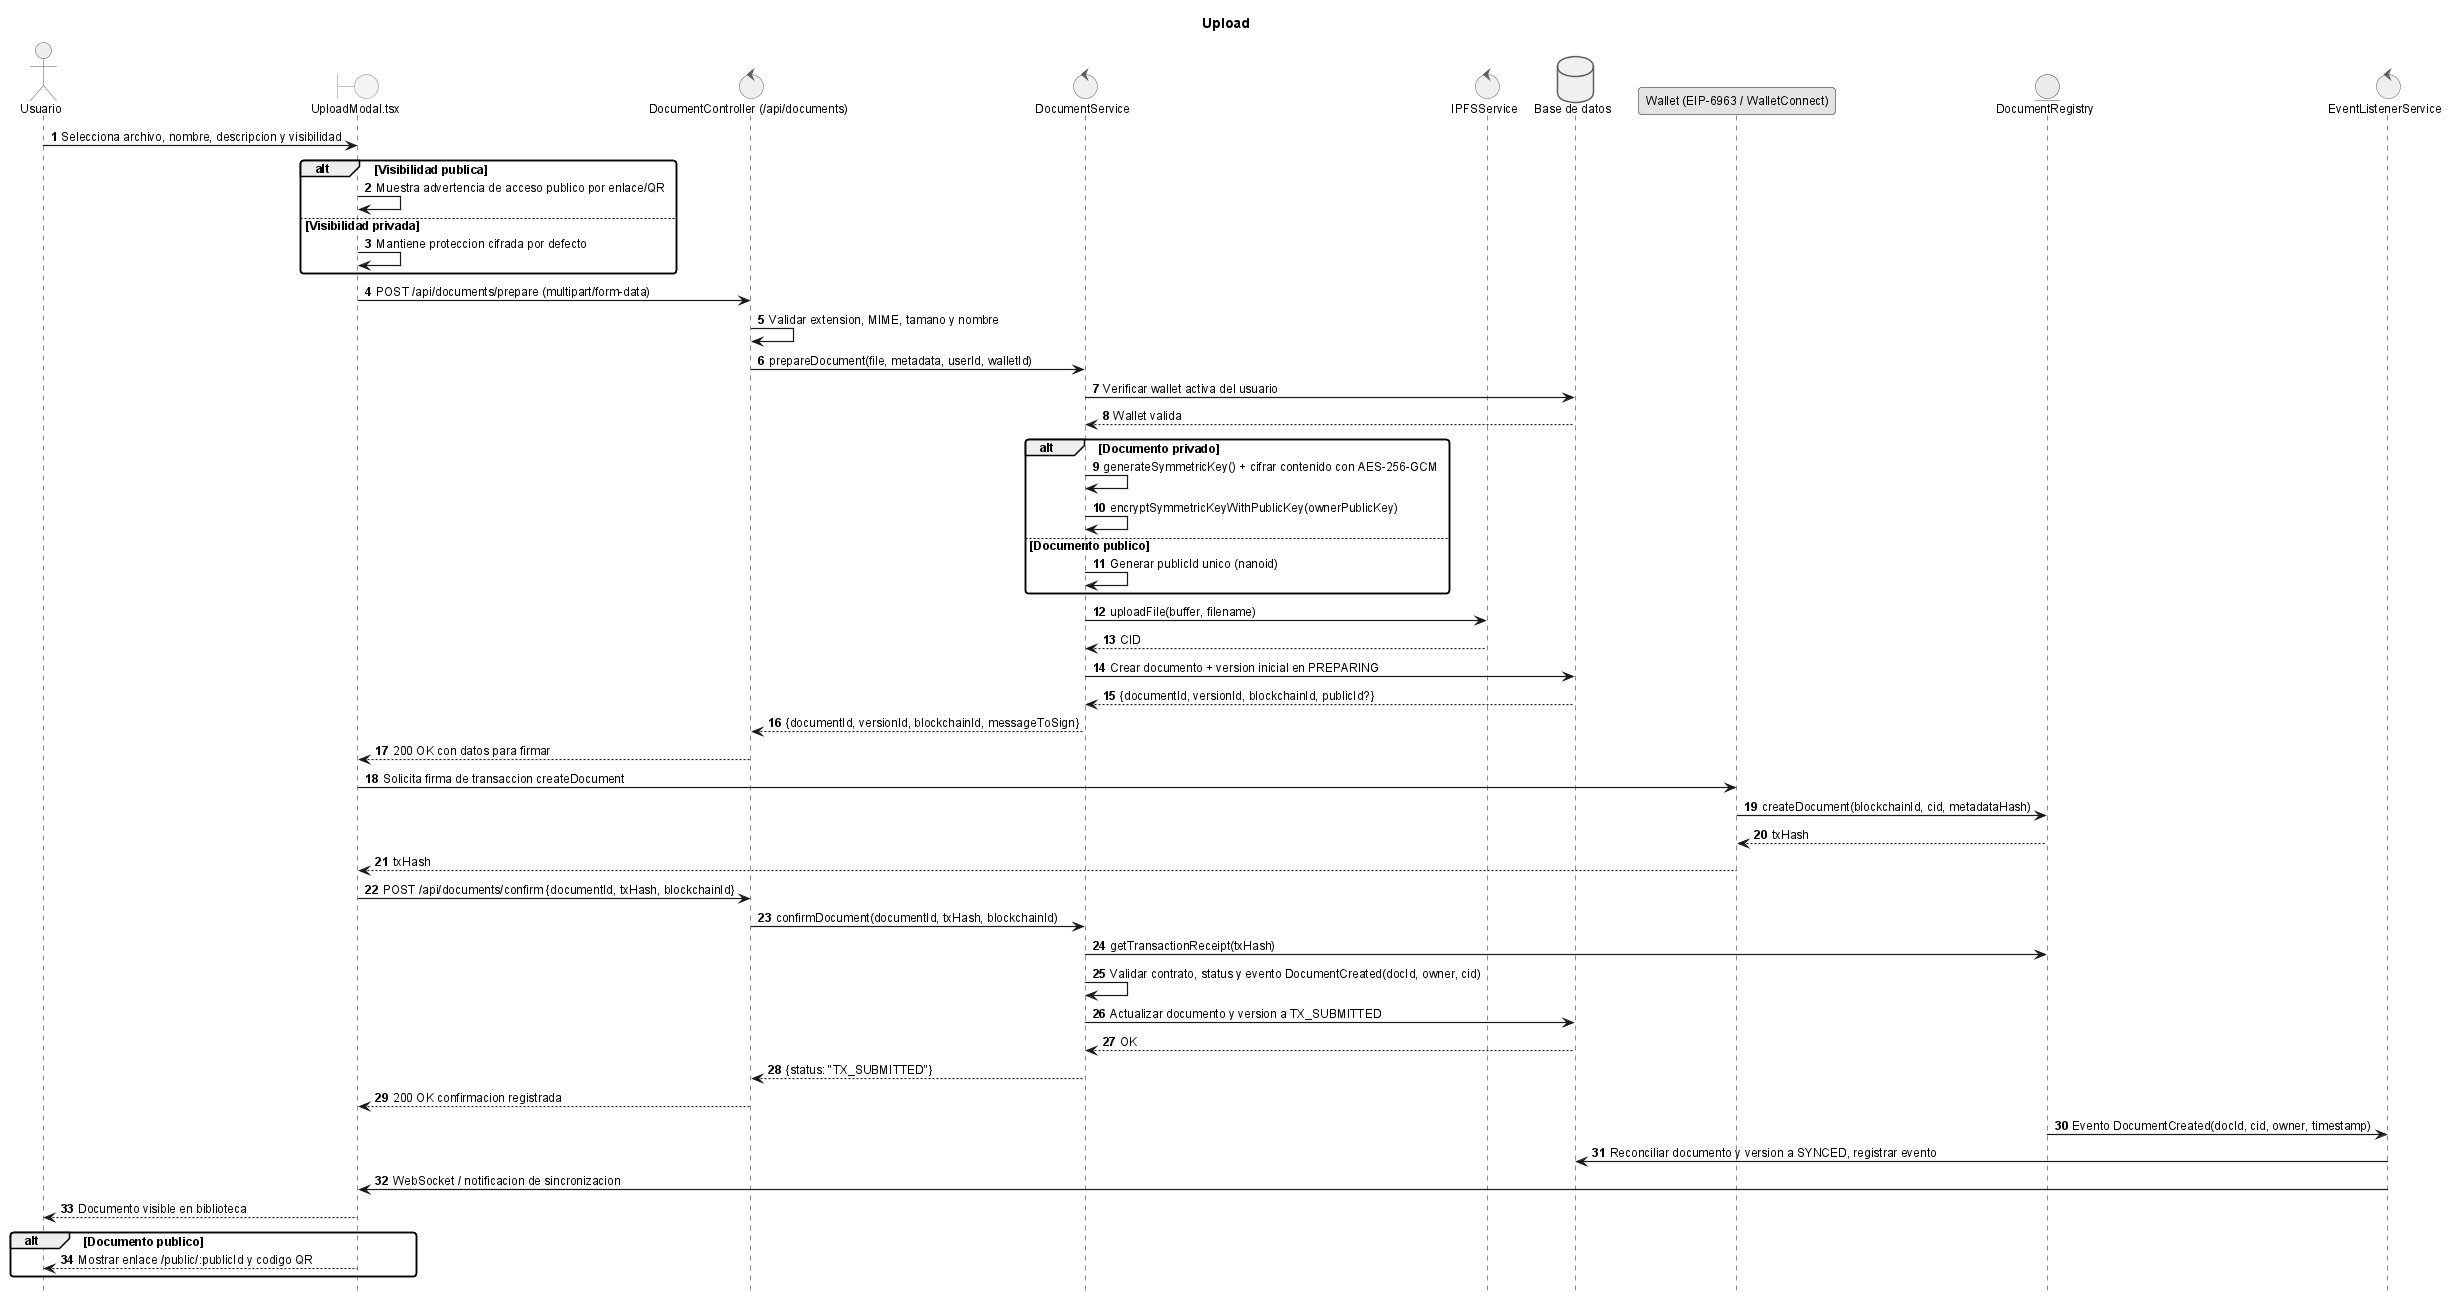
\includegraphics[width=0.9\textwidth]{diagramas/seq-upload.png}
    \caption{Diagrama de secuencia UC-0019: Subir Documento}
    \label{fig:seq-upload}
\end{figure}

\subsubsection{Secuencia: Listar Documentos}

\begin{figure}[H]
    \centering
    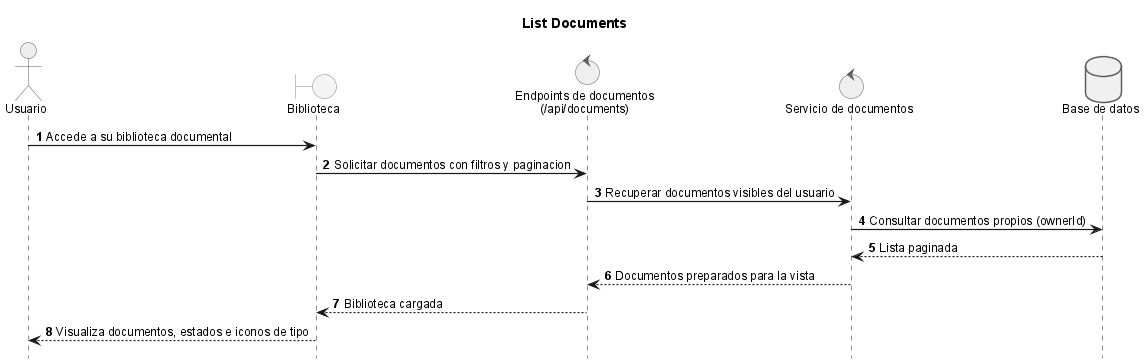
\includegraphics[width=0.9\textwidth]{diagramas/seq-list-documents.png}
    \caption{Diagrama de secuencia UC-0020: Listar Documentos}
    \label{fig:seq-list-documents}
\end{figure}

\subsubsection{Secuencia: Ver Detalle de Documento}

\begin{figure}[H]
    \centering
    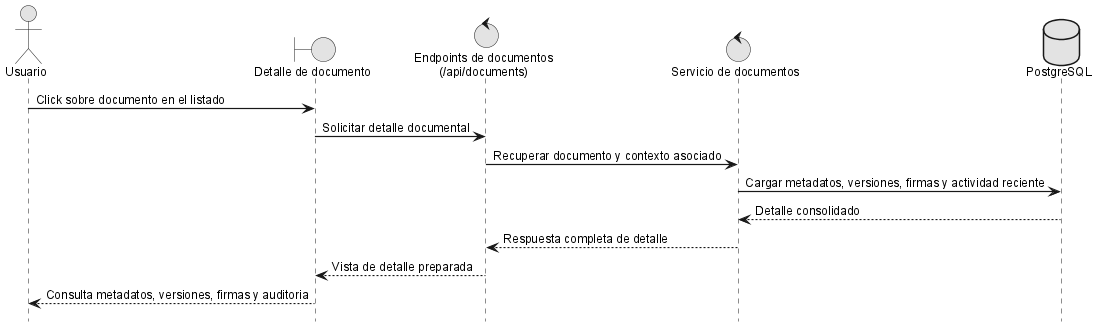
\includegraphics[width=0.9\textwidth]{diagramas/seq-doc-detail.png}
    \caption{Diagrama de secuencia UC-0021: Ver Detalle de Documento}
    \label{fig:seq-doc-detail}
\end{figure}

\subsubsection{Secuencia: Descargar documento}

\begin{figure}[H]
    \centering
    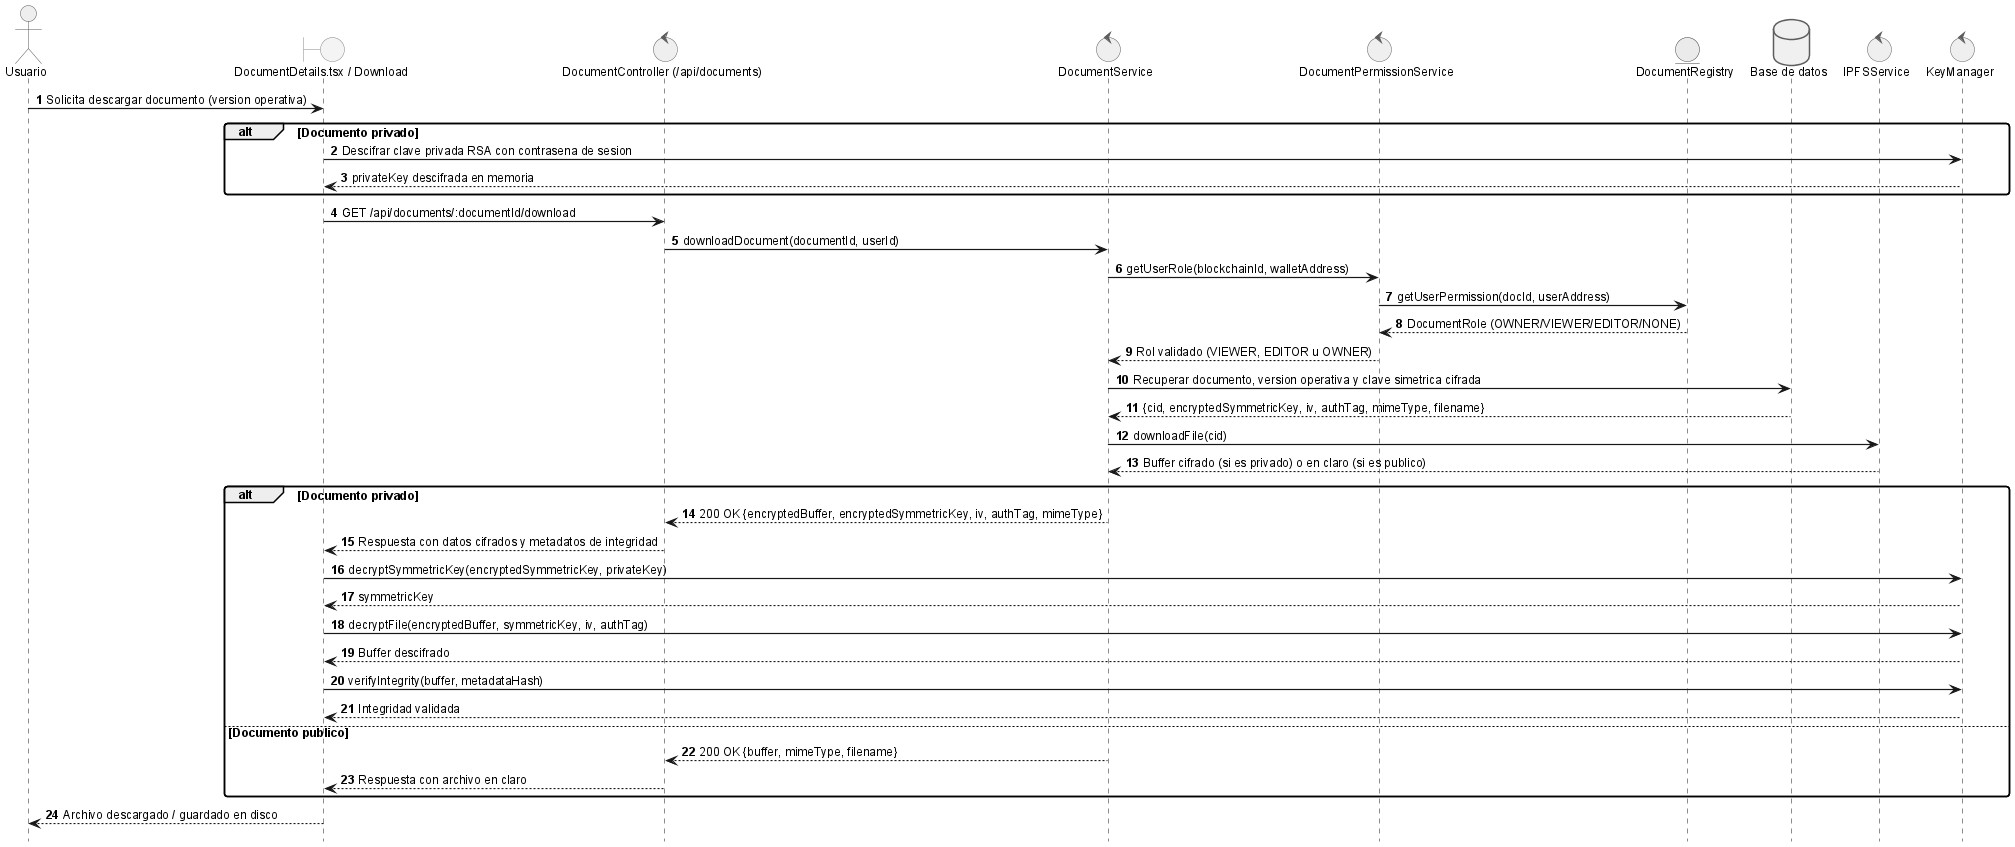
\includegraphics[width=0.9\textwidth]{diagramas/seq-download.png}
    \caption{Diagrama de secuencia UC-0022: Descargar Documento}
    \label{fig:seq-download}
\end{figure}

\subsubsection{Secuencia: Archivar Documento}

\begin{figure}[H]
    \centering
    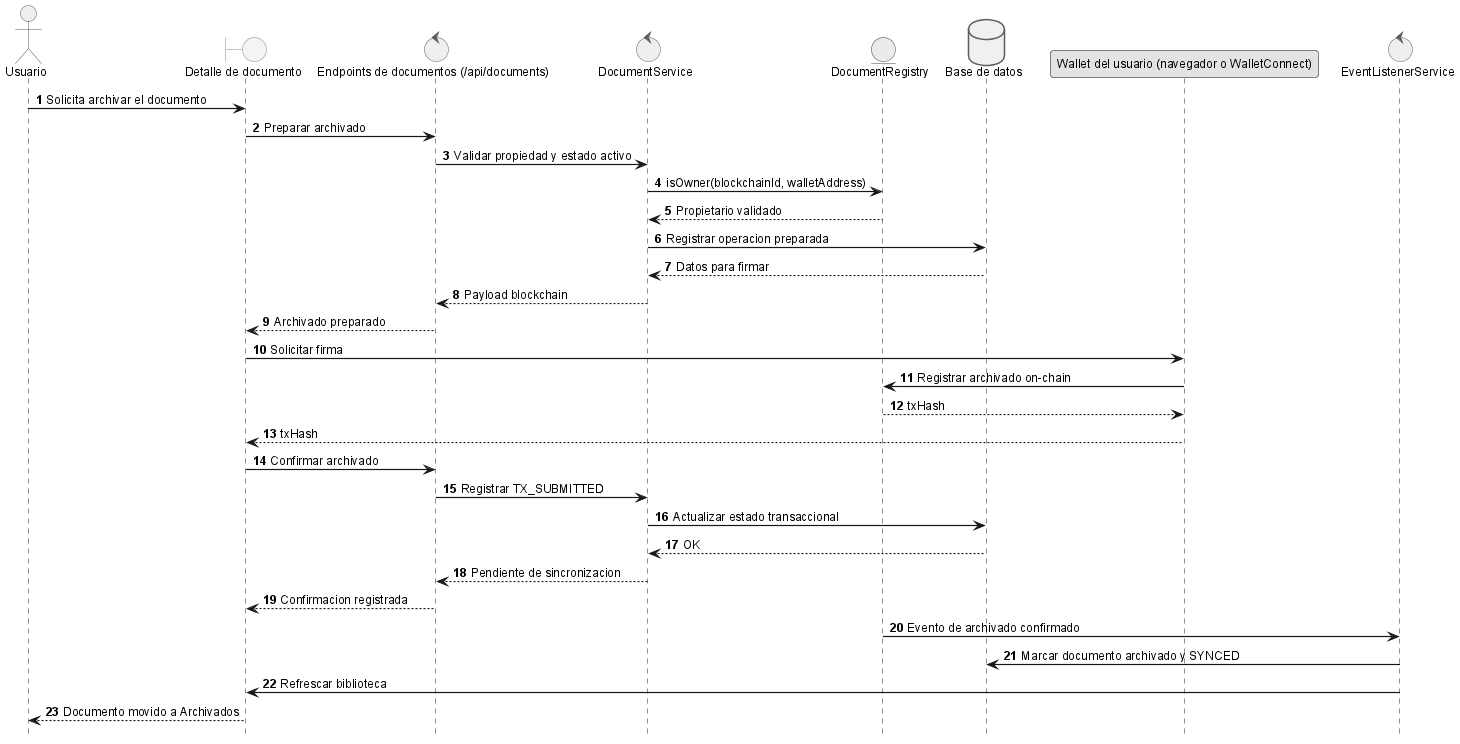
\includegraphics[width=0.9\textwidth]{diagramas/seq-archive.png}
    \caption{Diagrama de secuencia UC-0023: Archivar Documento}
    \label{fig:seq-archive}
\end{figure}
%
% === fin PlantUML ===

\begin{figure}[H]
    \centering
    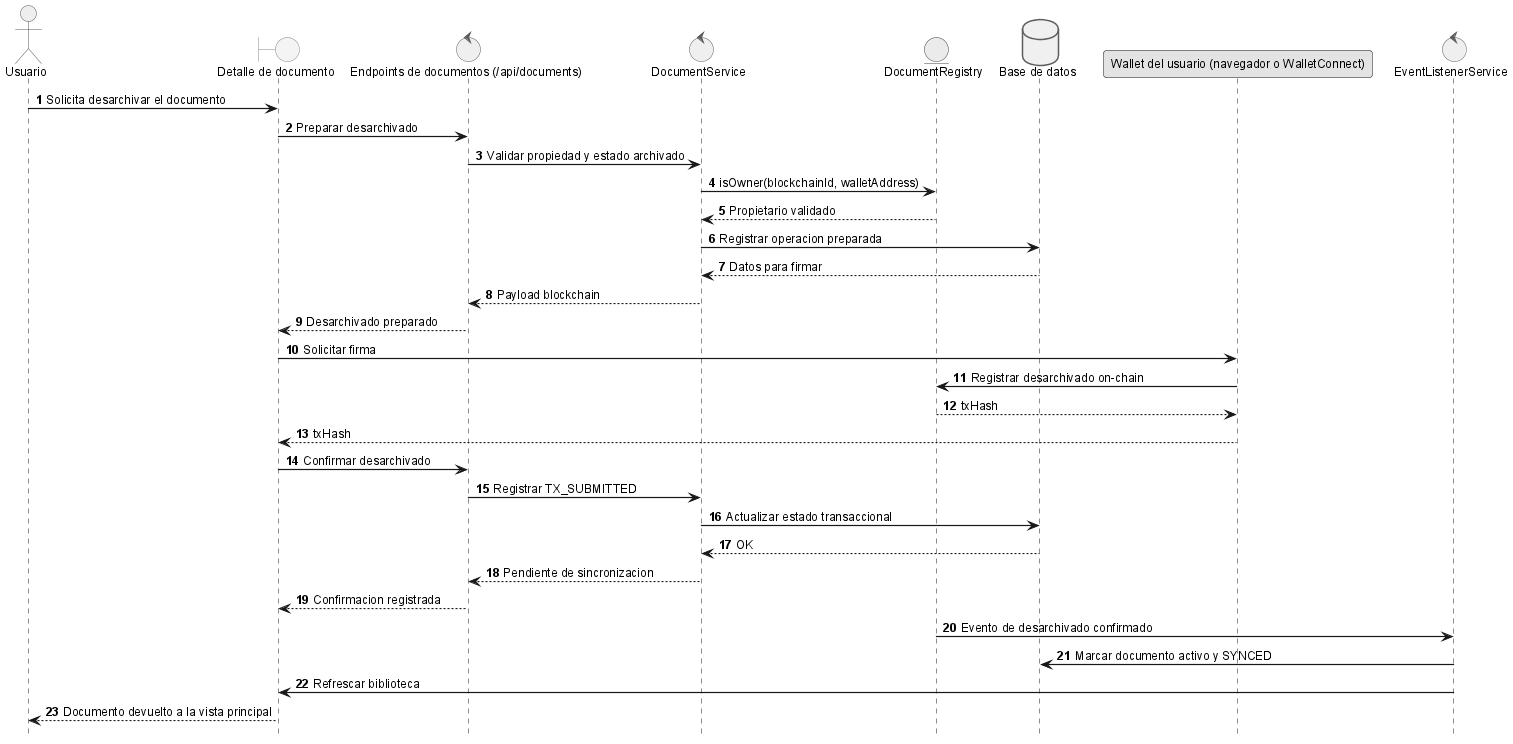
\includegraphics[width=0.9\textwidth]{diagramas/seq-unarchive.png}
    \caption{Diagrama de secuencia UC-0024: Desarchivar Documento}
    \label{fig:seq-unarchive}
\end{figure}

\subsubsection{Secuencia: Eliminar Documento}

\begin{figure}[H]
    \centering
    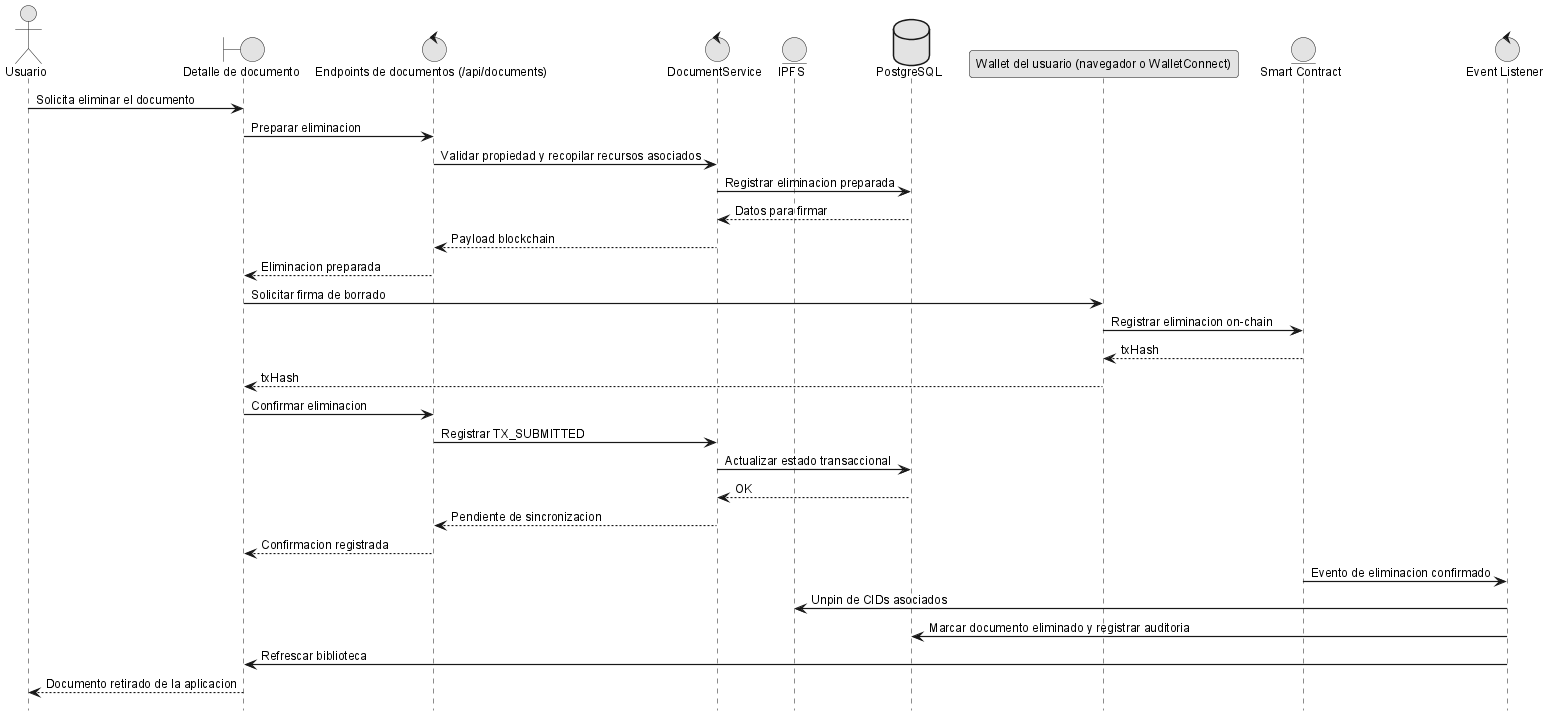
\includegraphics[width=0.9\textwidth]{diagramas/seq-delete.png}
    \caption{Diagrama de secuencia UC-0025: Eliminar Documento}
    \label{fig:seq-delete}
\end{figure}
%
% === fin PlantUML ===

Este flujo se mantiene como referencia de diseño y como soporte de backend, pero no dispone todavía de una interacción específica expuesta en la vista principal de detalle del documento dentro de la entrega actual.

\begin{figure}[H]
    \centering
    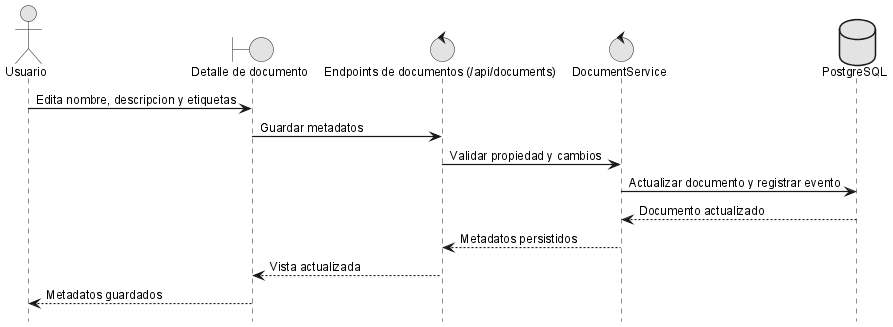
\includegraphics[width=0.9\textwidth]{diagramas/seq-edit-metadata.png}
    \caption{Diagrama de secuencia UC-0026: Editar Metadatos de Documento}
    \label{fig:seq-edit-metadata}
\end{figure}

\subsubsection{Secuencia: Transferir Documento}

\begin{figure}[H]
    \centering
    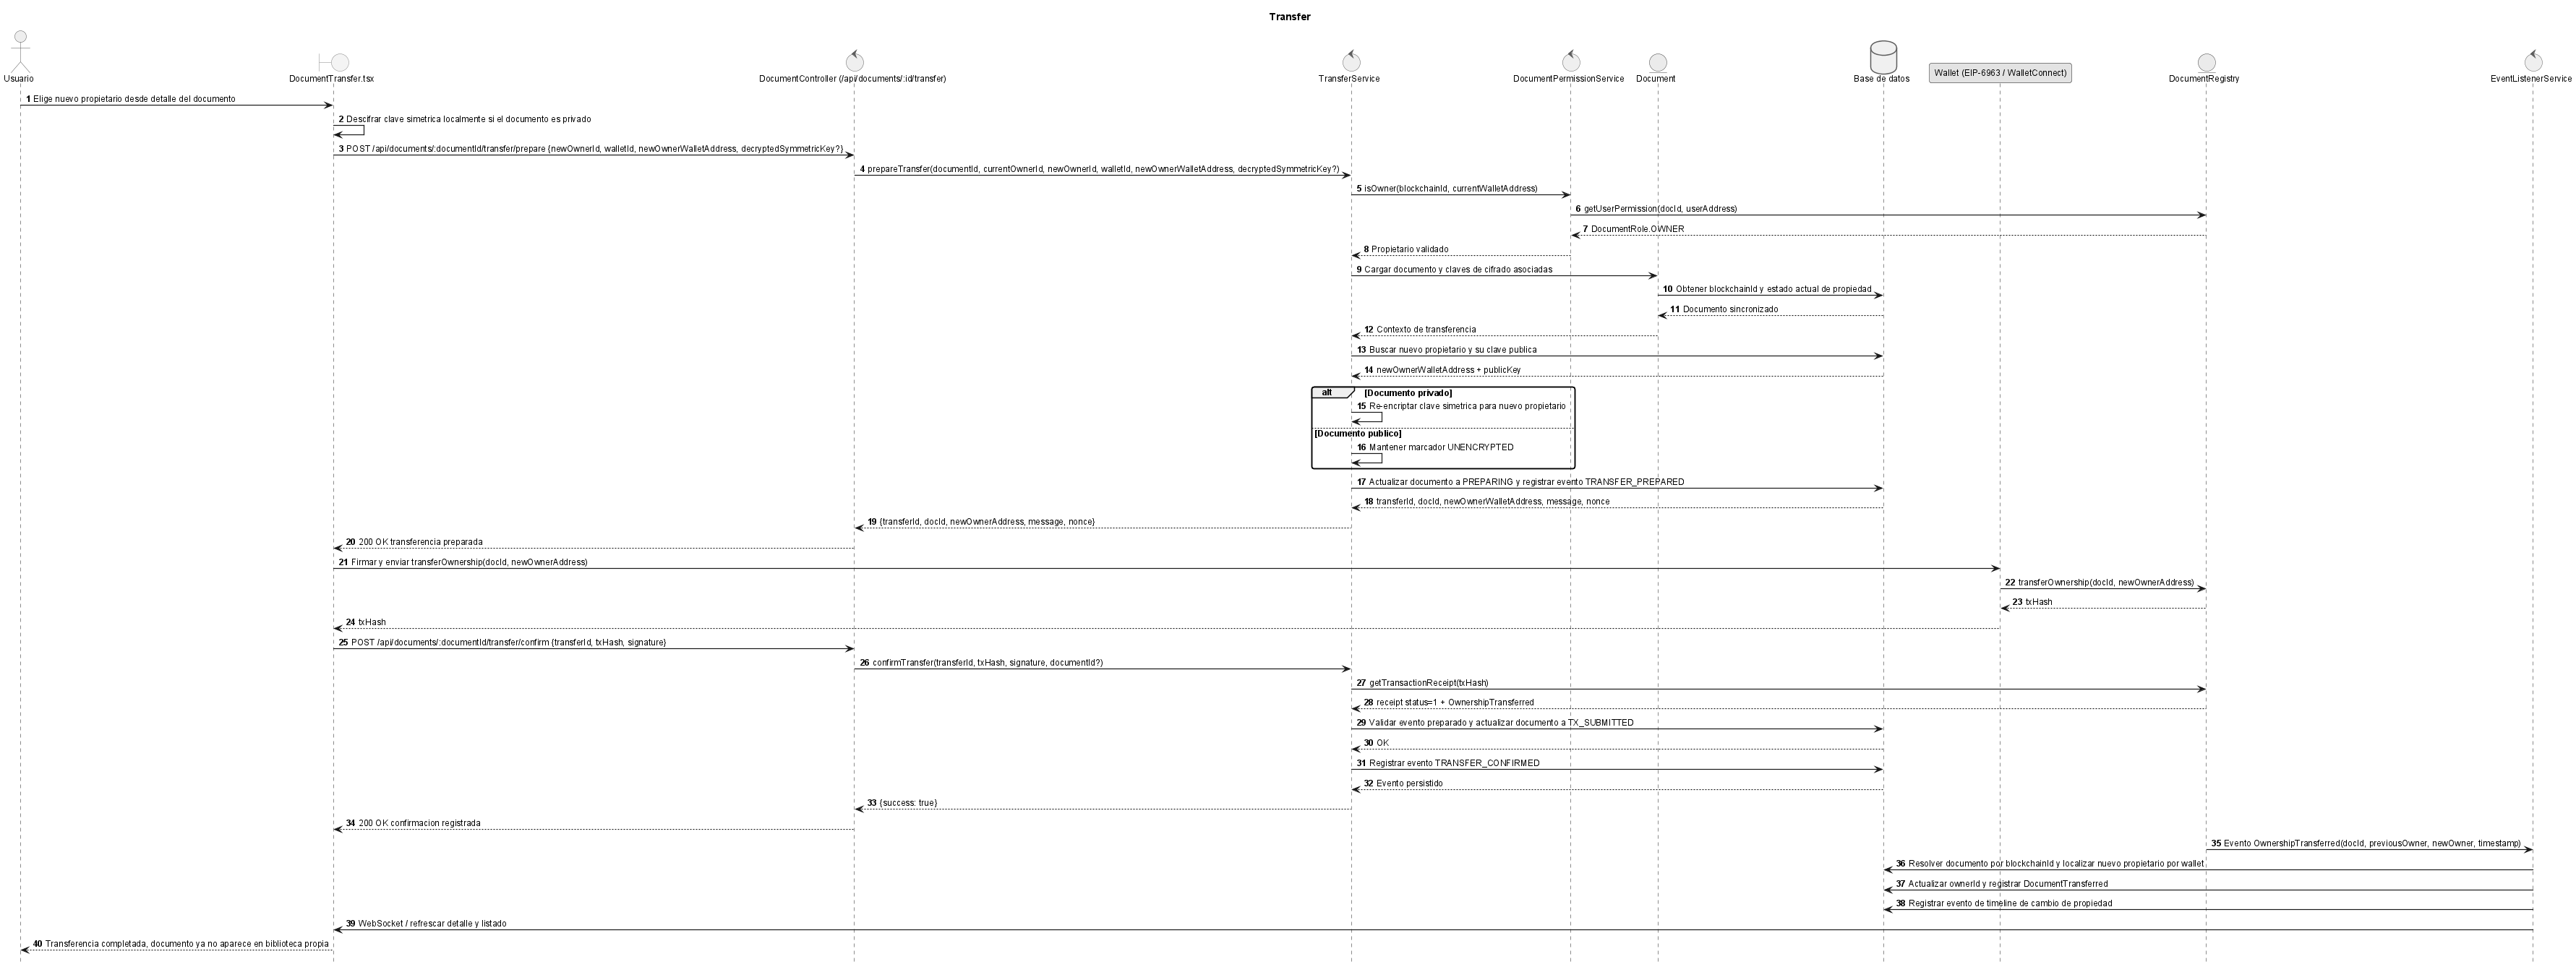
\includegraphics[width=0.9\textwidth]{diagramas/seq-transfer.png}
    \caption{Diagrama de secuencia UC-0027: Transferir Documento}
    \label{fig:seq-transfer}
\end{figure}

\subsubsection{Secuencia: Buscar Documentos}

\begin{figure}[H]
    \centering
    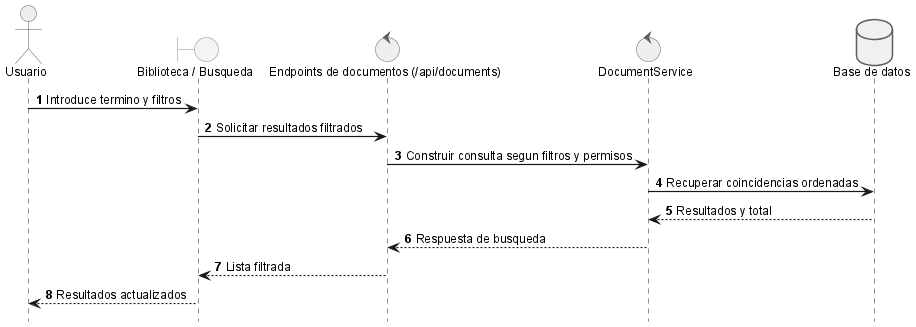
\includegraphics[width=0.9\textwidth]{diagramas/seq-search.png}
    \caption{Diagrama de secuencia UC-0028: Buscar Documentos}
    \label{fig:seq-search}
\end{figure}

\subsubsection{Secuencia: Crear nueva versión}

\begin{figure}[H]
    \centering
    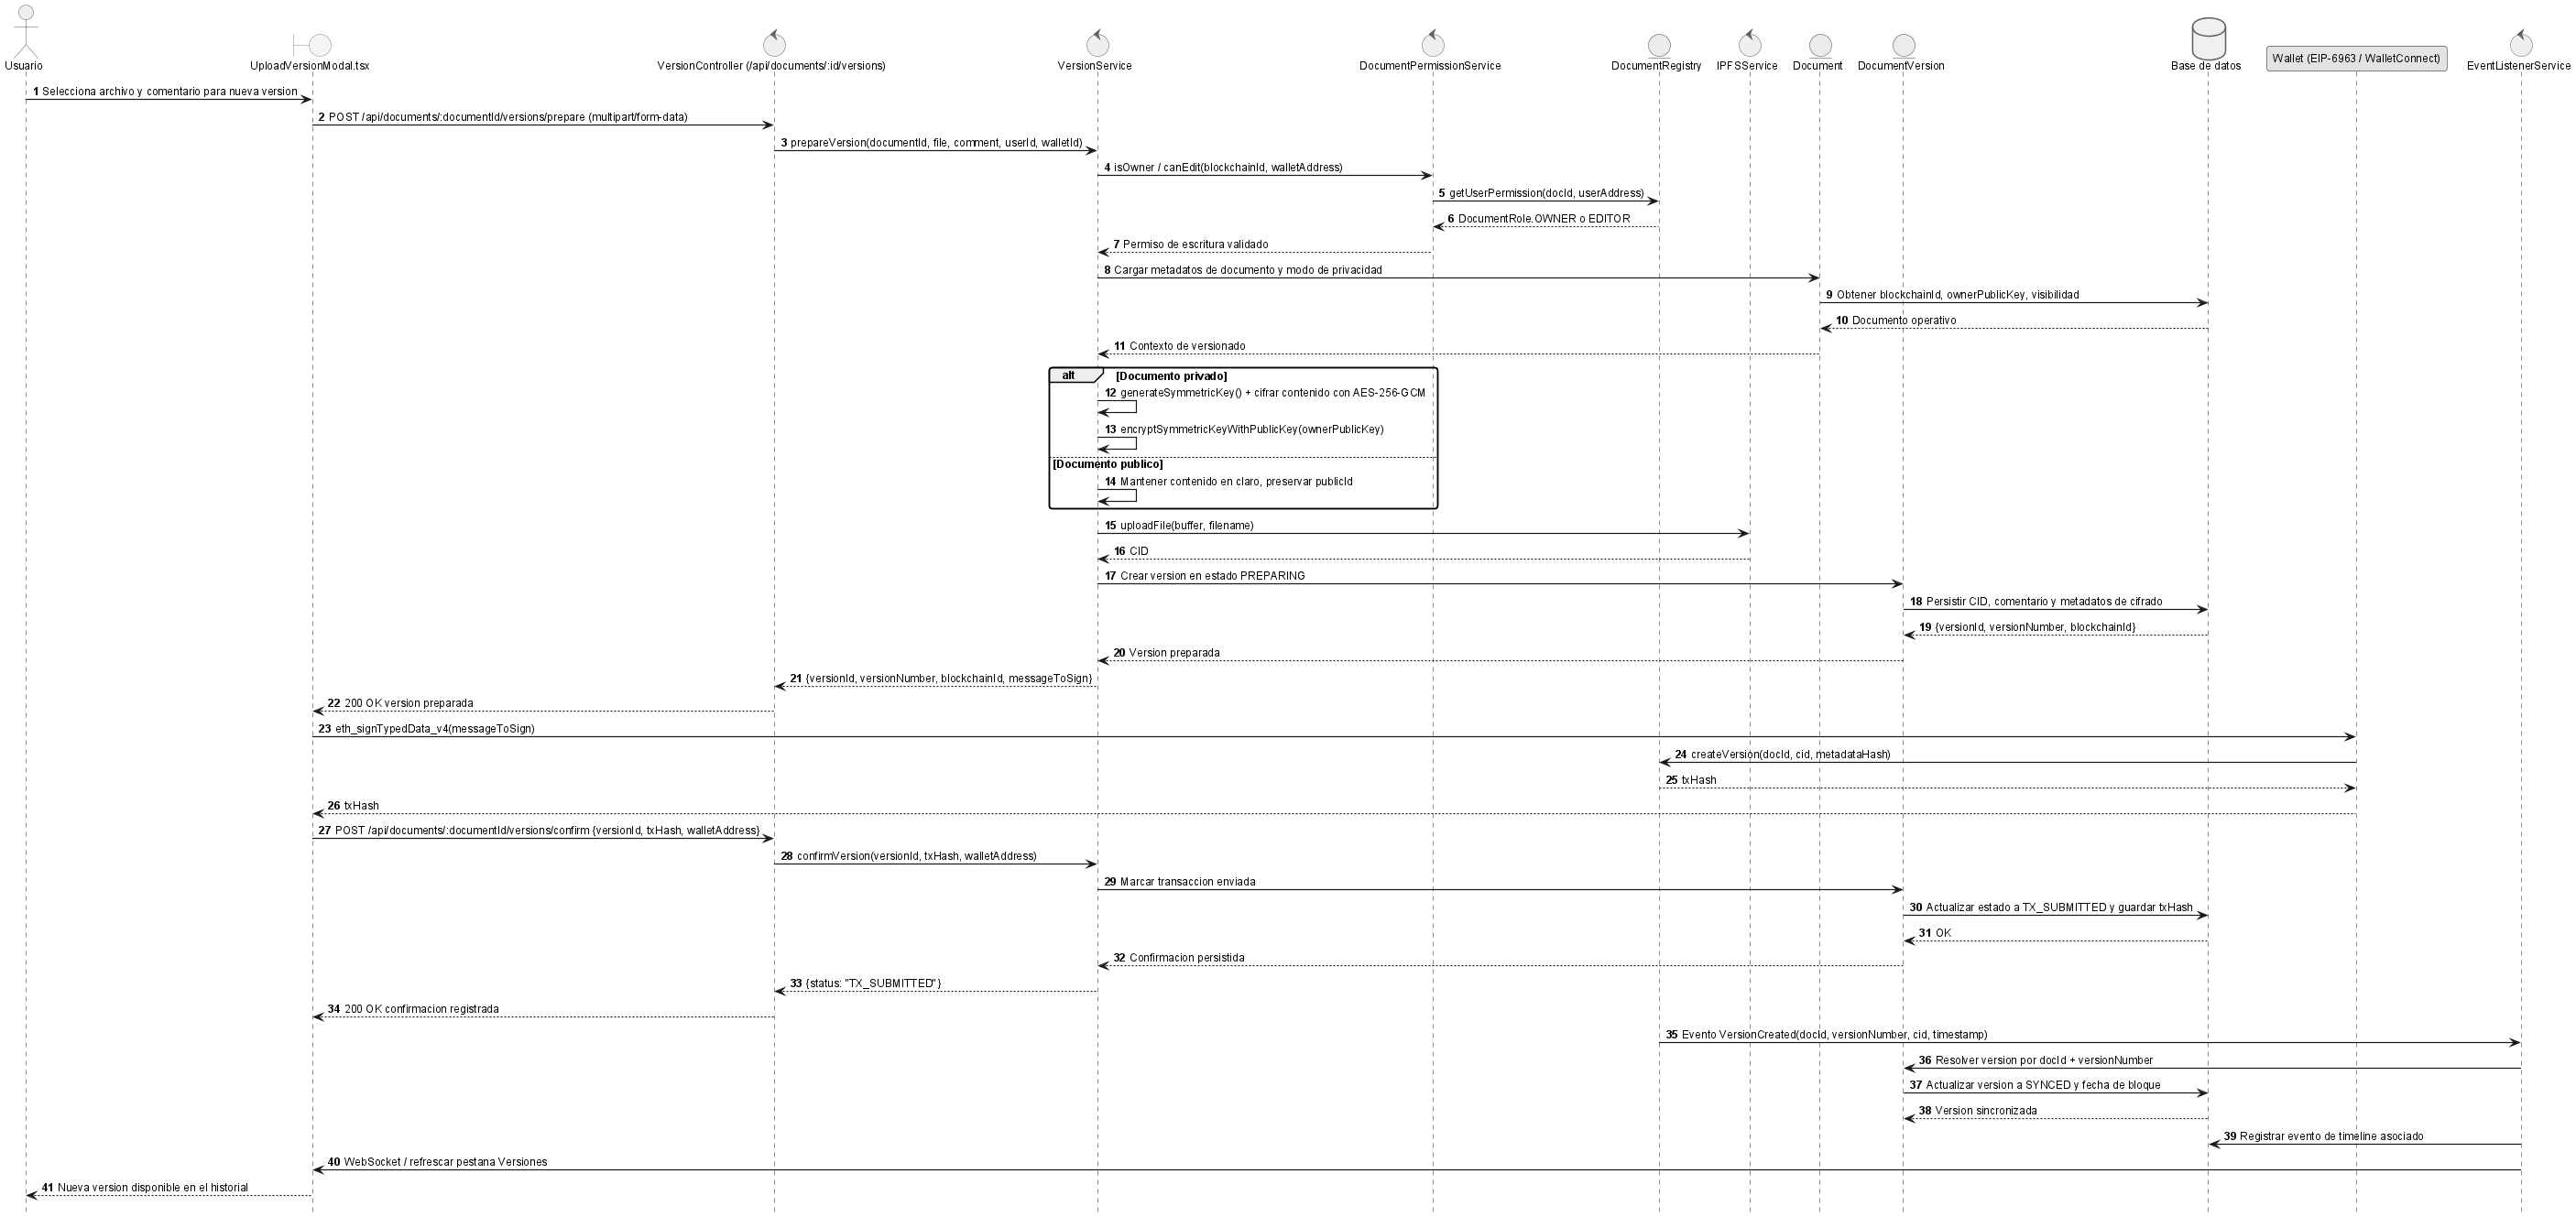
\includegraphics[width=0.9\textwidth]{diagramas/seq-version.png}
    \caption{Diagrama de secuencia UC-0029: Crear Nueva Versión}
    \label{fig:seq-version}
\end{figure}
\subsubsection{Secuencia: Listar Versiones}

\begin{figure}[H]
    \centering
    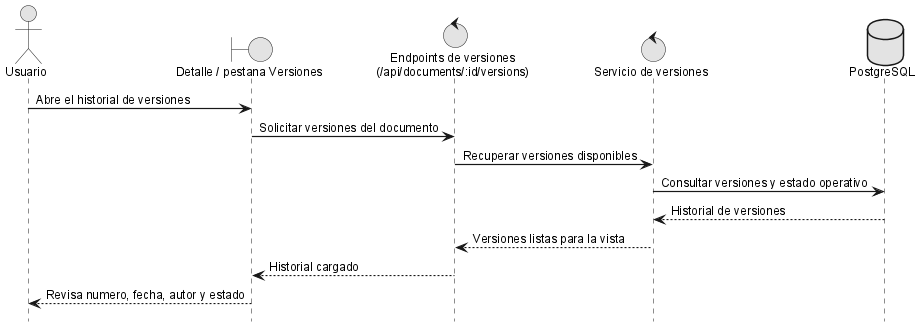
\includegraphics[width=0.9\textwidth]{diagramas/seq-list-versions.png}
    \caption{Diagrama de secuencia UC-0030: Listar Versiones}
    \label{fig:seq-list-versions}
\end{figure}

\subsubsection{Secuencia: Establecer Versión Operativa}

\begin{figure}[H]
    \centering
    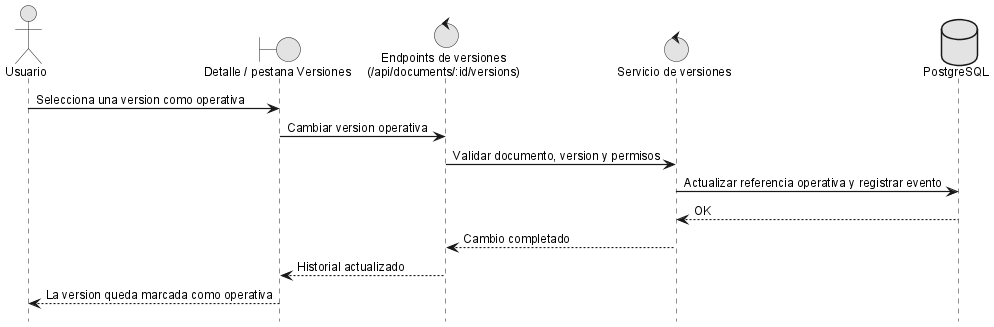
\includegraphics[width=0.9\textwidth]{diagramas/seq-activate-version.png}
    \caption{Diagrama de secuencia UC-0031: Establecer Versión Operativa}
    \label{fig:seq-activate-version}
\end{figure}

\subsubsection{Secuencia: Restaurar Versión Anterior}

\begin{figure}[H]
    \centering
    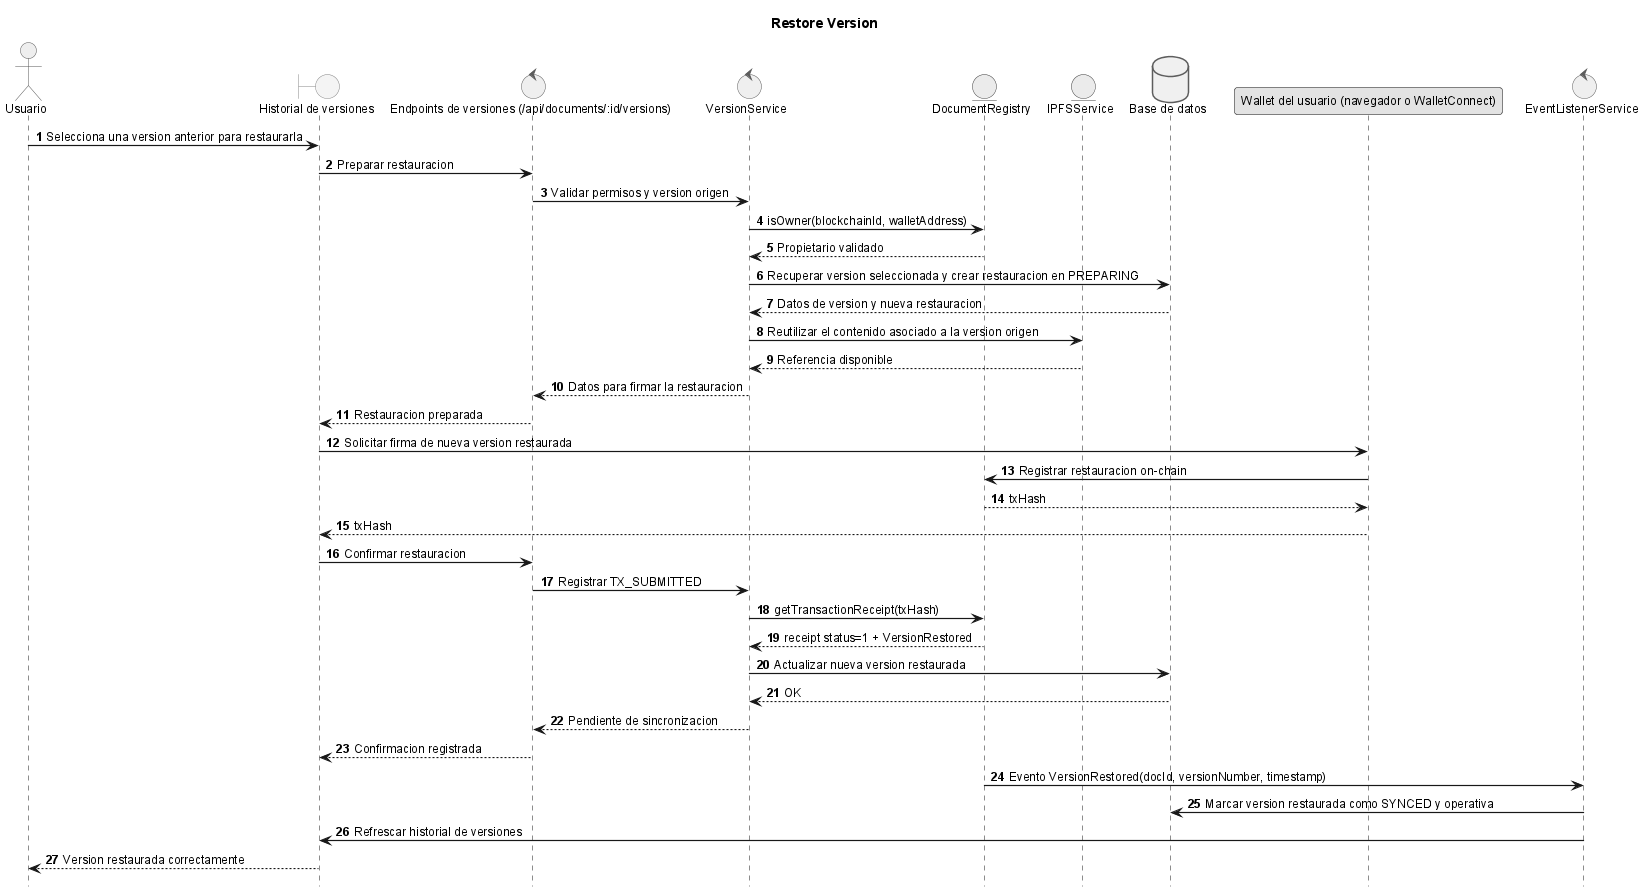
\includegraphics[width=0.9\textwidth]{diagramas/seq-restore-version.png}
    \caption{Diagrama de secuencia UC-0032: Restaurar Versión Anterior}
    \label{fig:seq-restore-version}
\end{figure}

\subsubsection{Secuencia: Descargar Versión Específica}

\begin{figure}[H]
    \centering
    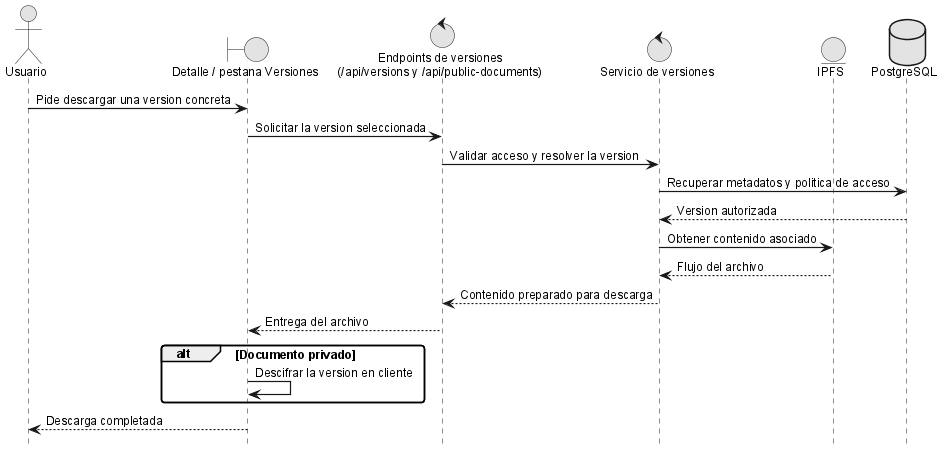
\includegraphics[width=0.9\textwidth]{diagramas/seq-download-version.png}
    \caption{Diagrama de secuencia UC-0033: Descargar Versión Específica}
    \label{fig:seq-download-version}
\end{figure}

\subsubsection{Secuencia: Firmar Documento}

\begin{figure}[H]
    \centering
    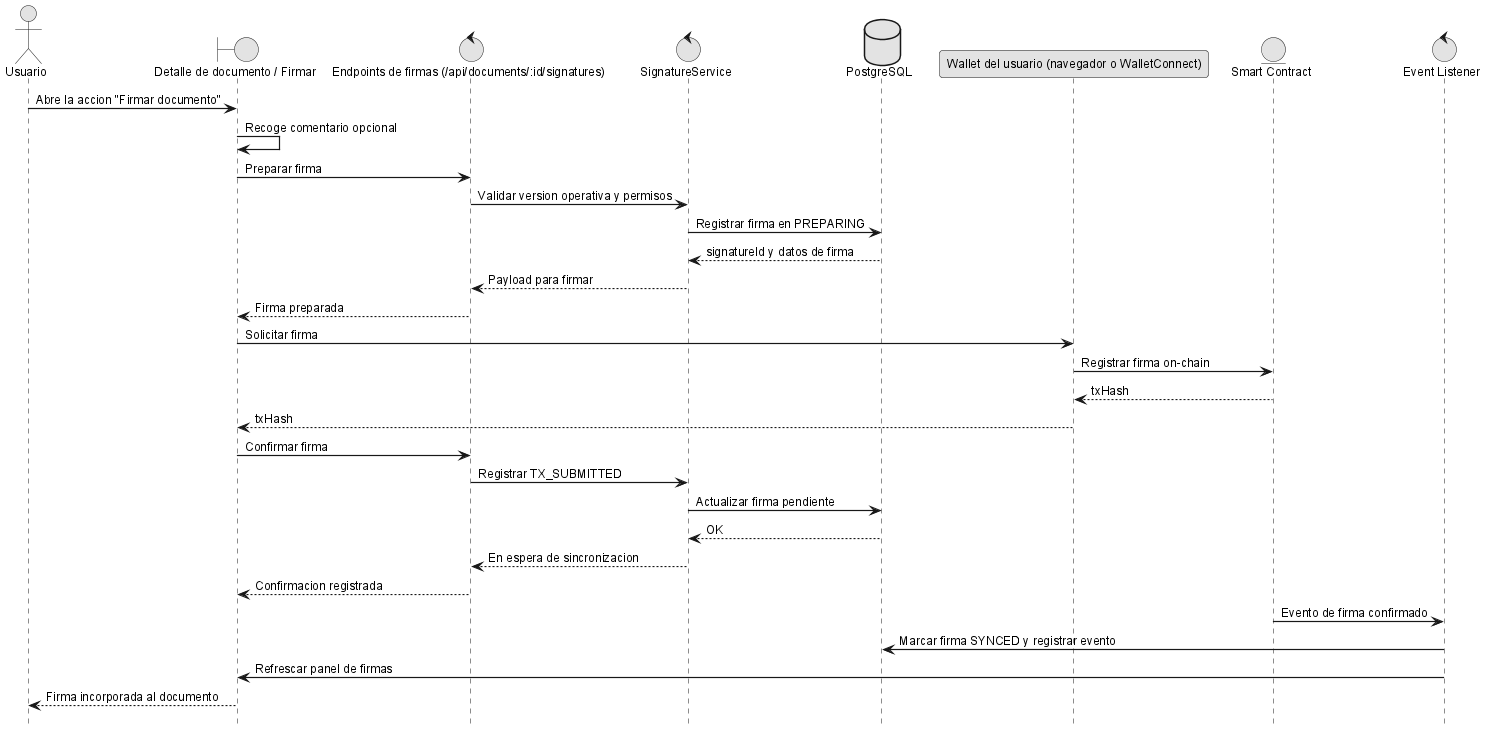
\includegraphics[width=0.9\textwidth]{diagramas/seq-sign.png}
    \caption{Diagrama de secuencia UC-0034: Firmar Documento}
    \label{fig:seq-sign}
\end{figure}

\subsubsection{Secuencia: Ver Firmas de un Documento}

\begin{figure}[H]
    \centering
    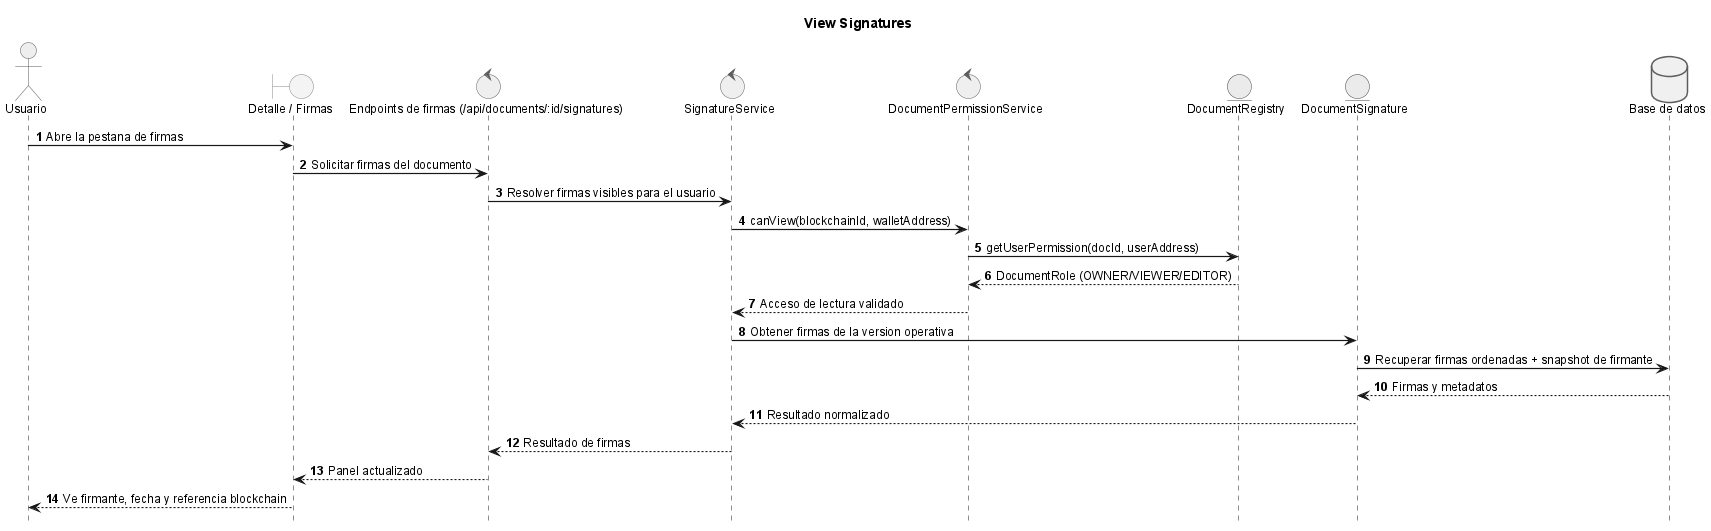
\includegraphics[width=0.9\textwidth]{diagramas/seq-view-signatures.png}
    \caption{Diagrama de secuencia UC-0035: Ver Firmas de un Documento}
    \label{fig:seq-view-signatures}
\end{figure}

\subsubsection{Secuencia: Verificar Firma en Blockchain}

\begin{figure}[H]
    \centering
    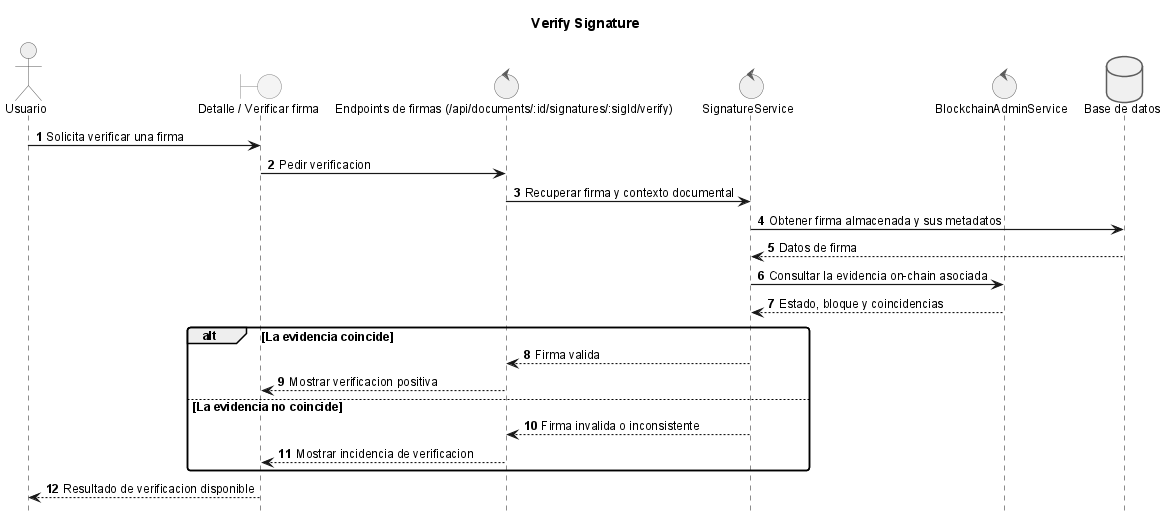
\includegraphics[width=0.9\textwidth]{diagramas/seq-verify-signature.png}
    \caption{Diagrama de secuencia UC-0036: Verificar Firma en Blockchain}
    \label{fig:seq-verify-signature}
\end{figure}

\subsubsection{Secuencia: Compartir Documento}

\begin{figure}[H]
    \centering
    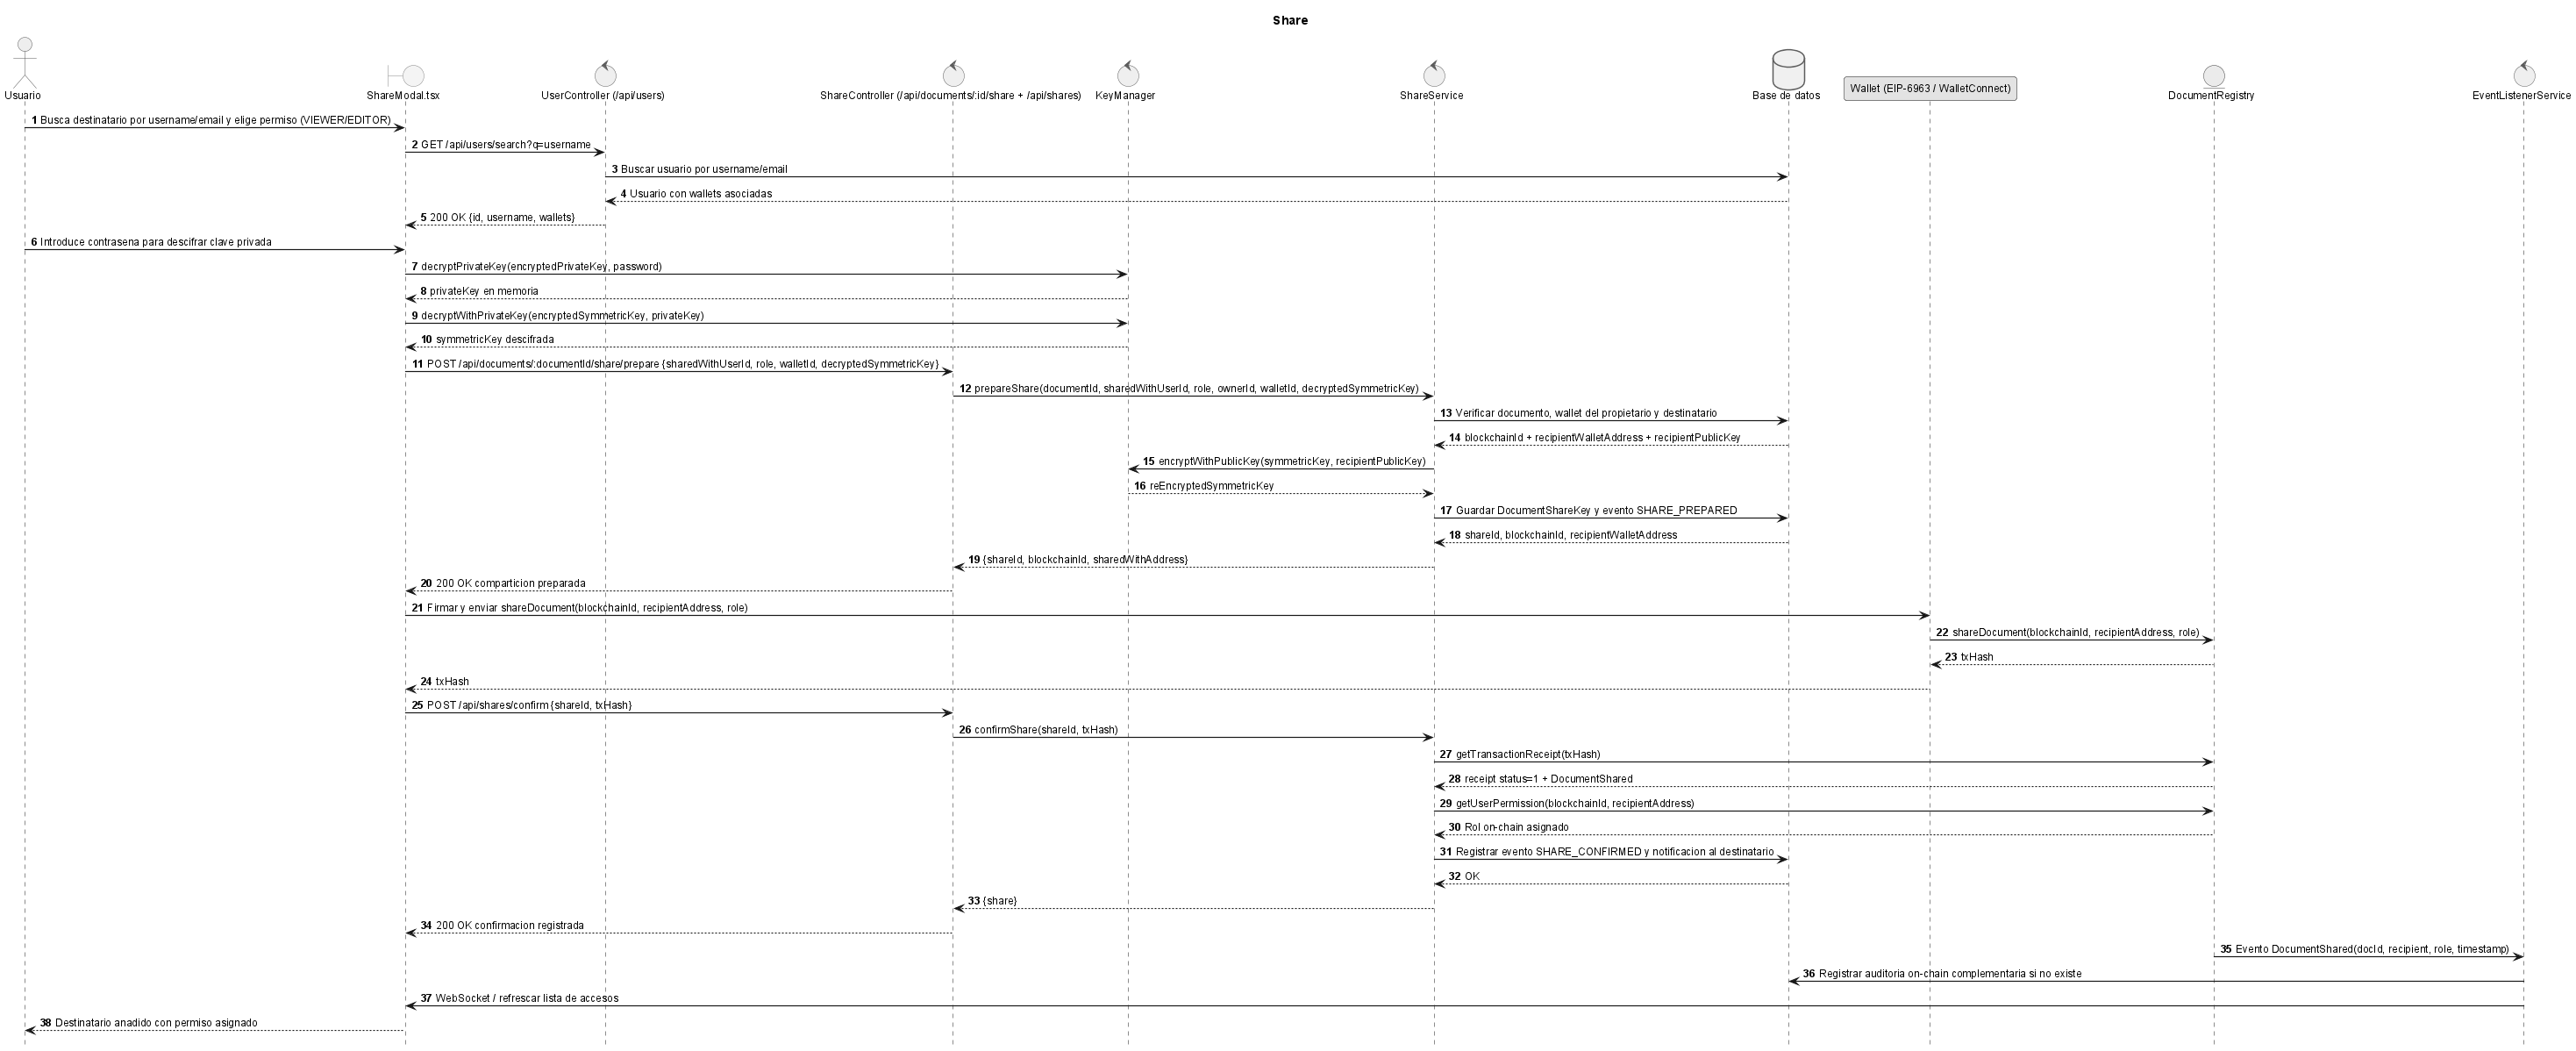
\includegraphics[width=0.9\textwidth]{diagramas/seq-share.png}
    \caption{Diagrama de secuencia UC-0037: Compartir Documento}
    \label{fig:seq-share}
\end{figure}

\subsubsection{Secuencia: Modificar Permisos de Acceso}

Este flujo se conserva como diseño objetivo, pero no forma parte de la interfaz operativa entregada en esta versión. En la aplicación actual el cambio efectivo de nivel de acceso se resuelve revocando el permiso existente y realizando una nueva compartición con el rol deseado.

\begin{figure}[H]
    \centering
    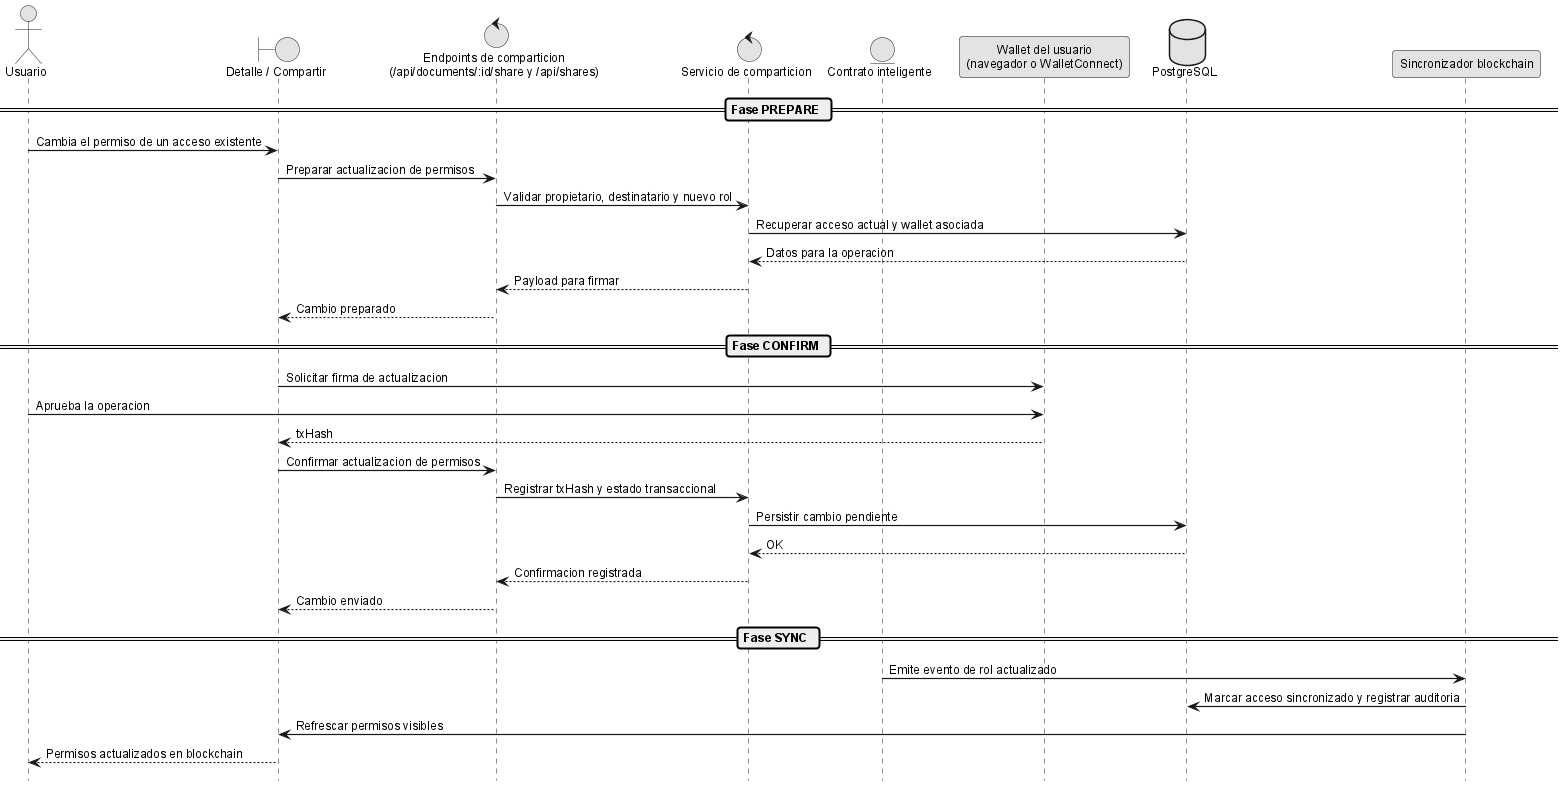
\includegraphics[width=0.9\textwidth]{diagramas/seq-modify-permissions.png}
    \caption{Diagrama de secuencia UC-0038: Modificar Permisos de Acceso}
    \label{fig:seq-modify-permissions}
\end{figure}

\subsubsection{Secuencia: Revocar Acceso a Documento}

\begin{figure}[H]
    \centering
    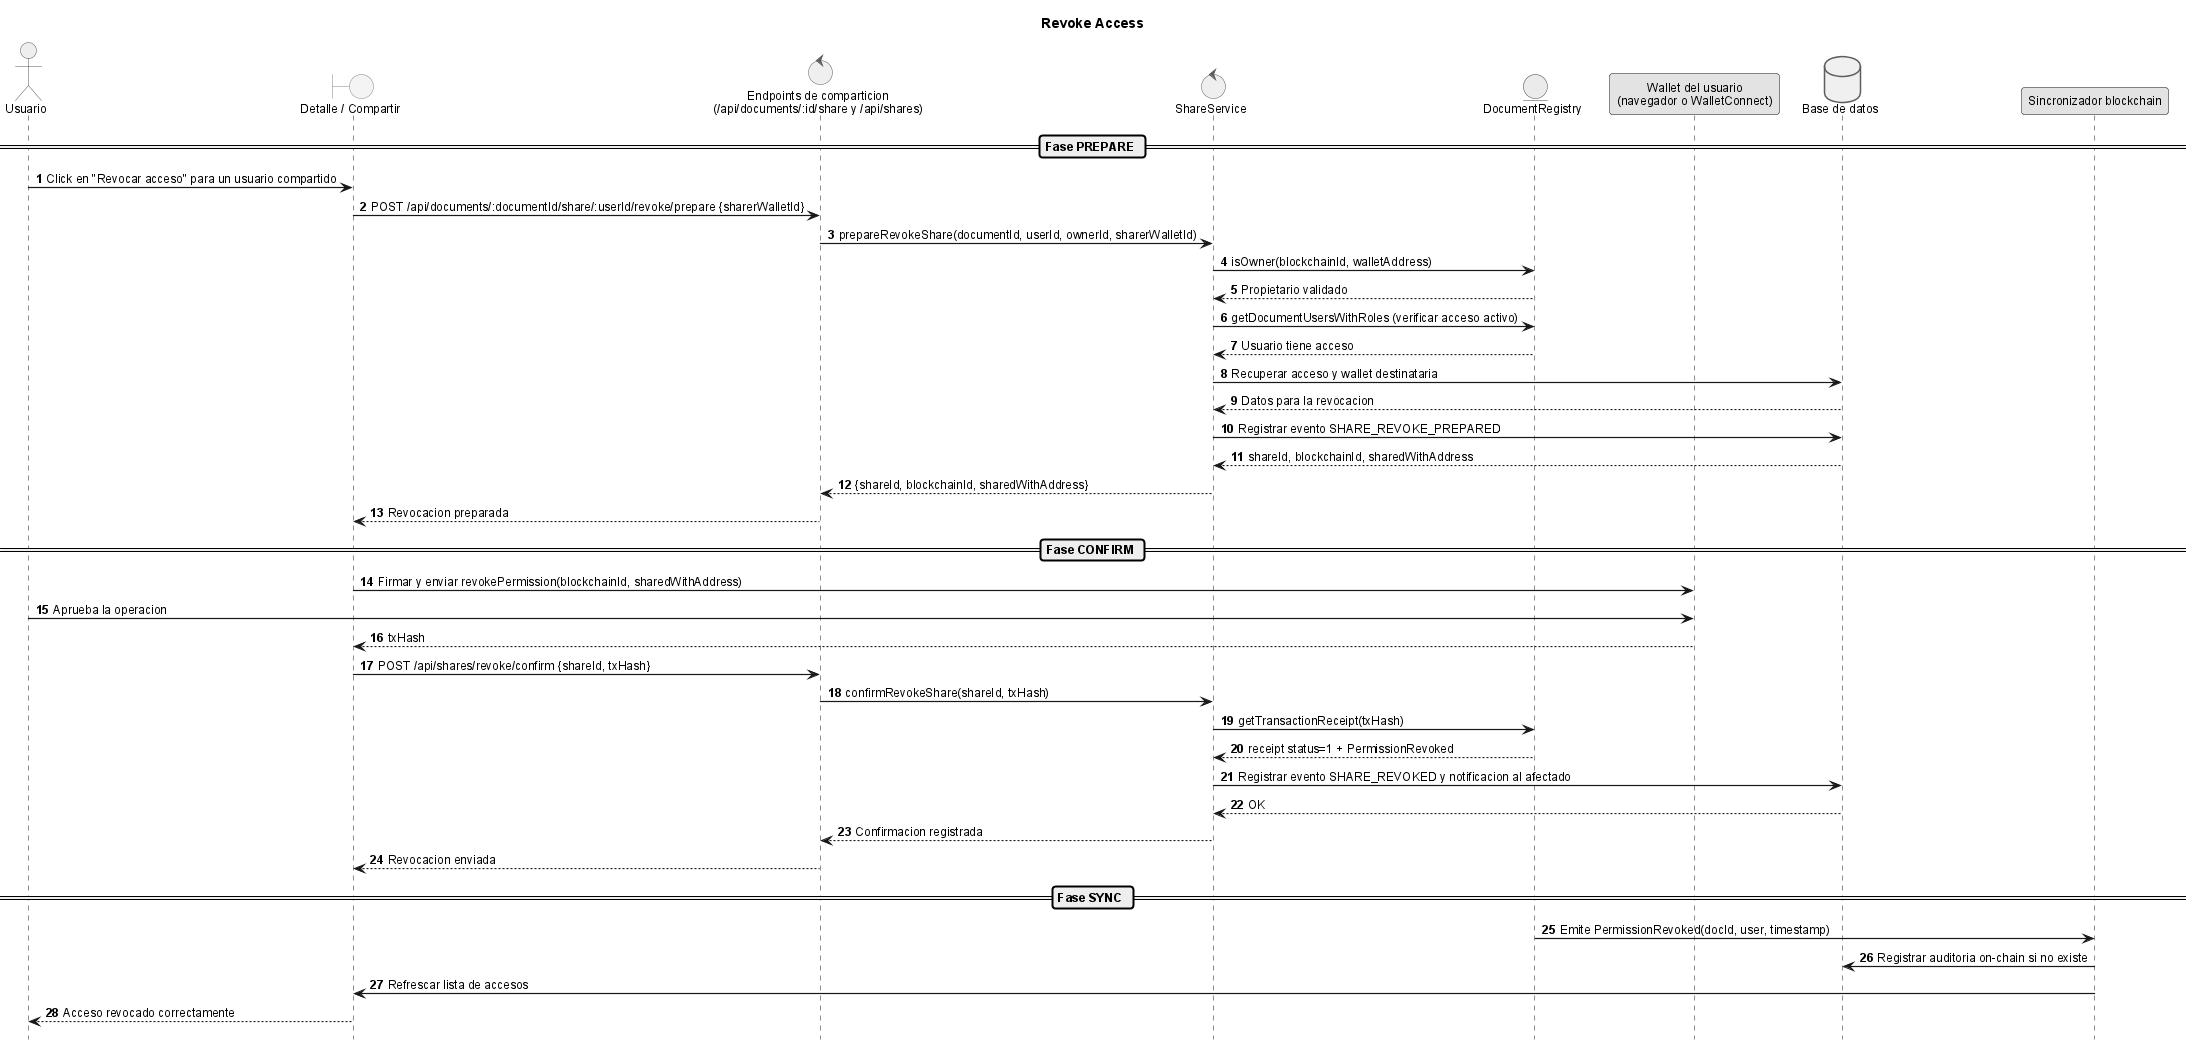
\includegraphics[width=0.9\textwidth]{diagramas/seq-revoke-access.png}
    \caption{Diagrama de secuencia UC-0039: Revocar Acceso a Documento}
    \label{fig:seq-revoke-access}
\end{figure}

\subsubsection{Secuencia: Ver Documentos Compartidos Conmigo}

\begin{figure}[H]
    \centering
    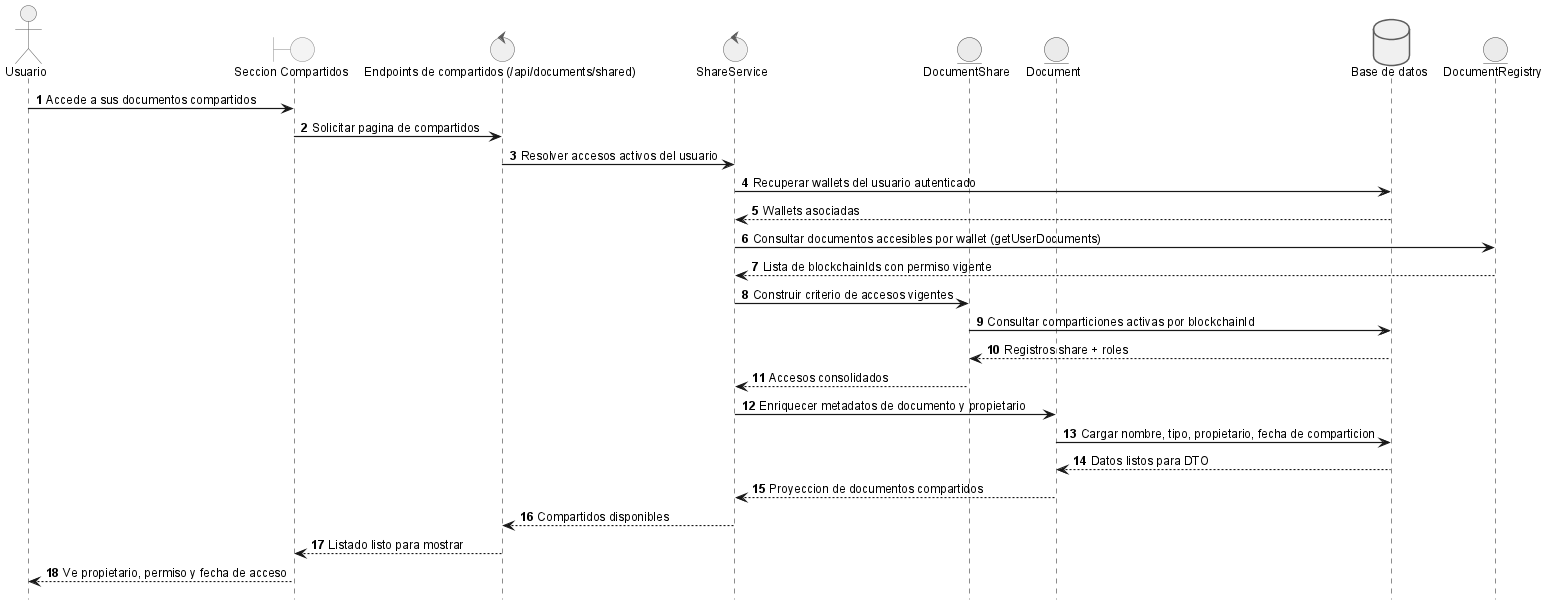
\includegraphics[width=0.9\textwidth]{diagramas/seq-shared-documents.png}
    \caption{Diagrama de secuencia UC-0040: Ver Documentos Compartidos Conmigo}
    \label{fig:seq-shared-documents}
\end{figure}

\subsubsection{Secuencia: Gestionar Carpetas}

\begin{figure}[H]
    \centering
    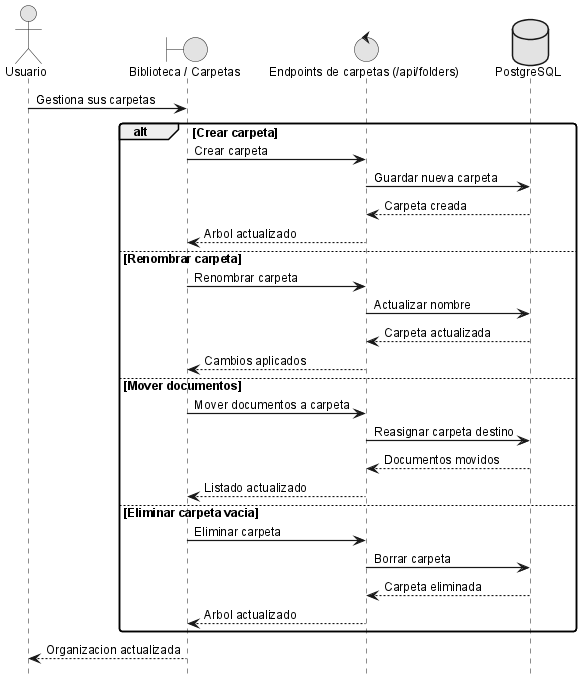
\includegraphics[width=0.9\textwidth]{diagramas/seq-create-folder.png}
    \caption{Diagrama de secuencia UC-0041: Gestionar Carpetas}
    \label{fig:seq-create-folder}
\end{figure}

\subsubsection{Secuencia: Gestionar Categorías}

\begin{figure}[H]
    \centering
    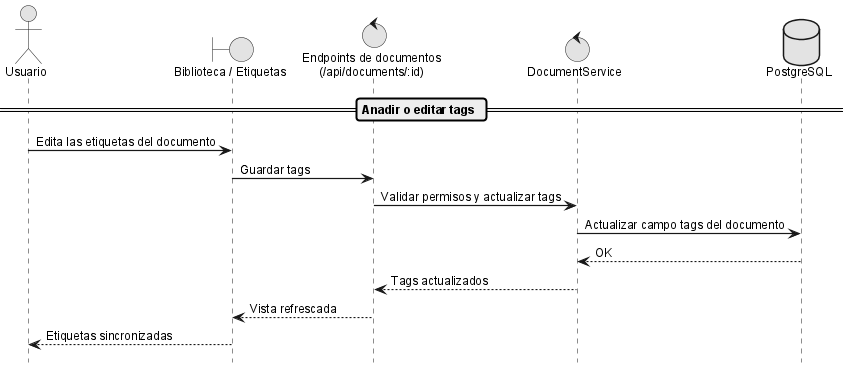
\includegraphics[width=0.9\textwidth]{diagramas/seq-categories.png}
    \caption{Diagrama de secuencia UC-0042: Gestionar Categorías}
    \label{fig:seq-categories}
\end{figure}

\subsubsection{Secuencia: Etiquetar Documento}

\begin{figure}[H]
    \centering
    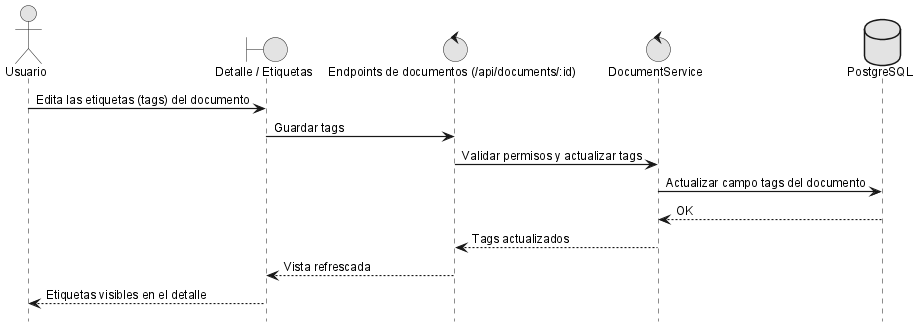
\includegraphics[width=0.9\textwidth]{diagramas/seq-tag-document.png}
    \caption{Diagrama de secuencia UC-0043: Etiquetar Documento}
    \label{fig:seq-tag-document}
\end{figure}

\subsubsection{Secuencia: Ver Timeline de Documento}

\begin{figure}[H]
    \centering
    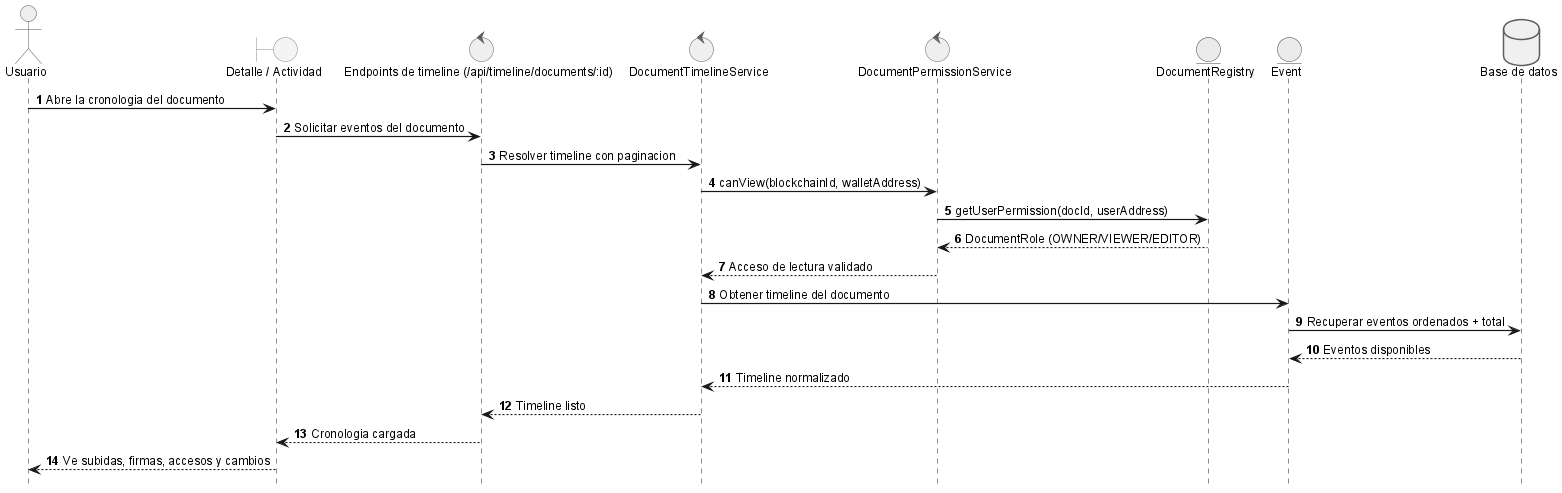
\includegraphics[width=0.9\textwidth]{diagramas/seq-timeline.png}
    \caption{Diagrama de secuencia UC-0044: Ver Timeline de Documento}
    \label{fig:seq-timeline}
\end{figure}

\subsubsection{Secuencia: Ver Estadísticas Personales}

\begin{figure}[H]
    \centering
    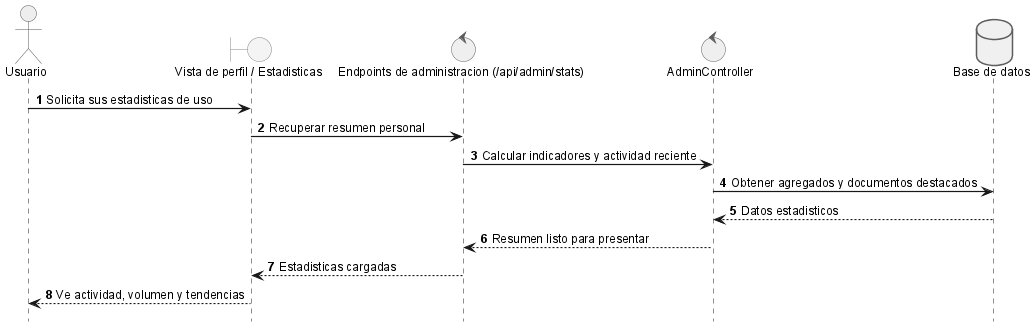
\includegraphics[width=0.9\textwidth]{diagramas/seq-user-stats.png}
    \caption{Diagrama de secuencia UC-0045: Ver Estadísticas Personales}
    \label{fig:seq-user-stats}
\end{figure}

\subsubsection{Secuencia: Ver Estadísticas Globales del Sistema}

\begin{figure}[H]
    \centering
    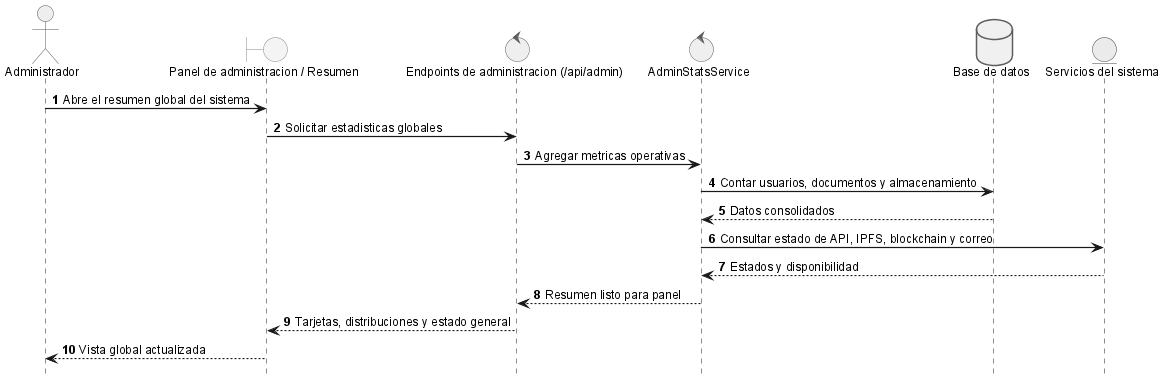
\includegraphics[width=0.9\textwidth]{diagramas/seq-global-stats.png}
    \caption{Diagrama de secuencia UC-0046: Ver Estadísticas Globales del Sistema}
    \label{fig:seq-global-stats}
\end{figure}
%
% === fin PlantUML ===

\begin{figure}[H]
    \centering
    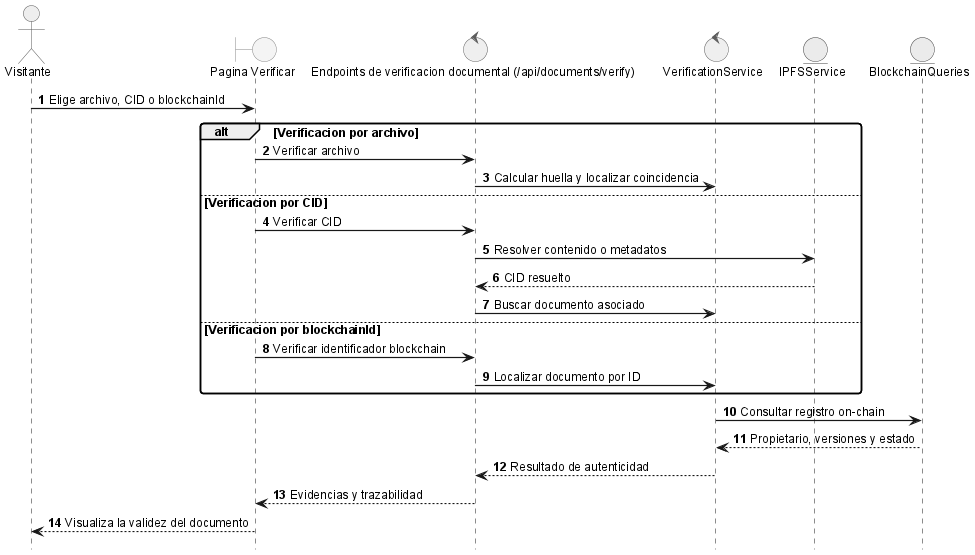
\includegraphics[width=0.9\textwidth]{diagramas/seq-verify-authenticity.png}
    \caption{Diagrama de secuencia UC-0047: Verificar Autenticidad de Documento}
    \label{fig:seq-verify-authenticity}
\end{figure}

\subsubsection{Secuencia: Auditoría Blockchain}

\begin{figure}[H]
    \centering
    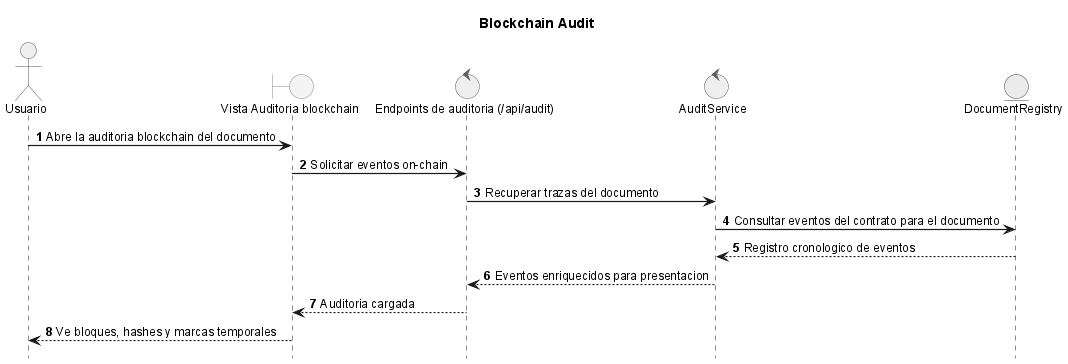
\includegraphics[width=0.9\textwidth]{diagramas/seq-blockchain-audit.png}
    \caption{Diagrama de secuencia UC-0048: Auditoría Blockchain}
    \label{fig:seq-blockchain-audit}
\end{figure}

\subsubsection{Secuencia: Listar Usuarios (Admin)}

\begin{figure}[H]
    \centering
    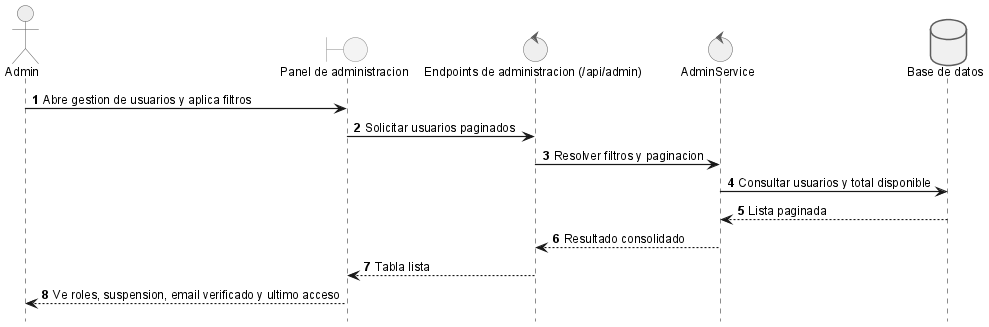
\includegraphics[width=0.9\textwidth]{diagramas/seq-list-users.png}
    \caption{Diagrama de secuencia UC-0049: Listar Usuarios}
    \label{fig:seq-list-users}
\end{figure}

\subsubsection{Secuencia: Gestionar Roles de Usuario}

\begin{figure}[H]
    \centering
    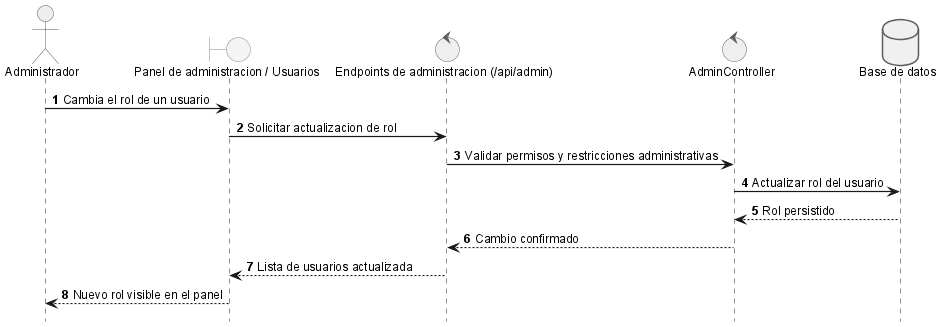
\includegraphics[width=0.9\textwidth]{diagramas/seq-manage-roles.png}
    \caption{Diagrama de secuencia UC-0050: Gestionar Roles de Usuario}
    \label{fig:seq-manage-roles}
\end{figure}
%
% === fin PlantUML ===

\begin{figure}[H]
    \centering
    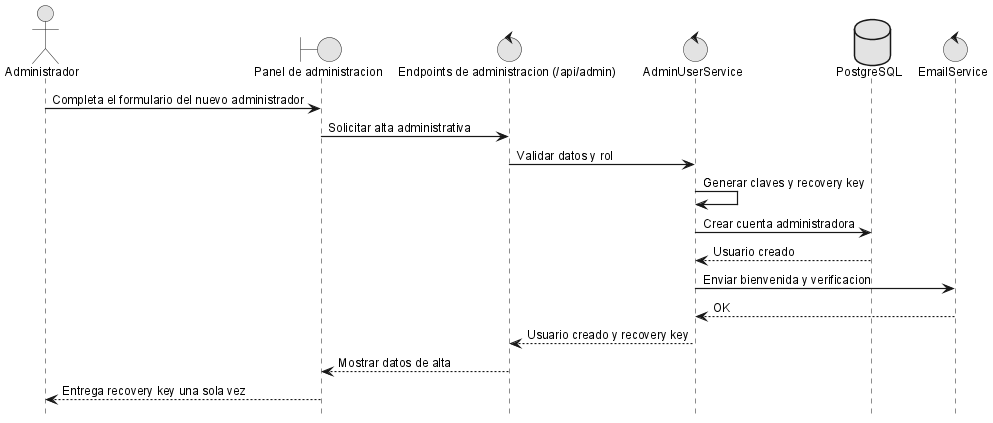
\includegraphics[width=0.9\textwidth]{diagramas/seq-create-admin.png}
    \caption{Diagrama de secuencia UC-0051: Crear Usuario Administrador}
    \label{fig:seq-create-admin}
\end{figure}

\subsubsection{Secuencia: Suspender Usuario (Admin)}

\begin{figure}[H]
    \centering
    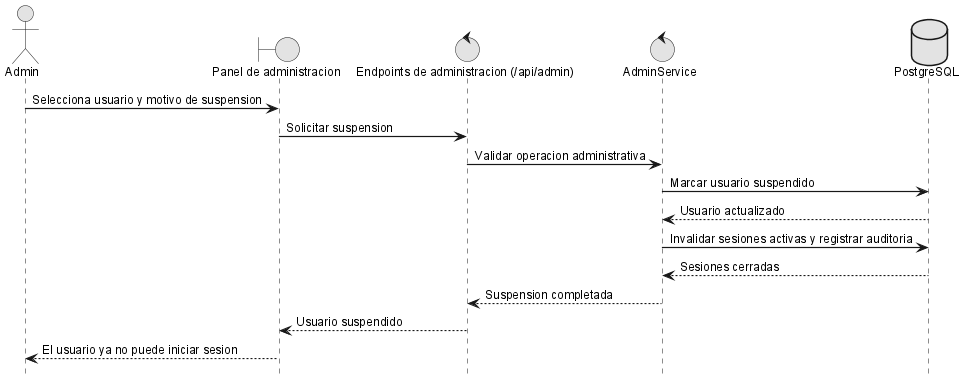
\includegraphics[width=0.9\textwidth]{diagramas/seq-suspend-user.png}
    \caption{Diagrama de secuencia UC-0052: Suspender Usuario}
    \label{fig:seq-suspend-user}
\end{figure}

\subsubsection{Secuencia: Eliminar Cuenta de Usuario (Admin)}

% === PlantUML source (comentado) ===
% @startuml
% skinparam sequenceArrowThickness 2
% skinparam roundcorner 5
% skinparam sequenceParticipant underline
% skinparam monochrome true
%
% actor "Administrador" as ADMIN
% boundary "Frontend Admin" as FE
% control "AdminController" as AC
% entity "AdminUserService" as AUS
% entity "UserRepository" as UR
% entity "BlockchainAdminService" as BAS
%
% ADMIN -> FE: Selecciona usuario y pulsa Eliminar cuenta
% FE -> FE: Muestra advertencia de irreversibilidad
% ADMIN -> FE: Confirma la eliminacion
% FE -> AC: DELETE /api/admin/users/:userId
% AC -> AUS: checkNotSelfDelete(adminId, userId)
% AUS --> AC: OK (no es auto-eliminacion)
% AC -> AUS: deleteUser(userId)
% AUS -> UR: deleteUserCascade(userId)
% note right of UR
%   Elimina en cascada:
%   sessions, tokens, wallets,
%   firmas, comparticiones,
%   documentos propios
% end note
% UR --> AUS: usuario eliminado
% AUS -> BAS: revokeAllWallets(userId)
% BAS --> AUS: OK
% AUS --> AC: usuario eliminado
% AC --> FE: 200 OK
% FE --> ADMIN: Listado de usuarios actualizado
% @enduml
% === fin PlantUML ===

\begin{figure}[H]
    \centering
    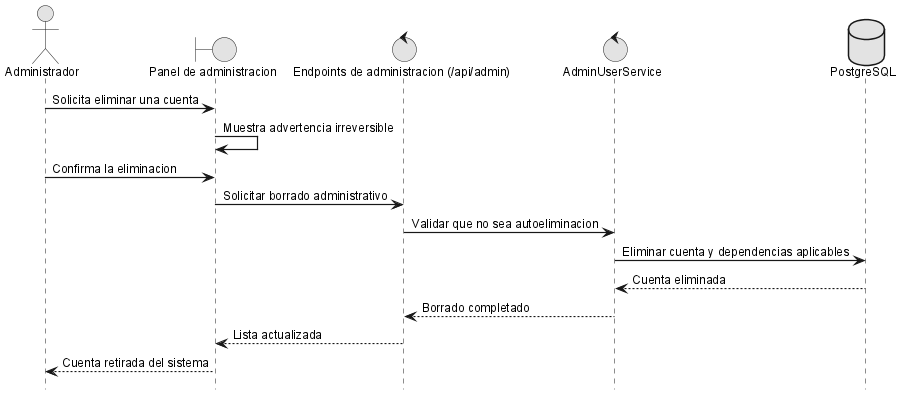
\includegraphics[width=0.9\textwidth]{diagramas/seq-delete-user-admin.png}
    \caption{Diagrama de secuencia UC-0053: Eliminar Cuenta de Usuario (Admin)}
    \label{fig:seq-delete-user-admin}
\end{figure}

\subsubsection{Secuencia: Pausar Sistema (Circuit Breaker)}

\begin{figure}[H]
    \centering
    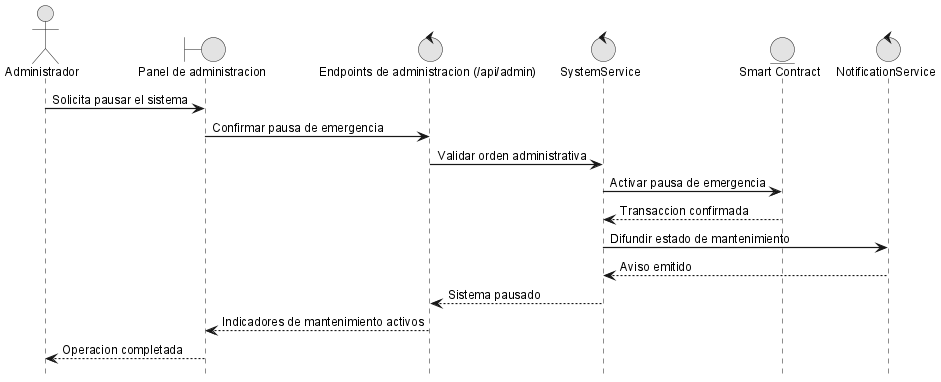
\includegraphics[width=0.9\textwidth]{diagramas/seq-pause-system.png}
    \caption{Diagrama de secuencia UC-0054: Pausar Sistema (Circuit Breaker)}
    \label{fig:seq-pause-system}
\end{figure}
%
% === fin PlantUML ===

\begin{figure}[H]
    \centering
    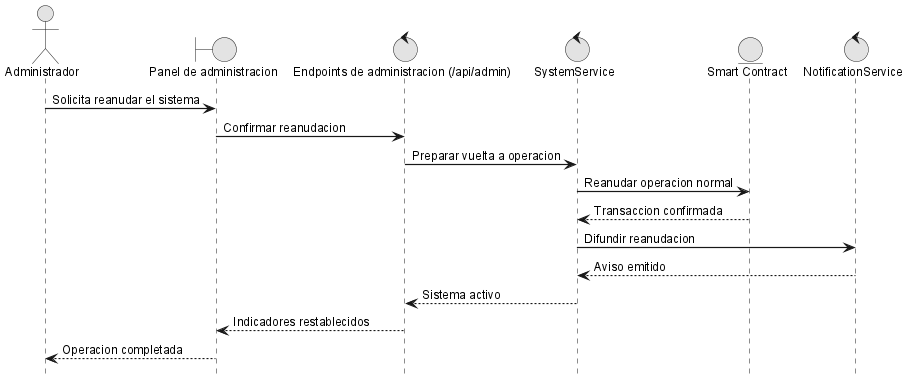
\includegraphics[width=0.9\textwidth]{diagramas/seq-resume-system.png}
    \caption{Diagrama de secuencia UC-0055: Reanudar Sistema}
    \label{fig:seq-resume-system}
\end{figure}

\subsubsection{Secuencia: Ver Notificaciones}

\begin{figure}[H]
    \centering
    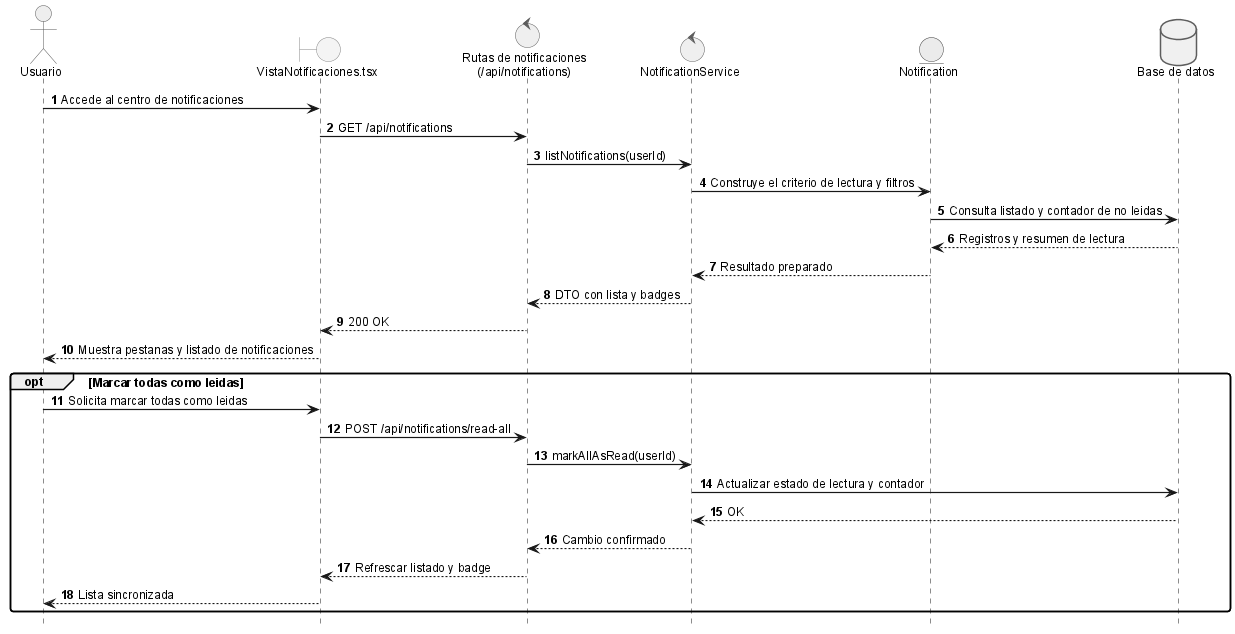
\includegraphics[width=0.9\textwidth]{diagramas/seq-notifications.png}
    \caption{Diagrama de secuencia UC-0056: Ver Notificaciones}
    \label{fig:seq-notifications}
\end{figure}

\subsubsection{Secuencia: Configurar Preferencias de Notificación}

\begin{figure}[H]
    \centering
    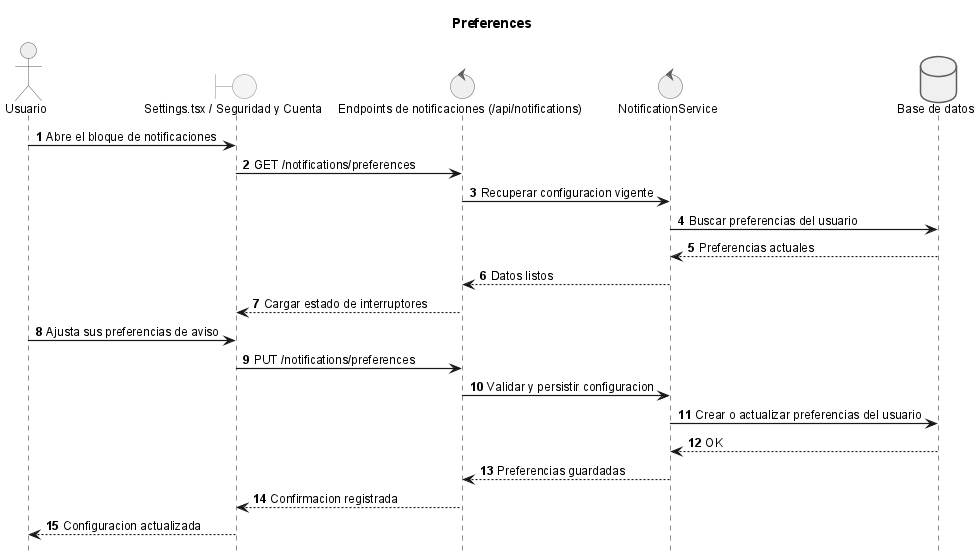
\includegraphics[width=0.9\textwidth]{diagramas/seq-preferences.png}
    \caption{Diagrama de secuencia UC-0057: Configurar Preferencias de Notificación}
    \label{fig:seq-preferences}
\end{figure}

\subsection{Diagramas de caso de uso-diseño}

La numeración de casos de uso concluye en UC-0057. Los diagramas que siguen no introducen nuevos casos de uso, sino variantes y flujos complementarios que detallan escenarios especialmente relevantes dentro de UC ya definidos en el Anexo I. En ellos se enfatiza la participación simultánea de la interfaz, los servicios, la persistencia operativa y la confirmación blockchain.

\subsubsection{Colaboración: UC-0019 Subir Documento}

\begin{figure}[H]
    \centering
    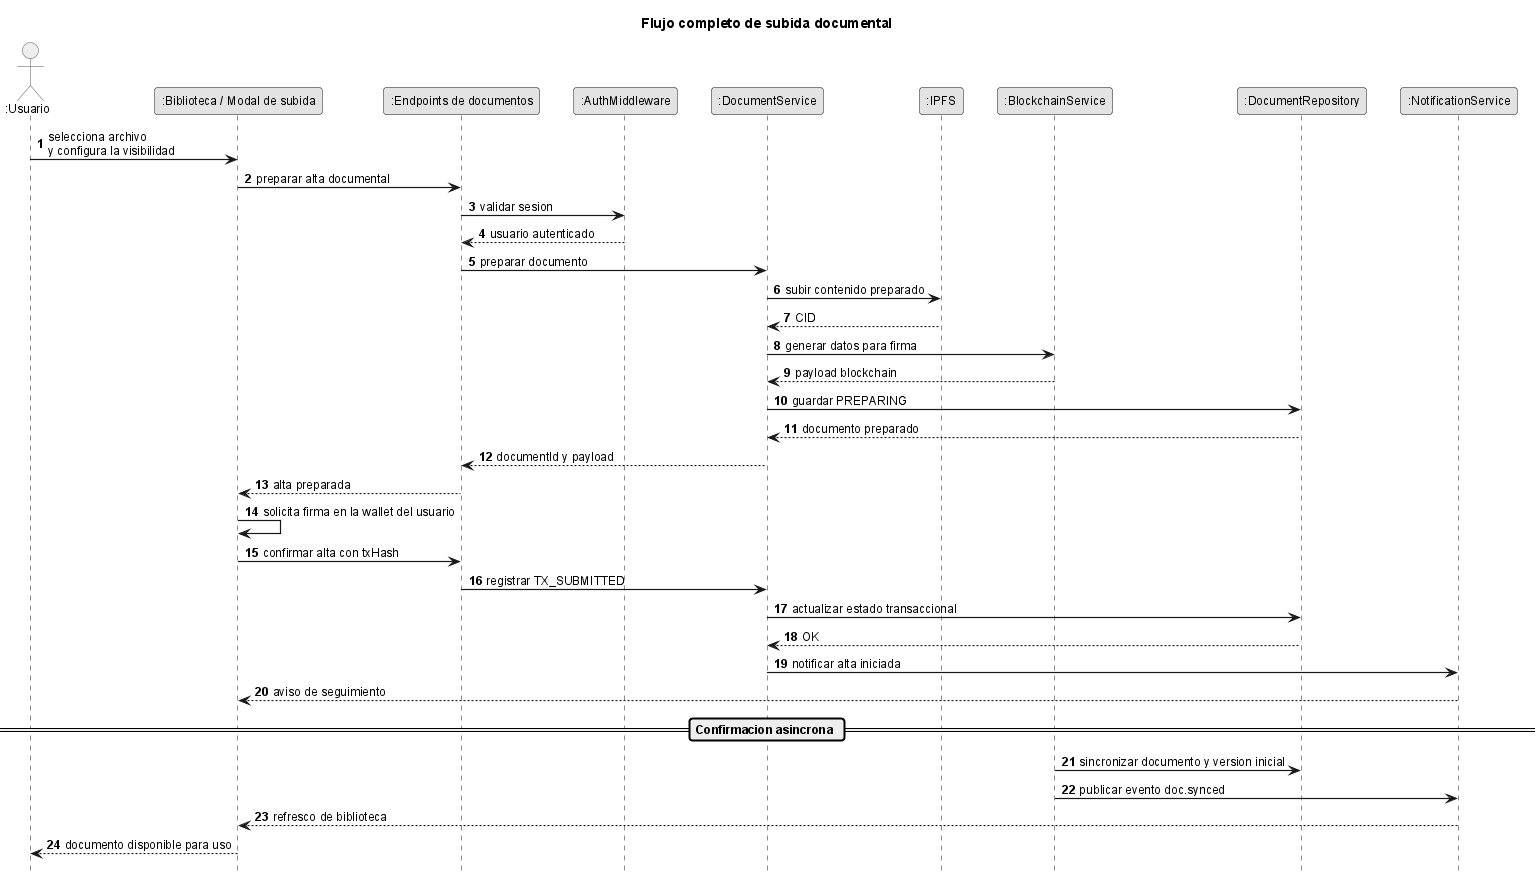
\includegraphics[width=0.92\textwidth]{diagramas/collaboration-upload.png}
    \caption{Diagrama de colaboración para UC-0019: Subir Documento}
    \label{fig:collaboration-upload}
\end{figure}

Este diagrama resume la coordinación entre la interfaz de carga, el backend de documentos, IPFS, PostgreSQL y el contrato inteligente durante el alta inicial de un documento.

\subsubsection{Colaboración: UC-0034 Firmar Documento}

\begin{figure}[H]
    \centering
    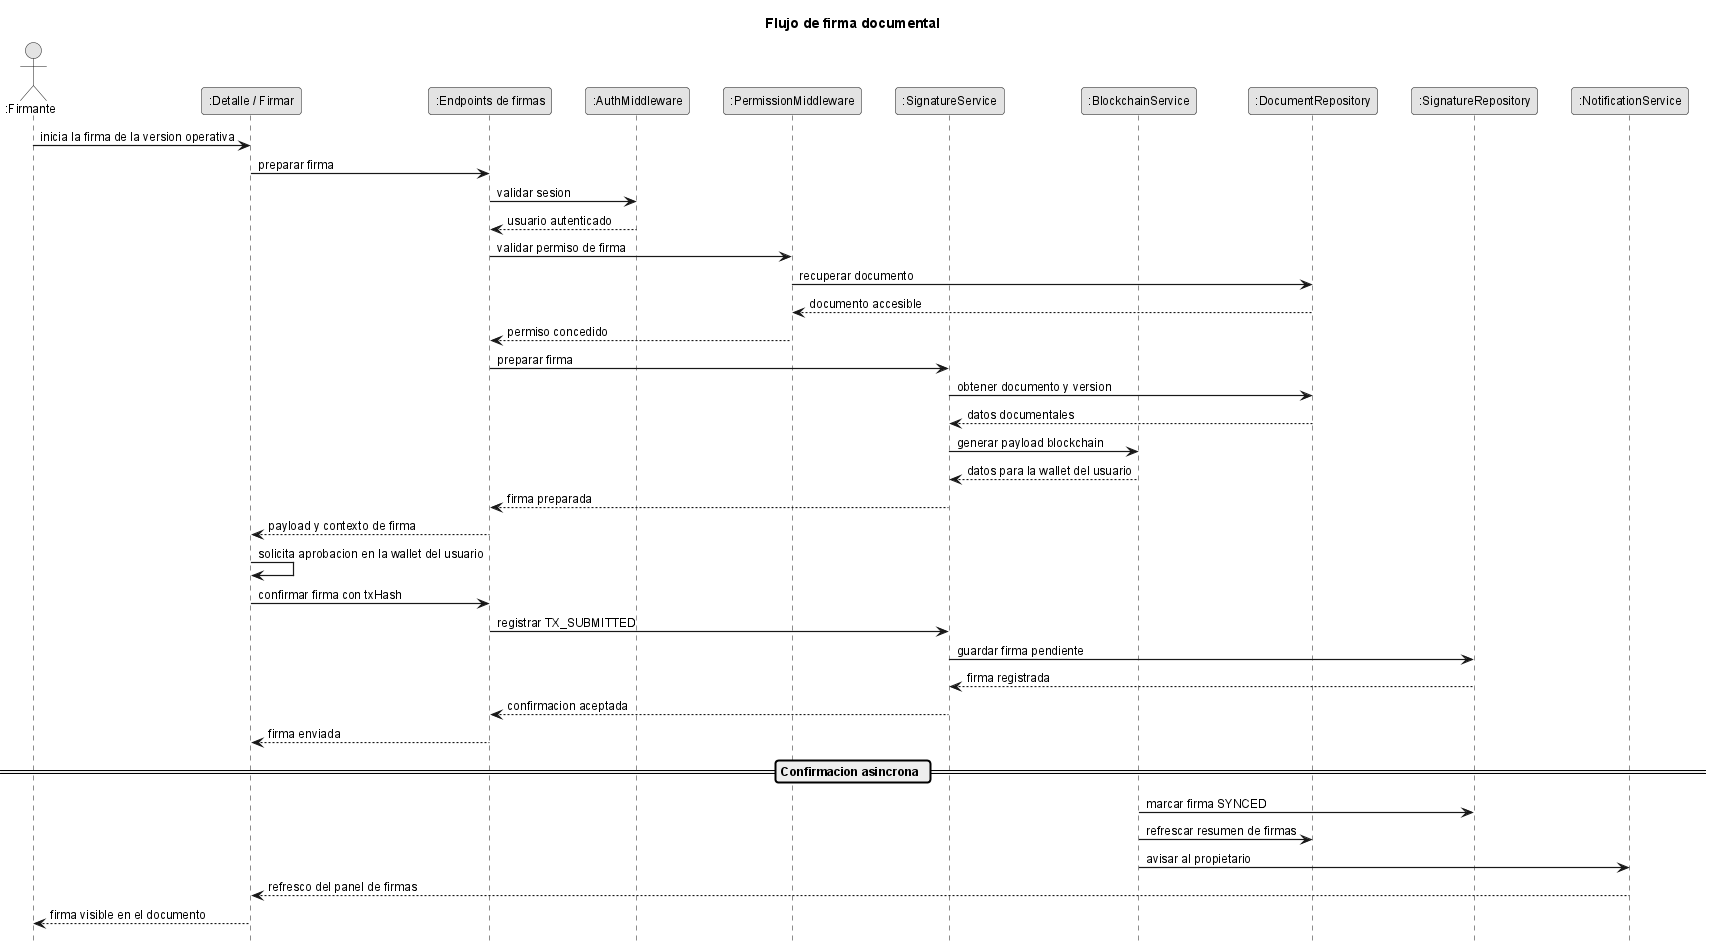
\includegraphics[width=0.92\textwidth]{diagramas/collaboration-sign.png}
    \caption{Diagrama de colaboración para UC-0034: Firmar Documento}
    \label{fig:collaboration-sign}
\end{figure}

El mismo patrón de colaboración se reutiliza en operaciones críticas con firma de wallet, como compartir, transferir o crear nuevas versiones, variando únicamente el servicio de dominio y el evento on-chain confirmado.

\subsubsection{Flujo complementario: Publicación pública durante la subida}

\begin{figure}[H]
    \centering
    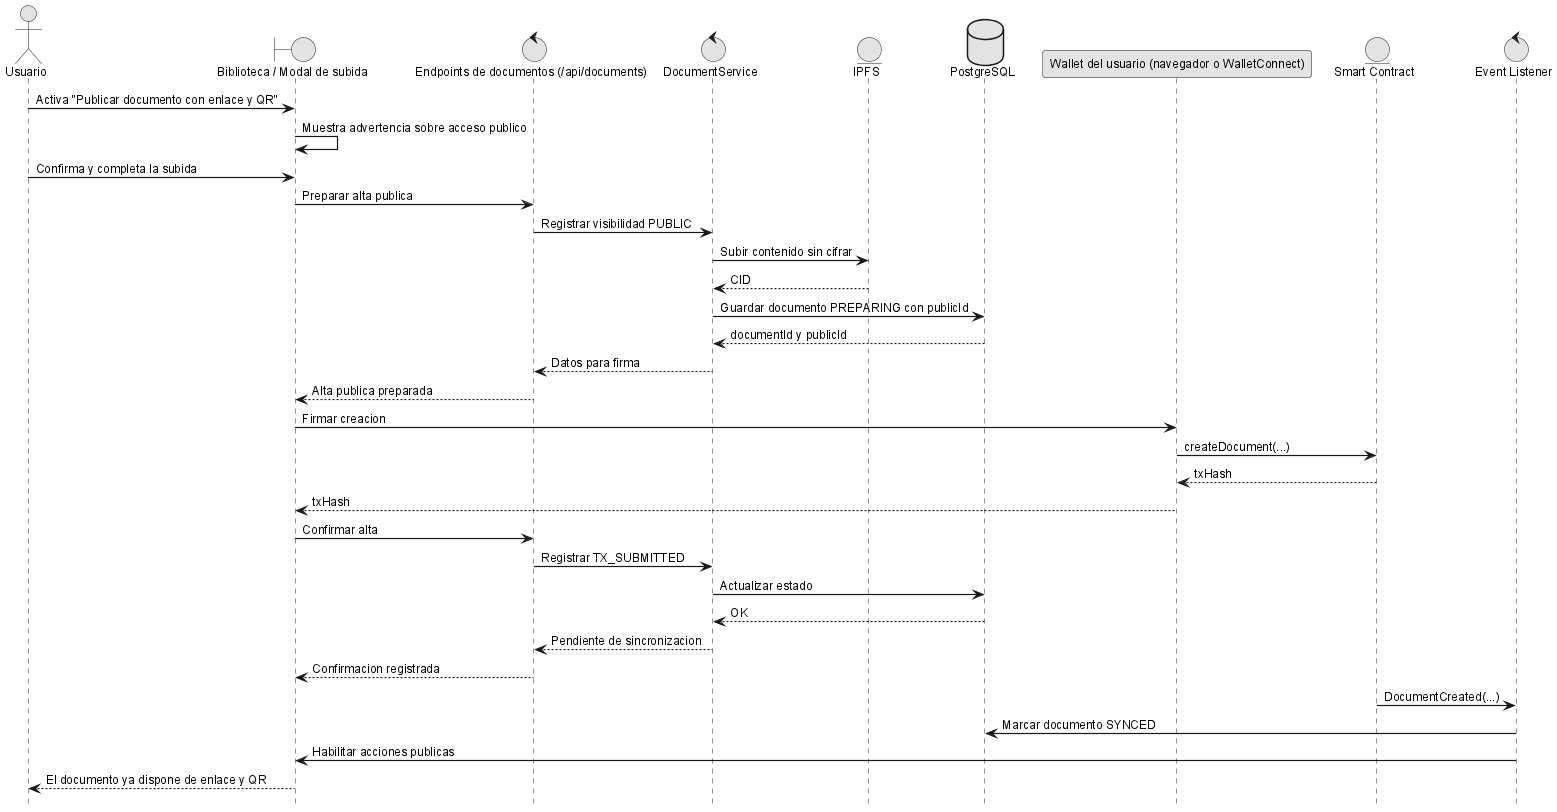
\includegraphics[width=0.92\textwidth]{diagramas/flow-public-upload.png}
    \caption{Flujo complementario de publicación pública integrado en UC-0019}
    \label{fig:flow-public-upload}
\end{figure}

Este flujo desarrolla la variante pública del alta documental: el contenido se publica sin cifrado, se genera un \texttt{publicId} y el acceso compartible queda disponible tras la confirmación de la transacción.

\subsubsection{Flujo complementario: Compartición mediante enlace y código QR}

\begin{figure}[H]
    \centering
    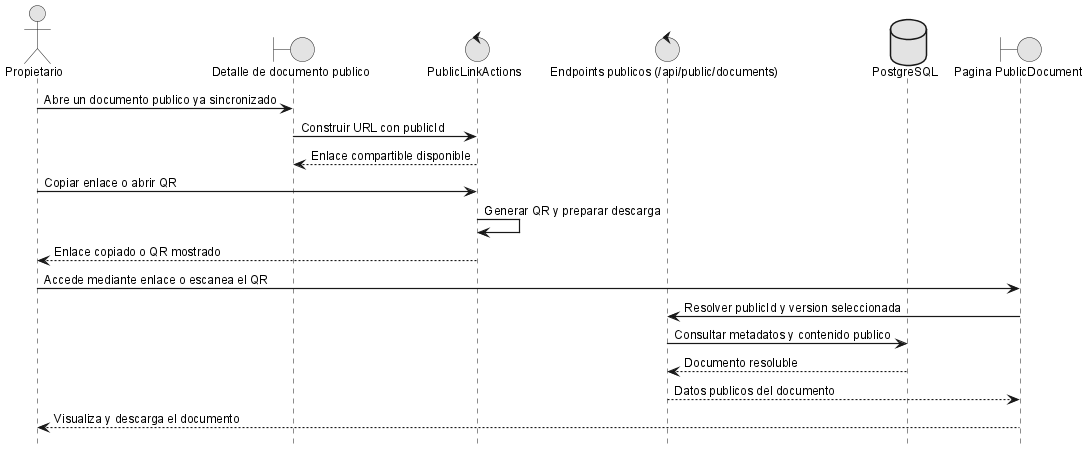
\includegraphics[width=0.92\textwidth]{diagramas/flow-public-link-qr.png}
    \caption{Flujo complementario de distribución por enlace y código QR integrado en UC-0021}
    \label{fig:flow-public-link-qr}
\end{figure}

Este segundo flujo recoge la distribución pública desde la vista de detalle y desde el selector de versiones operativas, donde se generan el enlace resoluble y el código QR asociados al \texttt{publicId} del documento.

\section{Referencia cruzada a los requisitos}

Las siguientes matrices verifican que todos los requisitos del Anexo I tienen cobertura en el diseño de este anexo.

\subsection{Matriz IRQ -- Componente de diseño}

{\setlength{\tabcolsep}{3pt}
\begin{table}[H]
\centering
\footnotesize
\begin{tabular}{|p{2.2cm}|p{3.2cm}|p{4.5cm}|p{4.5cm}|}
\hline
\textbf{Requisito} & \textbf{Entidades clave} & \textbf{Tablas BD} & \textbf{Componentes de diseño} \\
\hline
\hline
IRQ-0001 & Usuario, Wallet, Sesión & users, wallets, sessions & AuthService, WalletService, SessionRepository \\
\hline
IRQ-0002 & Documento, Versión & documents, versions & DocumentService, VersionService, IPFS, Smart Contract \\
\hline
IRQ-0003 & Carpeta, Categoría & folders, categories & FolderService, CategoryService \\
\hline
IRQ-0004 & Firma digital & document\_signatures & SignatureService, Smart Contract \\
\hline
IRQ-0005 & Evento, Auditoría & events & EventService, BlockchainListener \\
\hline
IRQ-0006 & Estadísticas & user\_stats, document\_stats, system\_stats & StatsService \\
\hline
IRQ-0007 & Notificación, Email & notifications, email\_verifications, password\_resets & NotificationService, EmailService \\
\hline
\end{tabular}
\caption{Matriz de trazabilidad IRQ -- componentes de diseño}
\label{tab:cross-irq-design}
\end{table}}

\subsection{Matriz UC -- Clases de análisis}

{\setlength{\tabcolsep}{3pt}
\begin{table}[H]
\centering
\footnotesize
\begin{tabular}{|p{2.7cm}|p{1.4cm}|p{1.4cm}|p{1.4cm}|p{1.6cm}|p{1.4cm}|p{1.4cm}|p{1.4cm}|}
\hline
\textbf{Caso de uso} & \textbf{Usuario} & \textbf{Wallet} & \textbf{Documento} & \textbf{Versión} & \textbf{Carpeta} & \textbf{Firma} & \textbf{Notif.} \\
\hline
\hline
UC-0001 a UC-0018 (Acceso) & X & X & & & & & X \\
\hline
UC-0019 a UC-0028 (Documentos) & X & & X & X & X & & X \\
\hline
UC-0029 a UC-0033 (Versionado) & X & & X & X & & & \\
\hline
UC-0034 a UC-0036 (Firmas) & X & X & X & X & & X & X \\
\hline
UC-0037 a UC-0040 (Compartición) & X & & X & X & X & & X \\
\hline
UC-0041 a UC-0044 (Organización) & X & & X & & X & & \\
\hline
UC-0045 a UC-0048 (Auditoría) & X & & X & X & & & \\
\hline
UC-0049 a UC-0055 (Admin) & X & X & X & & & & X \\
\hline
UC-0056 a UC-0057 (Notificaciones) & X & & & & & & X \\
\hline
\end{tabular}
\caption{Matriz de trazabilidad UC -- clases de análisis}
\label{tab:cross-uc-classes}
\end{table}}

\subsection{Cobertura de requisitos no funcionales}

\begin{table}[H]
\centering
\small
\begin{tabular}{|p{2.5cm}|p{11cm}|}
\hline
\textbf{Requisito} & \textbf{Elementos de diseño que lo satisfacen} \\
\hline
\hline
NFR-0001 (Seguridad) & Cifrado AES-256-GCM en IPFS, Argon2id para passwords, HTTPS forzoso, JWT con rotación, Rate Limiting, validación de entrada en todos los endpoints \\
\hline
NFR-0002 (Rendimiento) & Índices en BD (userId, documentId, eventType), backend IPFS configurable, pool de conexiones Prisma, streaming de archivos grandes \\
\hline
NFR-0003 (Usabilidad) & Interfaz React responsive con Tailwind, feedback inmediato en operaciones async, prototipos validados por flujos de usuario \\
\hline
NFR-0004 (Disponibilidad) & Patrón Prepare/Confirm con reintentos, Circuit Breaker (Pausable), proveedor IPFS configurable con persistencia gestionada o clúster replicado \\
\hline
NFR-0005 (Mantenibilidad) & TypeScript estricto, ESLint, arquitectura en capas con responsabilidades claras, cobertura de tests \\
\hline
NFR-0006 (Portabilidad) & Docker Compose para todos los servicios, variables de entorno para configuración, backend stateless \\
\hline
\end{tabular}
\caption{Cobertura de requisitos no funcionales}
\label{tab:cross-nfr}
\end{table}

\section{Plan de desarrollo e implementación}

\subsection{Diagrama de despliegue}

El diagrama de despliegue muestra la distribución física de los componentes del sistema en los distintos nodos de infraestructura: el servidor backend con sus listeners de eventos, la red Ethereum, una capa de almacenamiento IPFS compatible representada mediante despliegue autoalojado de referencia, la base de datos PostgreSQL y el proveedor de email.

\begin{landscape}
\vspace*{\fill}
\centering
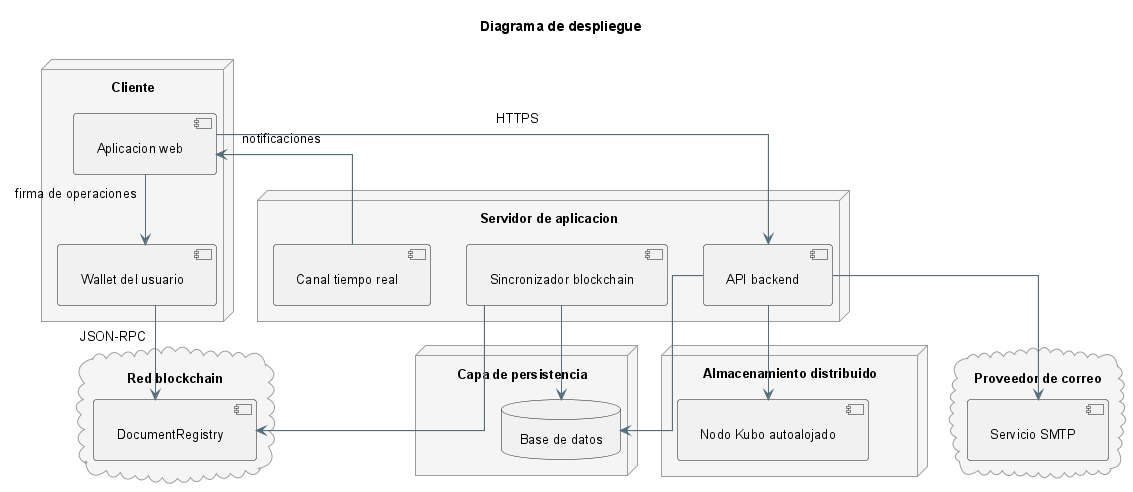
\includegraphics[width=0.95\linewidth]{diagramas/deployment.png}
\captionof{figure}{Diagrama de despliegue completo}
\label{fig:deployment}
\vspace*{\fill}
\end{landscape}

\subsection{Tecnologías de cada componente}

\textbf{Frontend}:
\begin{itemize}
    \item React 18 + TypeScript 5
    \item Vite para build
    \item Tailwind CSS 3
    \item Ethers.js v6 para blockchain
    \item Axios para HTTP
    \item React Router v6
    \item Web Crypto API para descifrado local, hash y gestión de claves en cliente
\end{itemize}

\textbf{Backend}:
\begin{itemize}
    \item Node.js 20 LTS
    \item Express 4
    \item TypeScript 5
    \item Prisma ORM 5
    \item Ethers.js v6
    \item Argon2 para hashing
    \item Nodemailer para emails
    \item WebSocket (ws)
\end{itemize}

\textbf{Base de Datos}:
\begin{itemize}
    \item PostgreSQL 15+
    \item Prisma Migrate para migraciones
\end{itemize}

\textbf{Blockchain}:
\begin{itemize}
    \item Solidity 0.8.20
    \item OpenZeppelin Contracts 5
    \item Hardhat para desarrollo
    \item Ethers.js para interacción
\end{itemize}

\textbf{IPFS}:
\begin{itemize}
    \item IPFS Kubo (go-ipfs)
    \item Pinata Cloud o IPFS Cluster 1.0+
    \item Docker Compose para despliegues autoalojados
\end{itemize}

\section{Glosario}

\textit{(Mismo glosario que Anexo I)}

\section*{Bibliografía}
\addcontentsline{toc}{section}{Bibliografía}

\begin{enumerate}
    \item Gamma, E., Helm, R., Johnson, R., \& Vlissides, J. (1994). \textit{Design Patterns: Elements of Reusable Object-Oriented Software}. Addison-Wesley.
    \item Fowler, M. (2002). \textit{Patterns of Enterprise Application Architecture}. Addison-Wesley.
    \item Evans, E. (2003). \textit{Domain-Driven Design: Tackling Complexity in the Heart of Software}. Addison-Wesley.
    \item OpenZeppelin. (2025). \textit{Smart Contract Patterns}. \url{https://docs.openzeppelin.com/contracts/}
    \item Ethereum Foundation. (2025). \textit{Solidity Documentation}. \url{https://docs.soliditylang.org/}
    \item Protocol Labs. (2025). \textit{IPFS Cluster Documentation}. \url{https://ipfscluster.io/documentation/}
    \item Pinata. (2025). \textit{Pinata Documentation}. \url{https://docs.pinata.cloud/}
    \item React Team. (2025). \textit{React Documentation}. \url{https://react.dev/}
    \item Prisma Team. (2025). \textit{Prisma Documentation}. \url{https://www.prisma.io/docs}
\end{enumerate}

\end{document}
